
% uWaterloo Thesis Template for LaTeX 
% Last Updated May 24, 2011 by Stephen Carr, IST Client Services
% FOR ASSISTANCE, please send mail to rt-IST-CSmathsci@ist.uwaterloo.ca

% Effective October 2006, the University of Waterloo 
% requires electronic thesis submission. See the uWaterloo thesis regulations at
% http://www.grad.uwaterloo.ca/Thesis_Regs/thesistofc.asp.

% DON'T FORGET TO ADD YOUR OWN NAME AND TITLE in the "hyperref" package
% configuration below. THIS INFORMATION GETS EMBEDDED IN THE PDF FINAL PDF DOCUMENT.
% You can view the information if you view Properties of the PDF document.

% Many faculties/departments also require one or more printed
% copies. This template attempts to satisfy both types of output. 
% It is based on the standard "book" document class which provides all necessary 
% sectioning structures and allows multi-part theses.

% DISCLAIMER
% To the best of our knowledge, this template satisfies the current uWaterloo requirements.
% However, it is your responsibility to assure that you have met all 
% requirements of the University and your particular department.
% Many thanks to the feedback from many graduates that assisted the development of this template.

% -----------------------------------------------------------------------

% By default, output is produced that is geared toward generating a PDF 
% version optimized for viewing on an electronic display, including 
% hyperlinks within the PDF.
 
% E.g. to process a thesis called "mythesis.tex" based on this template, run:

% pdflatex mythesis	-- first pass of the pdflatex processor
% bibtex mythesis	-- generates bibliography from .bib data file(s) 
% pdflatex mythesis	-- fixes cross-references, bibliographic references, etc
% pdflatex mythesis	-- fixes cross-references, bibliographic references, etc

% If you use the recommended LaTeX editor, Texmaker, you would open the mythesis.tex
% file, then click the pdflatex button. Then run BibTeX (under the Tools menu).
% Then click the pdflatex button two more times. If you have an index as well,
% you'll need to run MakeIndex from the Tools menu as well, before running pdflatex
% the last two times.

% N.B. The "pdftex" program allows graphics in the following formats to be
% included with the "\includegraphics" command: PNG, PDF, JPEG, TIFF
% Tip 1: Generate your figures and photos in the size you want them to appear
% in your thesis, rather than scaling them with \includegraphics options.
% Tip 2: Any drawings you do should be in scalable vector graphic formats:
% SVG, PNG, WMF, EPS and then converted to PNG or PDF, so they are scalable in
% the final PDF as well.
% Tip 3: Photographs should be cropped and compressed so as not to be too large.

% To create a PDF output that is optimized for double-sided printing: 
%
% 1) comment-out the \documentclass statement in the preamble below, and
% un-comment the second \documentclass line.
%
% 2) change the value assigned below to the boolean variable
% "PrintVersion" from "false" to "true".

% --------------------- Start of Document Preamble -----------------------

% Specify the document class, default style attributes, and page dimensions
% For hyperlinked PDF, suitable for viewing on a computer, use this:
\documentclass[letterpaper,12pt,titlepage,oneside,final]{book}
\usepackage{lineno}
\usepackage{float}
% For PDF, suitable for double-sided printing, change the PrintVersion variable below
% to "true" and use this \documentclass line instead of the one above:
%\documentclass[letterpaper,12pt,titlepage,openright,twoside,final]{book}

% Some LaTeX commands I define for my own nomenclature.
% If you have to, it's better to change nomenclature once here than in a 
% million places throughout your thesis!
\newcommand{\package}[1]{\textbf{#1}} % package names in bold text
\newcommand{\cmmd}[1]{\textbackslash\texttt{#1}} % command name in tt font 
\newcommand{\href}[1]{#1} % does nothing, but defines the command so the
    % print-optimized version will ignore \href tags (redefined by hyperref pkg).
%\newcommand{\texorpdfstring}[2]{#1} % does nothing, but defines the command
% Anything defined here may be redefined by packages added below...

% This package allows if-then-else control structures.
\usepackage{ifthen}
\newboolean{PrintVersion}
\setboolean{PrintVersion}{false} 
% CHANGE THIS VALUE TO "true" as necessary, to improve printed results for hard copies
% by overriding some options of the hyperref package below.

%\usepackage{nomencl} % For a nomenclature (optional; available from ctan.org)
\usepackage{amsmath,amssymb,amstext} % Lots of math symbols and environments
\usepackage{tikz}
%\usepackage[pdftex]{graphicx} % For including graphics N.B. pdftex graphics driver 
%\usepackage{epstopdf}
% Hyperlinks make it very easy to navigate an electronic document.
% In addition, this is where you should specify the thesis title
% and author as they appear in the properties of the PDF document.
% Use the "hyperref" package 
% N.B. HYPERREF MUST BE THE LAST PACKAGE LOADED; ADD ADDITIONAL PKGS ABOVE
\usepackage[pdftex,letterpaper=true,pagebackref=false]{hyperref} % with basic options
		% N.B. pagebackref=true provides links back from the References to the body text. This can cause trouble for printing.
\usepackage{epigraph}
\usepackage{textcomp}
\usepackage{gensymb}
\usepackage{bm}
\hypersetup{
    plainpages=false,       % needed if Roman numbers in frontpages
    pdfpagelabels=true,     % adds page number as label in Acrobat's page count
    bookmarks=true,         % show bookmarks bar?
    unicode=false,          % non-Latin characters in Acrobat’s bookmarks
    pdftoolbar=true,        % show Acrobat’s toolbar?
    pdfmenubar=true,        % show Acrobat’s menu?
    pdffitwindow=false,     % window fit to page when opened
    pdfstartview={FitH},    % fits the width of the page to the window
    pdftitle={Matthew\ Ambacher\ MMath\ Thesis},    % title: CHANGE THIS TEXT!
%    pdfauthor={Author},    % author: CHANGE THIS TEXT! and uncomment this line
%    pdfsubject={Subject},  % subject: CHANGE THIS TEXT! and uncomment this line
%    pdfkeywords={keyword1} {key2} {key3}, % list of keywords, and uncomment this line if desired
    pdfnewwindow=true,      % links in new window
    colorlinks=true,        % false: boxed links; true: colored links
    linkcolor=blue,         % color of internal links
    citecolor=green,        % color of links to bibliography
    filecolor=magenta,      % color of file links
    urlcolor=cyan           % color of external links
}
\ifthenelse{\boolean{PrintVersion}}{   % for improved print quality, change some hyperref options
\hypersetup{	% override some previously defined hyperref options
%    colorlinks,%
    citecolor=black,%
    filecolor=black,%
    linkcolor=black,%
    urlcolor=black}
}{} % end of ifthenelse (no else)

% Setting up the page margins...
% uWaterloo thesis requirements specify a minimum of 1 inch (72pt) margin at the
% top, bottom, and outside page edges and a 1.125 in. (81pt) gutter
% margin (on binding side). While this is not an issue for electronic
% viewing, a PDF may be printed, and so we have the same page layout for
% both printed and electronic versions, we leave the gutter margin in.
% Set margins to minimum permitted by uWaterloo thesis regulations:
\setlength{\marginparwidth}{0pt} % width of margin notes
% N.B. If margin notes are used, you must adjust \textwidth, \marginparwidth
% and \marginparsep so that the space left between the margin notes and page
% edge is less than 15 mm (0.6 in.)
\setlength{\marginparsep}{0pt} % width of space between body text and margin notes
\setlength{\evensidemargin}{0.125in} % Adds 1/8 in. to binding side of all 
% even-numbered pages when the "twoside" printing option is selected
\setlength{\oddsidemargin}{0.125in} % Adds 1/8 in. to the left of all pages
% when "oneside" printing is selected, and to the left of all odd-numbered
% pages when "twoside" printing is selected
\setlength{\textwidth}{6.375in} % assuming US letter paper (8.5 in. x 11 in.) and 
% side margins as above
\raggedbottom

% The following statement specifies the amount of space between
% paragraphs. Other reasonable specifications are \bigskipamount and \smallskipamount.
\setlength{\parskip}{\medskipamount}
\setlength\parindent{0pt}

% The following statement controls the line spacing.  The default
% spacing corresponds to good typographic conventions and only slight
% changes (e.g., perhaps "1.2"), if any, should be made.
\renewcommand{\baselinestretch}{1} % this is the default line space setting

% By default, each chapter will start on a recto (right-hand side)
% page.  We also force each section of the front pages to start on 
% a recto page by inserting \cleardoublepage commands.
% In many cases, this will require that the verso page be
% blank and, while it should be counted, a page number should not be
% printed.  The following statements ensure a page number is not
% printed on an otherwise blank verso page.
\let\origdoublepage\cleardoublepage
\newcommand{\clearemptydoublepage}{%
  \clearpage{\pagestyle{empty}\origdoublepage}}
\let\cleardoublepage\clearemptydoublepage

%======================================================================
%   L O G I C A L    D O C U M E N T -- the content of your thesis
%======================================================================
\begin{document}

% For a large document, it is a good idea to divide your thesis
% into several files, each one containing one chapter.
% To illustrate this idea, the "front pages" (i.e., title page,
% declaration, borrowers' page, abstract, acknowledgements,
% dedication, table of contents, list of tables, list of figures,
% nomenclature) are contained within the file "uw-ethesis-frontpgs.tex" which is
% included into the document by the following statement.
%----------------------------------------------------------------------
% FRONT MATERIAL
%----------------------------------------------------------------------
%\linenumbers
% T I T L E   P A G E
% -------------------
% Last updated May 24, 2011, by Stephen Carr, IST-Client Services
% The title page is counted as page `i' but we need to suppress the
% page number.  We also don't want any headers or footers.
\pagestyle{empty}
\pagenumbering{roman}

% The contents of the title page are specified in the "titlepage"
% environment.
\begin{titlepage}
        \begin{center}
        \vspace*{1.0cm}

        \Huge
        {\bf Normal Mode Wave-Vortex Decompositions of Mesoscale Simulations}

        \vspace*{1.0cm}

        \normalsize
        by \\

        \vspace*{1.0cm}

        \Large
        Matthew R. Ambacher \\

        \vspace*{3.0cm}

        \normalsize
        A thesis \\
        presented to the University of Waterloo \\ 
        in fulfillment of the \\
        thesis requirement for the degree of \\
        Master of Mathematics \\
        in \\
        Applied Mathematics \\

        \vspace*{2.0cm}

        Waterloo, Ontario, Canada, 2017 \\

        \vspace*{1.0cm}

        \copyright\ Matthew R. Ambacher 2017 \\
        \end{center}
\end{titlepage}

% The rest of the front pages should contain no headers and be numbered using Roman numerals starting with `ii'
\pagestyle{plain}
\setcounter{page}{2}

\cleardoublepage % Ends the current page and causes all figures and tables that have so far appeared in the input to be printed.
% In a two-sided printing style, it also makes the next page a right-hand (odd-numbered) page, producing a blank page if necessary.
 


% D E C L A R A T I O N   P A G E
% -------------------------------
  % The following is the sample Delaration Page as provided by the GSO
  % December 13th, 2006.  It is designed for an electronic thesis.
  \noindent
I hereby declare that I am the sole author of this thesis. This is a true copy of the thesis, including any required final revisions, as accepted by my examiners.

  \bigskip
  
  \noindent
I understand that my thesis may be made electronically available to the public.

\cleardoublepage
%\newpage

% A B S T R A C T
% ---------------

\begin{center}\textbf{Abstract}\end{center}

The kinetic energy spectrum of the atmosphere has been well observed to exhibit a $k^{-3}$ power law at synoptic scales with a transition to a shallower $k^{-5/3}$ power law at the mesoscale.  To better understand the mesoscale kinetic energy spectrum, the spectrum can be decomposed into the two dominant modes at this scale: quasi-horizontal vortex motion and inertia-gravity wave motion.  A commonly used technique for this is a Helmholtz decomposition of the horizontal velocity into rotational and divergent components, representing the geostrophically balanced and inertia-gravity wave modes, respectively.  This decomposition is a crude approximation, since geostrophically balanced flows have small but non-zero divergence and inertia-gravity waves can have non-zero rotational energy.\\

We investigate the mesoscale spectrum generated in a moderate-resolution, doubly-periodic, non-hydrostatic simulation of a baroclinically unstable jet.  A three-dimensional normal mode decomposition is used to decompose the total energy into geostrophic and ageostrophic components. We compare the results with the Helmholtz decomposition and find they are qualitatively similar, but ageostrophic modes increasingly dominate with increasing vertical wave number. Specifically, we find the geostrophic mode in the mesoscale to have a steeper spectral slope than the spectral slope of the rotational component of the Helmholtz decomposition at $-3.1$ and $-2.7$, respectively. The difference between the spectral slopes of the ageostrophic and divergent modes are much greater, with mesoscale slope values of $-2.7$ and $-1.9$, respectively. We find that the reason for these differences can be attributed to both the inclusion of the available potential energy in the normal mode decomposition, and the inclusion of rotational energy in the ageostrophic mode of the normal mode decomposition.

\cleardoublepage
%\newpage

% A C K N O W L E D G E M E N T S
% -------------------------------

\begin{center}\textbf{Acknowledgements}\end{center}

First and foremost, I want to thank my supervisor, Mike Waite. Without his help and guidance, this thesis would have never seen the light of day. His availability to meet with me, give feedback, and provide thoughtful discussion (many times of which were on short notice) was integral in finishing this thesis on time. Mike has truly made my two years here an enjoyable time.\\

I would also like to acknowledge my committee members, Francis Poulin and Marek Stastna, for their help over the last two years. Francis' help to better understand the normal mode theory was crucial to setting up simulations and piecing together the results. I want to thank Marek not only for his help and support during my Master's degree, but also going back to my time as an undergrad, where he got me interested in fluid mechanics. \\

Lastly, I want to thank all of the guys in my office: Shawn Corvec, Jonathan Drake, Anthony Caterini, and Tony-Pierre Kim. Thanks for keeping me sane over the past two years.  
\cleardoublepage
%\newpage

% D E D I C A T I O N
% -------------------

\begin{center}\textbf{Dedication}\end{center}

\noindent To my Aunt Maureen, who always encouraged me to pursue the various interests in my life. I wish you were here to read this thesis.

\cleardoublepage
%\newpage

% T A B L E   O F   C O N T E N T S
% ---------------------------------
\renewcommand\contentsname{Table of Contents}
\tableofcontents
\cleardoublepage
\phantomsection
%\newpage

% L I S T   O F   T A B L E S
% ---------------------------
\addcontentsline{toc}{chapter}{List of Tables}
\listoftables
\cleardoublepage
\phantomsection		% allows hyperref to link to the correct page
%\newpage

% L I S T   O F   F I G U R E S
% -----------------------------
\addcontentsline{toc}{chapter}{List of Figures}
\listoffigures
\cleardoublepage
\phantomsection		% allows hyperref to link to the correct page
%\newpage

% L I S T   O F   S Y M B O L S
% -----------------------------
% To include a Nomenclature section
% \addcontentsline{toc}{chapter}{\textbf{Nomenclature}}
% \renewcommand{\nomname}{Nomenclature}
% \printglossary
% \cleardoublepage
% \phantomsection % allows hyperref to link to the correct page
% \newpage

% Change page numbering back to Arabic numerals
\pagenumbering{arabic}
\newpage
 

%----------------------------------------------------------------------
% MAIN BODY
%----------------------------------------------------------------------
% Because this is a short document, and to reduce the number of files
% needed for this template, the chapters are not separate
% documents as suggested above, but you get the idea. If they were
% separate documents, they would each start with the \chapter command, i.e, 
% do not contain \documentclass or \begin{document} and \end{document} commands.
%======================================================================

\newpage
\chapter{Introduction}
\label{ch:ch1}

\section{Background}
\label{sec:introduction}

The atmospheric dynamics on Earth are a complicated process that occur over many length and time scales. At one end, the synoptic scales give rise to large-scale weather events that occur at horizontal length scales on the order of 1000 kilometres, such as hurricanes and tropical storms. The general public is also regularly exposed to the synoptic scale, as high and low-pressure systems seen on weather maps (e.g.\ on local television stations during the morning news) are systems that occur at the synoptic scale. The flow at the synoptic scales is predominantly quasi-geostrophic (QG) in nature, i.e.\ the dominant balance of the momentum equations is between the pressure gradient and Coriolis forces (see Section \ref{sec:geostrophic}). At the other end of the scale spectrum, the microscale encompasses phenomena on horizontal length scales ranging from millimetres up to the order of 1 kilometre, e.g. clouds and small-scale turbulence. As the flow transitions from the synoptic scales to the microscales, the QG approximation becomes less appropriate.\\

Connecting these two scales is the mesoscale, which exists in the range of 10-1000 kilometres \cite{Lin2008}. The mesoscale plays an important role in atmospheric dynamics and weather patterns; it is responsible for storm features, rainfall distribution, fronts, gravity waves, and sea-breeze \cite{Parker2014}. Turbulence in the mesoscale can promote mixing, leading to inhomogeneities in local weather conditions (e.g. surface temperature).\\

The kinetic energy spectrum of the atmosphere was first comprehensively documented by Nastrom and Gage \cite{Nastrom1985} using sensors on commercial aircraft to gather wind velocity and temperature data across many different wavelengths. The authors concluded that the kinetic energy spectrum follows a $k^{-3}$ power law at large scales where the QG approximation is valid, consistent with the QG turbulence theory of Charney \cite{Charney1971}. In the mesoscale, the spectrum shallows to a $k^{-5/3}$ power law, where the QG approximation is increasingly invalid. Since the work done by Nastrom and Gage, researchers have extensively studied this transition numerically \cite{Waite2009,Terasaki2011,Kitamura2010,Hamilton2008,Peng2013,Takahashi2006}.\\

The mesoscale shallowing has been of particular interest to researchers due to open questions about energy transfer through the mesoscale. Initially, it was thought that mesoscale spectrum was due to the inverse cascade of energy from small scales to large scales (e.g.\ \cite{Gage1979, Lilly1983}), analagous to the theory of two-dimensional turbulence first proposed by Kraichnan \cite{Kraichnan1967} . Around the same time, alternative explanations were offered, such as an inertia-gravity wave (IGW) theory proposed by Van Zandt \cite{VanZandt1982}. VanZandt noticed there were similarities to the IGW model of Garrett and Munk \cite{Garrett1972,Garrett1975}, originally used for describing the oceanic spectra. By making slight modifications, VanZandt could fit the atmospheric spectra well. Later on, observations by Lindborg and Cho \cite{Lindborg2001} suggest that the transfer of energy in the mesoscale is a downward cascade of energy from large to small scales, in accordance with isotropic three-dimensional turbulence theory introduced by Kolmogorov in 1941 \cite{Kolmogorov1991}. Over the past decade, the $-3$ power law transition to a shallower spectrum has been reproduced in many numerical simulations, ranging from more idealized simulations of rotating stratified turublence (e.g.\ \cite{Bartello2010,Kitamura2010}) to more complicated simulations employing global models (e.g.\ \cite{Takahashi2006,Hamilton2008}). \\

On average, the atmosphere is stably stratified, which means the two dominant modes of motion are quasi-horizontal vortical motion and IGWs \cite{Riley2000}. Decomposing the flow into these two modes of motion can help understand and link together mesoscale theory and observations. One common technique of separating the flow into vortical and gravity waves is a Helmholtz decomposition of the horizontal velocity fields into rotational and divergent components (e.g.\ \cite{Cho1999,Waite2009,Waite2013}), where the rotational field represents the vortical mode and the divergent field represents the gravity wave mode. Recent work has even been put forth to extract the Helmholtz spectra from one-dimensional data \cite{Callies2016}. Despite the common usage of the Helmholtz decomposition to decompose the flow, it is a very crude decomposition because the balanced vortical component can have small, but non-zero, divergence and IGWs can have non-zero rotational energy. Nevertheless, a Helmholtz decomposition is a simple starting point for examining the kinetic energy spectrum of a rotating, stratified fluid.\\

In this thesis, we employ an improvement to the Helmholtz decomposition by instead considering a normal mode framework derived from the rotating primitive equations to decompose the flow into a geostrophic and ageostrophic components. This decomposition is more realistic; allowing the gravity waves to contain rotational energy as well as divergent energy. As will be seen in Chapter \ref{ch:ch2}, the geostrophic mode is still identically divergence-free. Furthermore, the hydrostatic approximation is used in the development of the normal modes. There are of course many non-hydrostatic features in the atmosphere, but we argue in Chapter \ref{ch:ch3} that our simulation remains fairly hydrostatic. Another advantage to using a normal mode decomposition instead of the Helmholtz decomposition is that the potential energy is included into the geostrophic and ageostrophic modes in addition to the kinetic energy, which may be important to the mesoscale shallowing.\\

Normal mode decompositions of the atmosphere are not a new technique of splitting the flow into geostrophic and ageostrophic components. On one end, very idealized normal mode decompositions such as the triply-periodic, Boussinesq normal mode decomposition by Bartello \cite{Bartello1995} have been used as a starting point for investigating such techniques. On the other end, more realistic normal mode decompositions using spherical coordinates and global data sets (e.g.\ \cite{Terasaki2011}) have had difficulty showing a clear mesoscale transition to a $-5/3$ slope. We aim to study the mesoscale shallowing in between the two extremes, where the normal mode decomposition in this thesis is more realistic than the Bartello 1995 case, but idealized enough that the results can still be interpreted clearly.\\

In the next section, we review the governing equations of a fluid as well as several important approximations, e.g. hydrostasy and geostrophy. We also discuss the shallow water approximation and Helmholtz decomposition as they will be seen in Chapters \ref{ch:ch2} and \ref{ch:ch4} respectively. Chapter \ref{ch:ch2} derives the normal mode theory used in this simulation. First, it is shown that the vertical structure is determined by a Sturm-Liouville eigenvalue problem for the ageostrophic modes. For the geostrophic mode, there is no explicit vertical structure, and so we propose using the same vertical modes as the ageostrophic mode. It is then shown that each vertical mode corresponds to a shallow water system with an equivalent depth arising from the eigenvalue associated with the vertical eigenfunction. Chapter \ref{ch:ch3} describes the numerical model and setup of the baroclinic instability simulation. Model choice and initialization techniques are described. An overview of the simulation, including horizontal vorticity and velocity snapshots throughout the baroclinic life cycle are shown. Chapter \ref{ch:ch4} presents results of the normal mode decomposition applied to the simulation described in Chapter \ref{ch:ch3}. Comparisons to the Helmholtz decomposition are made. Due to the large number of vertical modes examined, most of the discussion is delayed until Chapter \ref{ch:ch5}. In Chapter \ref{ch:ch5}, we discuss the results obtained in Chapter \ref{ch:ch4}. Differences between the Helmholtz and normal mode decompositions are examined and we present key differences in the mesoscale spectra. Lastly, we offer concluding marks on the normal mode decomposition.

\section{Mathematical Preliminaries}
\label{sec:preliminaries}
The governing equations of motion of a viscous, heat conducting fluid are a set of partial differential equations called the Navier-Stokes equations. In this section, the governing equations are described, as well as simplifications to these equations and assumptions used in the remainder of this thesis. In addition, single-layer shallow water theory is discussed, as well as the Helmholtz decomposition. In this section, we use $\mathbf{v} = (u,v,w)$ to represent the full three-dimensional velocity field and $\mathbf{u} = (u,v)$ to be the horizontal velocity field. When pressure coordinates are introduced in Section \ref{sec:pressurecoords}, we keep the horizontal and vertical components separate for clarity. Operators acting on $\mathbf{u}$ and $\mathbf{v}$ are understood to be two- or three-dimensional, respectively. For example $\nabla \cdot \mathbf{u} = \partial u/\partial x + \partial v/\partial y$, while $\nabla \cdot \mathbf{v} = \partial u/\partial x + \partial v/\partial y + \partial w/\partial z$. The mathematical background presented in this section can be found in any fluid mechanics text. We have followed Kundu and Cohen \cite{Kundu2002} for Sections \ref{sec:momentum}, \ref{sec:coriolis}, \ref{sec:hydrostatic}, and \ref{sec:geostrophic}. For Sections \ref{sec:eos}, \ref{sec:pressurecoords}, \ref{sec:APE}, and \ref{sec:shallowwater} we have followed Vallis \cite{Vallis2006}.

\subsection{Mass Continuity and Momentum Equations}
\label{sec:momentum}
The conservation of mass is one of the fundamental conservation laws in classical mechanics. The conservation of mass for a fluid can be understood by considering a small control volume fixed in space. The conservation of mass must take into account the amount of fluid entering and exiting the control volume, as well as the density of fluid inside this control volume as it may change with time. The conservation of mass can thus be written as
\begin{align}
\frac{\partial \rho}{\partial t} + \nabla \cdot (\rho \mathbf{v}) = 0 \label{eq:continuityGeneral},
\end{align} 
with $\mathbf{v} = (u,v,w)$ representing the full three dimensional wind. In addition to equation (\ref{eq:continuityGeneral}), there are also momentum equations. The momentum equations describe how a fluid's motion is influenced by external forces acting on the fluid. The momentum equations are written in vector form as follows

\begin{align}
\frac{\partial \mathbf{v}}{\partial t} + (\mathbf{v} \cdot \nabla)\mathbf{v}  = -\frac{1}{\rho} \nabla p + \nu \nabla^2 \mathbf{v} + \mathbf{F_b}. \label{eq:momentumGeneral}
\end{align}

Each term in the momentum equations have physical interpretations that make their contributions clear:
\begin{itemize}
\item[] $\partial \mathbf{v}/\partial t$ represents the local acceleration of the fluid at a fixed location in space,

\item[] $(\mathbf{v} \cdot \nabla) \mathbf{v}$ is the advection of velocity of a fluid parcel by the surrounding flow,

\item[] $\nabla p$ is the pressure gradient term with the negative sign indicating flow moves from high to low pressure,

\item[] $\nu \nabla^2 \mathbf{v}$ is the viscous dissipation, where $\nu$ is a property of the fluid. For air, $\nu$ is approximately $1.5 \times 10^{-5}~ \text{m}^2~\text{s}^{-1}$,

\item[] $\mathbf{F_b}$ contains the body forces (e.g. gravity).
\end{itemize}

A simplification to the full Navier-Stokes equations are the Euler equations, which consider inviscid, adiabatic flow. In this thesis, we use the Euler equations and drop the viscosity term. In the simulation described in Chapter \ref{ch:ch3}, however, we will include weak numerical viscosity to dissipate energy. Equation (\ref{eq:momentumGeneral}) can then be written
\begin{align}
\frac{\text{D}\mathbf{v}}{\text{D}t}  = -\frac{1}{\rho} \nabla p + \mathbf{F_b} \label{eq:momentumEuler},
\end{align}

where the notation $\text{D}/\text{D}t = \partial/\partial t + \mathbf{v} \cdot \nabla$ is called the material derivative operator.\\

Note that both the continuity (\ref{eq:continuityGeneral}) and momentum equations (\ref{eq:momentumGeneral}) are written in a coordinate-free manner. Section \ref{sec:pressurecoords} considers a pressure-based vertical coordinate. Also of note is that equations (\ref{eq:momentumGeneral}) do not consider the effects of rotation. Section \ref{sec:coriolis} discusses the momentum equations in a non-inertial reference frame.

\subsection{Equation of State and a Thermodynamic Equation}
\label{sec:eos}
The mass continuity equation (\ref{eq:continuityGeneral}) and momentum equations (\ref{eq:momentumGeneral}) give a system of equations with 5 unknowns with only 4 equations. To close the system, we require an equation of state. An equation of state is a function relating the pressure field of a flow to the density $\rho$, temperature $T$, and composition $S$. We write the general form of the equation of state as
\begin{align}
p = f(\rho, T, S). \label{eq:eosGeneral}
\end{align}

In this thesis, only Earth's atmosphere (air) is considered which can be well approximated as having constant composition, when water vapor is not included. The pressure can be related to the density and temperature by the ideal gas law . The explicit form of the the equation of state for air can thus be written as 
\begin{align}
p = \rho RT = \rho R \theta \left( \frac{p}{p_s} \right) ^ {-R/c_{p}}, \label{eq:eos}\\
\theta = T \left( \frac{p}{p_s} \right)^{-R/c_p}, \label{eq:potTemp}
\end{align}
where $R$ is the ideal gas constant ($287 ~\text{J}~\text{kg}^{-1}~\text{K}^{-1}$), $p_s$ is the surface pressure ($10^5 ~\text{Pa}$), $c_p$ is the heat capacity at constant pressure ($1004.5 ~\text{J}~\text{kg}^{-1}~\text{K}^{-1}$ for air). $\theta$ is the potential temperature, which is the temperature that a fluid parcel would have if moved adiabatically to a reference pressure, which we take to be 1000 mbar. Potential temperature is a conserved quantity if the flow is adiabatic, as seen in equation (\ref{eq:thermoGeneral}).\\

By introducing the equation of state (\ref{eq:eos}), the relationship between pressure and density provided the fifth equation for the five unknowns. However, the equation of state (\ref{eq:eos}) also introduced another unknown, namely the potential temperature. We thus require a thermodynamic equation to close the system. The general form of the thermodynamic equation can be written as 
\begin{align}
\frac{\text{D}\theta}{\text{D}t} = Q, \label{eq:thermoGeneral}
\end{align}
where $Q$ is the change in potential temperature due to all diabatic sources and sinks. As this thesis considers an adiabatic ideal gas, i.e. we can rewrite equation (\ref{eq:thermoGeneral}) as 
\begin{align}
\frac{\text{D}\theta}{\text{D}t} = 0.\label{eq:thermo}
\end{align}

\subsection{Rotating Frame of Reference}
\label{sec:coriolis}
The momentum equations (\ref{eq:momentumEuler}) do not consider the effects of a non-inertial reference frame (e.g. the rotating Earth). The rotation of the earth introduces a pseudo force called the Coriolis force which adds a term to the momentum equations. We can rewrite the momentum equations (\ref{eq:momentumEuler}) as
\begin{align}
\frac{\partial \mathbf{v}}{\partial t} + (\mathbf{v} \cdot \nabla)\mathbf{v} + f \mathbf{\hat{k}} \times \mathbf{v}                                                                                                                                                                                                                                                                                                                                                                                                                                                                                                                                                                                                                                                                                                                                                                                                                                                                                                                                                                                                                                                                                                                                                                                                                                                                                                                                                                                                                                                            = -\frac{1}{\rho} \nabla p  + \mathbf{F_b}, \label{eq:momentum}
\end{align}
where $f$ is the Coriolis parameter.\\

This thesis will focus on a mid-latitude baroclinic jet on an $f$-plane. Therefore, we will approximate the Coriolis parameter as $f \approx f_0 = 2\Omega \sin{45^\circ}$, where $\Omega$ is the angular rotation rate of the Earth.

\subsection{Hydrostatic Balance}
\label{sec:hydrostatic}
The vertical component of the momentum equation (\ref{eq:momentum}) can be written explicitly as
\begin{align}
\frac{\text{D} w}{\text{D} t} = -\frac{1}{\rho} \frac{\partial p}{\partial z} - g,
\end{align} 
where $g$ is the acceleration due to gravity. Hydrostatic balance is the assumption that vertical acceleration of a fluid is small and the dominant balance of the vertical momentum equation lies between the pressure gradient and the buoyant forces. This results in the hydrostatic equation 
\begin{align}
\frac{\partial p}{\partial z} = -\rho g \label{eq:hydrostaticZ}.
\end{align}

When the aspect ratio of the flow is small, i.e.\ $H/L \ll 1$, the hydrostatic approximation becomes very good for a flow. The effects of stratification on hydrostasy are also important, under which the condition for hydrostatic balance becomes $\mathrm{Fr}^2(H/L)^2 \ll 1$, where Fr is the Froude number, $Fr = U/NH$ \cite{Vallis2006}. The Froude number is a measure of the stratification of a fluid, and is discussed more in Section \ref{sec:simulationOverview}. In the atmosphere, the troposphere has a depth of around $10$ km, so flows with much larger horizontal scales are approximately in hydrostatic balance.

\subsection{Pressure Coordinates}
\label{sec:pressurecoords}
From the hydrostatic equation (\ref{eq:hydrostaticZ}), since pressure is monotonically decreasing with increasing height it is possible to use this hydrostatic pressure as a vertical coordinate instead of $z$. Indeed, it is advantageous, when working with the hydrostatic equations, to use a vertical coordinate based on hydrostatic pressure instead of geometric height ($z$) when considering geophysical applications in the atmosphere for several reasons. The most prominent reason is that the explicit dependence on density drops out of the pressure gradient term. Consider the horizontal pressure gradient term of equation (\ref{eq:momentumGeneral}) in the $x$-direction,

\begin{align}
-\frac{1}{\rho} \frac{\partial p}{\partial x} = -\frac{1}{\rho} \left(\frac{\partial p}{\partial z}\right)_x \left(\frac{\partial z}{\partial x}\right)_p,
\end{align}
where subscripts on derivatives on the right-hand side indicate quantities being held constant in the evaluation of the derivative. Using hydrostatic balance gives
\begin{align}
-\frac{1}{\rho} \frac{\partial p}{\partial x} &=  g \left(\frac{\partial z}{\partial x}\right)_p,\\
&= \left( \frac{\partial \Phi}{\partial x}\right)_p,
\end{align}
and similarly for the pressure gradient in the $y-$ direction. $\Phi = gz$ is the geopotential height, which is evaluated along constant pressure levels for the horizontal momentum equations.\\

The continuity equation (\ref{eq:continuityGeneral}) also simplifies under hydrostatic pressure coordinates to yield

\begin{align}
\frac{\partial u}{\partial x} + \frac{\partial v}{\partial y} + \frac{\partial \omega}{\partial p} = 0,\label{eq:continuity}
\end{align}
where $\omega = \text{D}p/\text{D}t$ is the vertical velocity in pressure coordinates.\\

Finally, by using hydrostatic pressure as the vertical coordinate, hydrostatic balance can be written as
\begin{align}
\frac{\partial \Phi}{\partial p} = -\frac{RT}{P}. \label{eq:hydrostatic}
\end{align}

As a result, the thermodynamic equation can be written in terms of $\Phi$ (see equation (\ref{eq:thermodynamic}) below).

\subsection{Geostrophic Balance} 
\label{sec:geostrophic}
Now consider the horizontal momentum equations (\ref{eq:continuity}). Let $U$ and $L$ be the characteristic horizontal velocity and length scales such that $\mathbf{u} = U \mathbf{\hat{u}}$ and $(x,y) = L(\hat{x},\hat{y})$. Furthermore, assume that time scales advectively (i.e.\ $t = T \hat{t} = L/U \hat{t}$) and non-dimensionalize the equations as follows:

\begin{align}
\frac{U^2}{L} \frac{\partial \mathbf{\hat{u}}}{\partial \hat{t}} + \frac{U^2}{L} (\mathbf{\hat{u}} \cdot \nabla) \mathbf{\hat{u}} + fU (\mathbf{\hat{f}} \times \mathbf{\hat{u}}) = -\nabla \Phi.
\end{align}

The ratio of the advective and Coriolis terms is called the Rossby number \cite{Vallis2006} 
\begin{align}
Ro \equiv \frac{U}{fL},
\end{align}
and is a measure of how important the Coriolis acceleration is. As $Ro \to 0$, the dominant balance in the horizontal momentum equations is between the Coriolis and geopotential terms 
\begin{align}
\mathbf{f}\times\mathbf{u} = -\nabla \Phi.
\end{align}
Note the geostrophic wind is completely determined by horizontal gradients of the geopotential since hyrostatic pressure was used as the vertical coordinate. It is even possible to use hydrostatic pressure as a vertical coordinate when working in a non-hydrostatic environment (see Section \ref{sec:simulationOverview}).

\subsection{Vertical Stratification}
The static stability, $\Gamma$, is a measure of the the vertical stratification of the atmosphere; if the atmosphere is stable, then $\Gamma > 0$. The static stability, in hydrostatic pressure coordinates, is given by
\begin{align}
\Gamma = \frac{1}{p} \frac{\partial}{\partial p}\left( \frac{\partial \Phi}{\partial p} - \frac{R \Phi}{c_p}\right) \label{eq:staticstability},
\end{align}
where $c_p$ is the specific heat capacity of air at constant pressure. The static stability can be rewritten to show the relation to another measure of the vertical stability, the Brunt-V\"ais\"al\"a frequency, $N$, by 
\begin{align}
\Gamma = \frac{N^2}{g^2} \left( \frac{\partial \Phi}{\partial p}\right)^2,
\end{align}
where $N^2 = \dfrac{g}{\theta} \dfrac{\partial \theta}{\partial z}$. When a fluid parcel is displaced in a stably stratified atmosphere, it will oscillate at the Brunt-V\"ais\"al\"a frequency around its equilibrium state.  Using the hydrostatic equation (\ref{eq:hydrostatic}) together with the static stability (\ref{eq:staticstability}), the thermodynamic equation (\ref{eq:thermo}) is

\begin{align}
\left(\frac{\partial}{\partial t} + \mathbf{u} \cdot \nabla\right) \frac{\partial \Phi}{\partial p} + \omega \Gamma = 0. \label{eq:thermodynamic}
\end{align}

\subsection{Summary of Governing Equations}
In this thesis, we make use of the hydrostatic approximation and treat the atmosphere as inviscid to formulate the normal mode decomposition outlined in Chapter \ref{ch:ch2}. The governing equations in pressure coordinates are thus:
\begin{align}
\frac{\partial \mathbf{u}}{\partial t} + (\mathbf{u} \cdot \nabla) \mathbf{u} + \omega \frac{\partial \mathbf{u}}{\partial p} + f \mathbf{k} \times \mathbf{u}& = -\nabla \Phi, \label{eq:momentumFull}\\
\frac{\partial \Phi}{\partial p} &= -\frac{RT}{p},\label{eq:hydrostaticFull}\\
\nabla \cdot \mathbf{u} + \frac{\partial \omega}{\partial p} &= 0,\label{eq:continuityFull}\\
\left(\frac{\partial}{\partial t} + \mathbf{u} \cdot \nabla\right) \frac{\partial \Phi}{\partial p} + \omega \Gamma &= 0. \label{eq:thermodynamicFull}
\end{align}

\subsection{Shallow Water Equations}
\label{sec:shallowwater}
When the horizontal scale of a flow is large compared to the depth, and the density in the fluid is constant, the flow dynamics follow shallow water theory \cite{Vallis2006}. In Chapter \ref{ch:ch2}, we will see that the normal mode decomposition results in a shallow water system associated with each vertical mode. Figure \ref{fig:shallowwater} shows an example of a single-layer shallow water system.\\

\begin{figure}[H]
\begin{center}
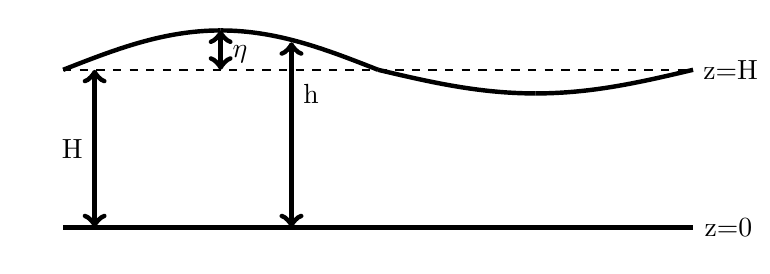
\begin{tikzpicture}
\draw[black,ultra thick] (-4,0) -- (4,0) node[anchor=west]{z=0};
\draw[black, dashed, thick] (-4,2) -- (4,2) node[anchor=west]{z=H};
\draw[black, ultra thick] (-4,2) sin (-2, 2.5);
\draw[black, ultra thick] (-2,2.5) cos (0, 2);
\draw[black, ultra thick] (0,2) sin (2, 1.7);
\draw[black, ultra thick] (2,1.7) cos (4, 2);
\draw[<-, black, line width=2pt] (-3.6,0) -- (-3.6,1) node[anchor=east] {H};
\draw[->, black, line width=2pt] (-3.6,1) -- (-3.6,2);
\draw[<-, black, line width=2pt] (-2,2) -- (-2,2.2) node[anchor=west] {$\eta$};
\draw[->, black, line width=2pt] (-2,2.2) -- (-2,2.5);
\draw[<-, black, line width=2pt] (-1.1,0) -- (-1.1,1.7) node[anchor=west] {h};
\draw[->, black, line width=2pt] (-1.1,1.7) -- (-1.1,2.35);
\end{tikzpicture}
\caption{Single layer shallow water system. H is the mean depth of the fluid, $\eta$ is the fluctuation from the mean, and $\mathrm{h} = \mathrm{H} + \eta$ is the total height of the fluid column.}
\label{fig:shallowwater}
\end{center}
\end{figure}
Shallow water theory uses hydrostatic balance for the vertical momentum equation. Since the density is assumed constant, the hydrostatic equation (\ref{eq:hydrostaticZ}) can be trivially integrated to express the pressure at a height $z$
\begin{align}
p(x,y,z,t) = -\rho g (z - \eta(x,y,t)).
\end{align}

The pressure gradient in the horizontal momentum equations is then simply
\begin{align}
\nabla_H p = \rho g \nabla_H \eta,
\end{align}
with $\nabla_H = (\partial/\partial x, \partial/\partial y)$. Thus the horizontal momentum equations in a single-layer shallow water system are 
\begin{align}
\frac{\partial \mathbf{u}}{\partial t} + (\mathbf{u} \cdot \nabla_H) \mathbf{u} + f \mathbf{k} \times \mathbf{u} = -g \nabla_H \eta.
\end{align}

Mass conservation can be derived by considering the mass flux into a cylindrical column of height $h$ and cross-sectional area $A$. Following Vallis \cite{Vallis2006},

\begin{align}
\text{Mass flux in} &= -\int_s \rho \mathbf{u} \cdot \text{d}S,
\end{align}
where $S$ is the area of the vertical boundary of the water column. If there is a net flux into the column, the height of the column must increase. Writing the surface area as $S = h\mathbf{n}\text{d}l$, where $\text{d}l$ is a line element of the closed curve $\mathcal{C}$ that encompasses the column and $\mathbf{n}$ is the outward pointing normal, then
\begin{align}
&= -\oint_{\mathcal{C}} \rho h\mathbf{u} \cdot \mathbf{n} ~\text{d}l,\\
&= -\int_A  \nabla \cdot (\rho\mathbf{u}h) ~\text{d}A.
\end{align}
The full mass conservation is then
\begin{align} 
&\frac{\text{d}}{\text{d}t} ~\int_V \rho \text{d}V = -\int_A  \nabla \cdot (\rho\mathbf{u}h) ~\text{d}A,\\
&\frac{\text{d}}{\text{d}t} ~\int_A \rho h \text{d}A = -\int_A  \nabla \cdot (\rho\mathbf{u}h)~ \text{d}A,\\
&\int_A \left[\rho \frac{\partial h}{\partial t} + \nabla \cdot (\rho\mathbf{u}h) \right]\text{d}A = 0.
\end{align}
Since the area integrated over is arbitrary, the integrand vanishes, leaving
\begin{align}
\frac{\partial h}{\partial t} + \nabla \cdot (\mathbf{u}h) = 0.
\end{align}

\subsection{Available Potential Energy}
\label{sec:APE}

In general, a conversion between kinetic, internal, and potential energy occurs in a flow. In the case of adiabatic, inviscid flow, the total energy is also conserved. In a stratified flow, not all of the potential energy can be converted to kinetic energy. Some of this potential energy is locked into the background state and is not free for extraction. The available potential energy, as the name suggests, is the amount of potential energy that is available for conversion. It is formally defined by Vallis as the difference between the potential energy of the initial state and the potential energy after an adiabatic arrangement to where the isentropic surfaces are flat.\\

\subsection{Helmholtz Decomposition}
\label{sec:helmholtz}
The domain-averaged kinetic energy can be written as 
\begin{align}
\text{E}_{k} = \frac{1}{2 V} \iiint \rho\left( \mathbf{u}\cdot \mathbf{u} + w^2\right) \text{d}V.
\end{align}
where $V$ is the volume of the domain. Since this is a cubic quantity in the unknowns, the energy is a sum over triads of wavevectors. To simplify this, since density perturbations from the base-state are small, we can instead consider only the base-state of the density, $\overline{\rho}$. The $w^2$ term can also be ignored because it is small compared to the horizontal velocities. The domain-averaged kinetic energy can now be written as
\begin{align}
\text{E}_{k} = \frac{1}{2V} \iiint \overline{\rho} \left(\mathbf{u}\cdot\mathbf{u}\right) \text{d}V. \label{eq:KE}
\end{align}

To study the kinetic energy contained at the different scales, it is useful to write the kinetic energy as a function of wavevectors. One way to do this, assuming horizontally periodic boundary conditions, is to use a two-dimensional discrete Fourier transform on the horizontal velocity fields at each vertical level, which yields a set of spectral coefficients. Through Parseval's theorem, the kinetic energy in the domain can be related to these spectra coefficients. That is, denoting $\widehat{q}(\mathbf{k})$ as the Fourier spectral coefficients of the field $q$, we have Parseval's theorem for a discrete Fourier transform

\begin{align}
 \frac{1}{N_x N_y} \sum_{m=0}^{N_x-1} \sum_{n=0}^{N_y-1} |q_{m,n}|^2 = \sum_{i=0}^{N_x-1}  \sum_{j=0}^{N_y-1} |\widehat{q}_{i,j}|^2.
\end{align}

With the kinetic energy is expressed as a function of the wavenumbers, a natural extension is to decompose the energy into its two dominant modes of motion: vortical and inertia gravity wave (IGW) motion. As outlined in Section \ref{sec:introduction}, one way to decompose the kinetic energy (equation \ref{eq:KE}) into slow vortical and fast wave motion is to apply a Helmholtz decomposition to the velocity fields. Helmholtz's theorem (for review, refer to \cite{Griffiths2013}) states that for a twice-differentiable bounded vector field $\mathbf{F}$ in $\mathbb{R}^2$, one can write the vector field as a combination of a rotational component $\mathbf{k} \times \nabla \mathbf{\psi}$, and an irrotational component $\Phi$,

\begin{align}
\mathbf{F} = \nabla \Phi + \mathbf{k}\times \nabla \mathbf{\psi}, \label{eq:helmholtz}
\end{align}

where $\psi$ is the streamfunction defined by $u = -\partial \psi/\partial y, v = \partial \psi/\partial x$. The resulting rotational field can be used as an analogue to the vortical motion, while the irrotational part can represent the inertia-gravity wave motion. To first compute the horizontal kinetic energy spectrum, which shows the kinetic energy as a function of the wavelength, we use a two-dimensional discrete Fourier transform. By Parseval's theorem, the kinetic energy in the domain can be related to the spectral coefficients given by the Fourier transform. Then using the Helmholtz decomposition, the kinetic energy spectrum can be written in terms of a rotational spectrum and a divergent spectrum.\\

 The divergent kinetic energy (DKE) for a specific horizontal wavevector is given by

\begin{align}
\text{E}_D(\mathbf{k}) = \frac{1}{2} \overline{\rho} \frac{ \bm{\widehat{\delta}}_{k,l} \cdot \bm{\widehat{\delta}}_{k,l}^*}{|\mathbf{k}|}, \label{eq:DKE}
\end{align}

where $\widehat{\delta}_{k,l} = ik\widehat{u}(\mathbf{k}) + il\widehat{v}(\mathbf{k})$ is the horizontal divergence, * denotes the complex conjugate, and $|\mathbf{k}| = \sqrt{k^2 + l^2}$ is the magnitude of the horizontal wavevector  $\mathbf{k} = (k,l)$. In similar fashion, the rotational kinetic energy (RKE) is written

\begin{align}
\text{E}_R (\mathbf{k})= \frac{1}{2} \overline{\rho} \frac{\bm{\widehat{\zeta}}_{k,l} \cdot \bm{\widehat{\zeta}}_{k,l}^*}{|\mathbf{k}|}, \label{eq:RKE}
\end{align}

with $\widehat{\zeta}_{k,l} = ik\widehat{v}(\mathbf{k}) - il\widehat{u}(\mathbf{k})$ as the vertical component of vorticity. When combined, equations (\ref{eq:DKE}) and (\ref{eq:RKE}) give

\begin{align}
\text{E}_R(\mathbf{k}) + \text{E}_D(\mathbf{k}) = \frac{1}{2} \overline{\rho} \left( |\widehat{u}(\mathbf{k})|^2 + |\widehat{v}(\mathbf{k})|^2 \right),
\end{align}

which is the total (rotational plus divergent) kinetic energy at a specific wavevector. 
\newpage
\chapter{Mode Decomposition}
\label{ch:ch2}

\section{Vertical and Horizontal Structure Equations}
The main goal of decomposing the energy spectra into geostrophic and ageostrophic motion is to separate the fast gravity waves from the slow balanced vortices. To that end, consider linearizing the governing equations (\ref{eq:momentumFull} -\ref{eq:thermodynamicFull}) about a state of rest, as commonly done in the literature (e.g.\ \cite{Daley1991}, \cite{Kasahara1981}). While a more complicated basic state can be used (e.g.\ a non-zero zonal mean flow), the primary interest is of the inertia gravity wave modes that are initialized by the baroclinic instabilities. These gravity wave modes have  much shorter characteristic timescales than the slowly rotating geostrophic part and are not strongly influenced by a linearization about a more realistic basic state involving the zonal mean velocity field, e.g.\ \cite{Dickinson1972}. The equations of motion linearized about a state of rest with a basic state geopotential $\tilde{\Phi}$ then result in the following system of equations

\begin{align}
&\frac{\partial u'} {\partial t} - fv' = -\frac{\partial \Phi'}{\partial x},\label{eq:nmMomentum}\\
&\frac{\partial v'} {\partial t} + fu' = -\frac{\partial \Phi'}{\partial y},\\
&\nabla \cdot \mathbf{u'} + \frac{\partial \omega}{\partial p} = 0,\label{eq:nmCont}\\
&\frac{\partial}{\partial t} \frac{\partial \tilde{\Phi}}{\partial p} + \omega \tilde{\Gamma} \label{eq:nmThermo} = 0.
\end{align}

For the rest of this section, the prime notation seen on $u$, $v$, and $\Phi$ to represent the deviation from the basic state is omitted except for where confusion would occur otherwise. Following the approach of Daley \cite{Daley1991}, equations (\ref{eq:nmCont}) and (\ref{eq:nmThermo}) can be combined to reduce the system of equations to three equations and three unknowns shown below:

\begin{align}
&\frac{\partial u} {\partial t} - fv = -\frac{\partial \Phi}{\partial x},\label{eq:nmLinMom}\\
&\frac{\partial v} {\partial t} + fu = -\frac{\partial \Phi}{\partial y},\\
&\frac{\partial}{\partial p} \left( \frac{1}{\tilde{\Gamma}} \frac{\partial }{\partial t} \frac{\partial \tilde{\Phi}}{\partial p}\right) - \nabla \cdot \mathbf{u} = 0. \label{eq:nmThermoHydro}
\end{align}

Since (\ref{eq:nmThermoHydro}) contains all of the explicit vertical derivatives, it is appropriate to separate the vertical dependence of the velocity and geopotential fields from the horizontal dependence, i.e.\ let 
\begin{align}
&u(x,y,p,t) = U(x,y,t) Z(p),\label{eq:separationBegin}\\
&v(x,y,p,t) = V(x,y,t) Z(p),\\
&\Phi(x,y,p,t) = \Phi^*(x,y,t) Z(p).\label{eq:separationEnd}
\end{align}
Substituting this separation into equations (\ref{eq:nmLinMom} - \ref{eq:nmThermoHydro}) gives
\begin{align}
&\frac{\partial U}{\partial t} - fV = -\frac{\partial \Phi^*}{\partial x},\\
&\frac{\partial V}{\partial t} + fU = -\frac{\partial \Phi^*}{\partial y},\\
&\frac{1}{Z}\frac{\text{d}}{\text{d} p} \left(\frac{1}{\tilde{\Gamma}}\frac{\text{d} Z}{\text{d} p}\right) = \frac{1}{\frac{\partial \Phi^*}{\partial t}} \left(\frac{\partial U}{\partial x} + \frac{\partial V}{\partial y}\right) = -\frac{1}{gh_n}, \label{eq:separation}
\end{align}
where $-1/gh$ is a separation constant chosen to be dimensionally consistent with the left-hand side and middle of equation (\ref{eq:separation}). The equations of motion are now in a separated state consisting of horizontal structure

\begin{align}
&\frac{\partial U}{\partial t} - fV = -\frac{\partial \Phi^*}{\partial x}, \label{eq:nmHorizBegin}\\
&\frac{\partial V}{\partial t} + fU = -\frac{\partial \Phi^*}{\partial y},\\
&\left(\frac{\partial U}{\partial x} + \frac{\partial V}{\partial y}\right) + \frac{1}{gh_n} \frac{\partial \Phi^*}{\partial t} = 0, \label{eq:nmHorizEnd}
\end{align}
and vertical structure
\begin{align}
\frac{\text{d}}{\text{d} p} \left( \frac{1}{\tilde{\Gamma}}\frac{\text{d} Z}{\text{d} p} \right) + \frac{1}{gh_n} Z = 0, \label{eq:nmVert}
\end{align}
coupled together by the $1/gh_n$ term. This coupling is only valid if the divergence is non-zero. Note that the horizontal eigenvalue problem is valid only for an $f$-plane approximation and that a $\beta$-plane approximation would result in a different eigenvalue problem in the horizontal. Later in this chapter, the case of geostrophic motion is dealt with. Bearing this in mind, we now focus our attention solely on the vertical structure problem (\ref{eq:nmVert}) of a flow with non-zero divergence, returning to the horizontal problem in Section \ref{sec:horiz} and geostrophic motion in Section \ref{sec:geostrophicMotion} .

\section{Vertical Normal Modes}
\subsection{A Brief Outline of Sturm-Liouville Theory}
A Sturm-Liouville (S-L) problem is a type of ordinary differential equation (ODE) of the form
\begin{align}
\frac{\text{d}}{\text{d} p} \left( s(p) \frac{\text{d} Z}{\text{d} p} \right) + q(p) Z + \lambda w(p) Z = 0, \label{eq:SturmLiouville}
\end{align}
with non-zero $s(p)$ and $w(p)$. Here, $s(p)$, $q(p)$, and $w(p)$ are given functions, with $w(p)$ being the ``weighting'' function. This is an eigenvalue problem, with eigenvalue $\lambda$. There are many nice properties of solutions of S-L problems. We are interested in the orthogonality of eigenfunctions with respect to the weighting $w(p)$ and the guarantee of real, non-degenerate eigenvalues. That is, the eigenvalues can be arranged in an increasing order, and the inner product with respect to $w$ gives an orthonormality condition 
\begin{align}
(f_j, f_k)_w = \int_a^b \overline{f_j(p)}f_k(p) w(p) ~\text{d}p = \delta_{jk} \label{eq:orthonormamiltyHard}
\end{align}
for normalized eigenfunctions $f_j(p)$, $f_k(p)$ and appropriate boundary conditions at $p=a,b$. In addition to the orthogonality, eigenfunctions of a S-L problem are complete. Refer to any ODE text for a review (e.g. \cite{Atkinson1964}).\\

From this, it is clear that the vertical structure equation (\ref{eq:nmVert}) is a S-L ODE with $q(p) = 0$ and $s(p) = 1/\tilde{\Gamma}(p)$, $\lambda = 1/gh$, and $w(p) = 1$. The orthogonality condition (\ref{eq:orthonormamiltyHard}) simply becomes an inner product given by

\begin{align}
(f_j, f_k) = \frac{1}{p_s} \int_0^{p_s} \overline{f_j(p)} f_k(p) ~\text{d}p = \delta_{jk},
\end{align}
where $p_s$ is the pressure at the surface. The $n^{th}$ eigenvalue in the vertical structure problem (\ref{eq:nmVert}) is $1/gh_n$, where the subscript $n$ is added to $h$ to represent what can be thought of as a ``equivalent depth'' \cite{Daley1991} of the $n^{th}$ vertical mode.\\

\subsection{Numerical Solution and Boundary Conditions}
\label{sec:normalModes}
In order for the problem to be well-posed, two boundary conditions are needed for the second-order differential equation. The boundary conditions for (\ref{eq:nmVert}) are now derived, following \cite{Daley1991}.\\

At the bottom, the assumption is a flat ground with no topography, and so the appropriate choice is 
\begin{align}
\frac{\text{D} \Phi}{\text{D} t}  = \frac{\partial \Phi'}{\partial t} + \mathbf{u} \cdot \nabla \Phi + \omega \frac{\partial}{\partial p} (\tilde{\Phi} + \Phi') = 0,
\end{align}
where the geopotential is decomposed into a basic state, $\tilde{\Phi}(p)$, and a variation from this basic state $\Phi'(x,y,t)$ such that $\Phi = \tilde{\Phi} + \Phi'$. Also, we use the notation $\mathbf{u} = (u,v)$ and $\omega = dP/dt$ is the vertical velocity in pressure coordinates. Dropping the non-linear terms results in
\begin{align}
\frac{\partial \Phi'}{\partial t} + \omega \frac{\partial \tilde{\Phi}}{\partial p} = 0.\\
\end{align}
Using the hydrostatic equation (\ref{eq:hydrostatic}) to eliminate $\partial \tilde{\Phi}/\partial p$ results in
\begin{align}
\frac{\partial \Phi}{\partial t}  - \omega \frac{R\tilde{T}}{p} = 0,
\end{align}
and using the thermodynamic equation (\ref{eq:nmThermo}) eliminate $\omega$ gives
\begin{align}
\frac{\partial \Phi}{\partial t}  + \left(\frac{1}{\tilde{\Gamma}} \frac{\partial}{\partial t} \frac{\partial \Phi}{\partial p}\right) \frac{R\tilde{T}}{p} = 0.
\end{align}
Finally, substituting the separation of horizontal and vertical dependence (\ref{eq:separationBegin} - \ref{eq:separationEnd}), the bottom boundary condition is 

\begin{align}
\frac{\text{d}Z}{\text{d}p} + \frac{p_s\tilde{\Gamma}}{RT_s} Z = 0 ~~~~\text{at}~ p = p_s,\label{eq:BCbot}
\end{align}
where $p_s$ and $T_s$ refer to the surface pressure and temperature, respectively.\\

The top boundary condition is similarly derived by assuming a rigid lid approximation. This leads to 
\begin{align}
\frac{\text{d}Z}{\text{d}p} + \frac{p_t\tilde{\Gamma}}{RT_t} Z = 0,
\end{align}
where $p_t$ and $T_t$ refer to the pressure and temperature at the top, respectively. Allowing $p \to 0$ to approximate the top of the atmosphere, the top boundary condition is
\begin{align}
\frac{\text{d}Z}{\text{d}p} = 0 ~~~~\text{as}~ p \to 0.\label{eq:BCtop}
\end{align}

Together, equations (\ref{eq:nmVert}), (\ref{eq:BCtop}), and (\ref{eq:BCbot}) completely define the vertical eigenvalue problem.\\

This eigenvalue problem is solved numerically on 100 evenly spaced grid levels using a second order centered finite difference scheme. To handle the boundary condition at $p = 0$, where $\tilde{\Gamma} \to \infty$, a staggered grid approach is taken (e.g. \cite{Kasahara1981}) with $K$ levels. The problem given by equation (\ref{eq:nmVert}) is discretized as follows

\begin{align}
\frac{1}{0.5(\Delta p_i + \Delta p_{i+1})} \left[\frac{1}{\tilde{\Gamma}_{i+1/2}} \left(\frac{\text{d} Z}{\text{d} p}\right)_{i+1/2}  - ~\frac{1}{\tilde{\Gamma}_{i-1/2}} \left(\frac{\text{d} Z}{\text{d} p}\right)_{i-1/2} \right] + \frac{1}{gh_n} Z_i = 0,
\end{align}
where $i+1/2$ is the pressure level in between the $i^{th}$ and $(i+1)^{th}$ grid level and $\Delta p_i$ is the pressure difference between the $i^{th}$ and $(i+1)^{th}$ level. This leads to
\begin{align}
\frac{1}{0.5(\Delta p_i + \Delta p_{i+1})} \left[\frac{1}{\tilde{\Gamma}_{i+1/2}} \frac{Z_{i+1} - Z{i}}{\Delta p_{i+1}}  - ~\frac{1}{\tilde{\Gamma}_{i-1/2}} \frac{Z_i - Z_{i-1}}{\Delta p_i} \right] + \frac{1}{gh_n} Z_i = 0.
\end{align}

The boundary condition at the surface is implemented by using a ghost point, $Z_{K+1}$,

\begin{align}
\frac{Z_{K+1} - Z_K}{\Delta p_{K+1}} = -\frac{p_s \tilde{\Gamma}_s}{RT_s} \frac{(Z_{K+1} + Z_K)}{2},
\end{align}

which can be eliminated by expressing in terms of $Z_k$. An example of the first three modes computed for $\tilde{\Gamma}(p)$ taken from our simulation discussed in Chapter \ref{ch:ch3} are shown in Figure \ref{fig:normalmodes}.

\begin{figure}[H]
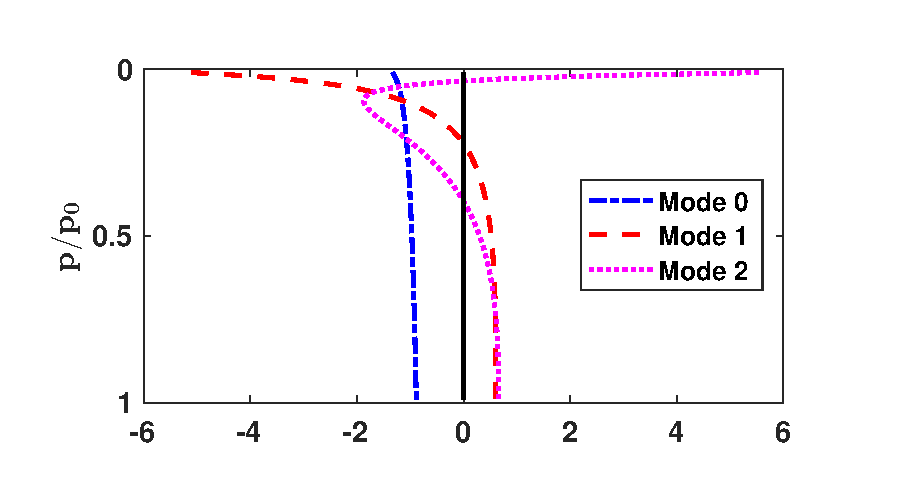
\includegraphics[scale=1]{./Chapter2/img/normalmodes}
\caption{The first three normal modes computed numerically. The equivalent depths are $h_0 = 9400$ m, $h_1 = 1270$ m, and $h_3 = 464$ m. The basic state $\tilde{\Gamma}(p)$ is given by equation (\ref{eq:staticstability}).}
\label{fig:normalmodes}
\end{figure}

The vertical modes are well resolved for most of the first 20. Beyond that, issues with under-resolving the modes start to appear. However, the issues resolving the modes appears to be located near the upper boundary, where the flow velocities are small (see Chapter \ref{ch:ch3}). Additionally, most of the energy is contained in the first several vertical modes (see Figures \ref{fig:modal_energy} and \ref{fig:modal_energy_nobaro}). The numerically computed modes still satisfy the orthonormality condition, and so energy from the more energetic modes do not contaminate the higher modes. Table \ref{tab:equivDepths} shows the computed equivalent depths for the first 30 vertical modes as well as the ratio $f/c_n$ (both dimensional and dimensionless), where $c_n = \sqrt{gh_n}$, which will be further discussed in Chapters \ref{ch:ch4} and \ref{ch:ch5}. For conciseness, only the odd numbered modes are shown. \\

\begin{table}
\begin{center}
\begin{tabular}{c c c c}

\hline
Vertical Mode & $h_n$ (m) & $\dfrac{f}{c_n}$ ($\mathrm{m}^{-1}$) & $\dfrac{L_x}{2\pi} \dfrac{f}{c_n}$\\
\hline\\
1 & 1582 & $8.02\cdot 10^{-7}$ & 0.65\\
3 & 306 & $1.82\cdot 10^{-6}$ & 1.5\\
5 & 107 & $3.09\cdot 10^{-6}$ &  2.5\\
7 & 50.9 & $4.48\cdot 10^{-6}$ & 3.6 \\
9 & 28.7 & $5.96\cdot 10^{-6}$ & 4.9 \\
11 & 18.0 & $7.52\cdot 10^{-6}$ & 6.1 \\
13 & 12.2 & $9.15\cdot 10^{-6}$ & 7.5\\
15 & 8.6 & $1.09\cdot 10^{-5}$ & 8.9\\
17 & 6.4 & $1.26\cdot 10^{-5}$ & 10.3\\
19 & 4.9 & $1.45\cdot 10^{-5}$ & 11.8\\
21 & 3.8 & $1.64\cdot 10^{-5}$ & 13.4\\
23 & 3.0 & $1.84\cdot 10^{-5}$ & 15.0\\
25 & 2.4 & $2.04\cdot 10^{-5}$ & 16.6\\
27 & 2.0 & $2.25\cdot 10^{-5}$ & 18.3\\
29 & 1.7 & $2.47\cdot 10^{-5}$ & 20.1\\
\hline
\end{tabular}
\end{center}
\caption{Equivalent depths and the ratio $f/c_n$ for odd numbered vertical modes between 1 and 30.}
\label{tab:equivDepths}
\end{table} 
\section{Solving the Horizontal Problem}
\label{sec:horiz}
Now that the vertical structure problem has been solved for vertical structure functions $Z_n(p)$ with corresponding eigenvalues $1/gh_n$, the horizontal structure problem defined by equations (\ref{eq:nmHorizBegin} - \ref{eq:nmHorizEnd}) is complete. This is recognized as the rotating shallow water $f$-plane equations, and so we proceed as outlined by Warn \cite{Warn1986a}. We assume the velocity and geopotential fields have a harmonic time dependence. That is, we further decompose (\ref{eq:separationBegin} - \ref{eq:separationEnd}) into
\begin{align}
&U(x,y,t) = \overline{U}(x,y) \exp{\left(-i \sigma t \right) }, \label{eq:harmonicBegin}\\
&V(x,y,t) = \overline{V}(x,y) \exp{\left(-i \sigma t \right) },\\
&\Phi^*(x,y,t) = \overline{\Phi}(x,y) \exp{\left(-i \sigma t \right)}. \label{eq:harmonicEnd}
\end{align}
Note that the bars do not refer to the complex conjugate here. From this point on the bars are also dropped for simplicity, understanding that $U$, $V$, and $\Phi$ are now functions of $(x,y)$ only. Substituting this into (\ref{eq:separationBegin} - \ref{eq:separationEnd}) results in 
\begin{align}
-i\sigma U - fV + \frac{\partial \Phi}{\partial x} &= 0,\\
-i\sigma V + fU + \frac{\partial \Phi}{\partial y} &= 0,\\
\frac{\partial U}{\partial x} + \frac{\partial V}{\partial y} - \frac{i\omega}{gh_n} \Phi &= 0.
\end{align}

If the domain has doubly-periodic boundary conditions, a natural basis to choose is a Fourier basis in the horizontal. The shallow water equations can then be written as

\begin{align}
-i\sigma \widehat{U} - f\widehat{V} + ik\widehat{\Phi} &= 0, \label{eq:shallowBegin}\\
-i\sigma \widehat{V} + f\widehat{U} + il\widehat{\Phi} &= 0,\\
ik\widehat{U} + il\widehat{V} - \frac{i\sigma}{gh_n} \widehat{\Phi} &= 0, \label{eq:shallowEnd}
\end{align}
where $\widehat{f}$ represents the Fourier transform of the field $f$ and $k$, $l$ represent the wavenumbers in the $x$- and $y$- directions, respectively. This results in another eigenvalue problem given by
\begin{align}
\sigma \left(\begin{array}{c}
\widehat{U}\\
\widehat{V}\\
\widehat{\eta}
\end{array}\right)=\left(\begin{array}{ccc}
0 & if & kc_n\\
-if & 0 & lc_n\\
kc_n & lc_n & 0
\end{array}\right)
\left(\begin{array}{c}
\widehat{U}\\
\widehat{V}\\
\widehat{\eta}
\end{array}\right) ,\label{eq:horizEigenvalue}
\end{align}
where $c_n = \sqrt{gh_n}$ and the geopotential has been scaled as $\eta = \Phi/c_n$ to make the matrix in equation (\ref{eq:horizEigenvalue}) Hermitian. By making this matrix Hermitian, the eigenvectors are guaranteed to be orthogonal for non-repeating eigenvalues, in addition to being complete.\\

This eigenvalue problem has eigenvalues and eigenvectors given by

\begin{align}
\sigma^0_{k,l,n} = 0, \quad &\mathbf{E}^0_{k,l,n} = \frac{1}{\sqrt{c^2_n K^2 + f^2}} \left(\begin{array}{c}
-ic_nl\\
ic_nk\\
f\end{array}\right),\label{eq:geo}\\[2ex]
\sigma^\pm_{k,l,n} = \pm \sqrt{c^2_nK^2 + f^2}, \quad &\mathbf{E}^0_{k,l,n} = \frac{1}{\sqrt{2}K\sqrt{c^2_n K^2 + f^2}} \left(\begin{array}{c}
ifl \pm k\sqrt{c^2_n K^2 + f^2}\\
-ifk \pm \sqrt{c^2_n K^2 + f^2}\\
c_nK^2\end{array}\right),\label{eq:ageo}
\end{align}
where $K^2 = k^2 + l^2$. The non-zero eigenvalues, $\sigma = \pm \sqrt{c^2_nK^2 + f^2}$ and its associated eigenvectors, give the dispersion relation for left- and right-traveling Poincar\'e waves. These are inertia gravity wave modes. 

\subsection{Geostrophic Motion}
\label{sec:geostrophicMotion}
From earlier, the separation of the system of equations (\ref{eq:nmHorizBegin} - \ref{eq:nmHorizEnd}) into vertical and horizontal structure is only valid for non-zero divergence. Another issue arises when $\partial \Phi^*/\partial t = 0$, i.e.\ when $\sigma = 0$. For the $\sigma = 0$ eigenvalue , we go back to the original separation of vertical structure from horizontal structure (\ref{eq:separationBegin}- \ref{eq:separationEnd}) and get 

\begin{align}
&V = \frac{1}{f} \frac{\partial \Phi^*}{\partial x},\label{eq:geoVertBegin}\\
&U = -\frac{1}{f} \frac{\partial \Phi^*}{\partial y},\\
&0 = \left(\frac{\partial U}{\partial x} + \frac{\partial V}{\partial y}\right),\label{eq:geoVertEnd}
\end{align}

i.e.\ geostrophic balance in the horizontal. For this reason, $\sigma^0_{k,l,n} = 0$, with its associated eigenvector in equation (\ref{eq:geo}), is the geostrophic mode. Note that in the geostrophic mode the vertical structure is unconstrained, and so we simply choose the same vertical structure as in the inertia-gravity wave modes. Since the vertical structure is the same, we have $c_n$ appearing in the geostrophic state as well.

\section{Energetics of the Horizontal and Vertical Decompositions}
By first solving the vertical eigenvalue problem to get appropriate vertical normal modes each corresponding to a unique $c_n$, each vertical mode reduces to a shallow water eigenvalue problem. The important thing to note is that because the eigenfunctions to the S-L problem (\ref{eq:nmVert}) with boundary conditions (\ref{eq:BCbot}) and (\ref{eq:BCtop}) are orthonormal, we can project any field $f$ onto the $m^{th}$ vertical mode $Z_m(p)$ by 
\begin{align}
f_m = \frac{1}{p_s} \int_0^{p_s} f(p) Z_m(p) ~\text{d}p,
\end{align}
and we can recover $f(p)$ by 
\begin{align}
f(p) = \sum_{m=0}^{\infty} f_m Z_m(p) .\label{eq:reconstruction}
\end{align}

In addition to the vertical modes being orthonormal, the shallow water system is Hermitian with distinct eigenvalues, which means that the eigenvectors in (\ref{eq:geo}) and (\ref{eq:ageo}) form an orthonormal basis as well. For a specific $c_n$, the projections of the Fourier coefficients of the velocity and scaled geopotential fields can be recovered in full by

\begin{align}
\left(\begin{array}{c}
\widehat{U}_n\\
\widehat{V}_n\\
\widehat{\eta}_n\end{array}\right)=
\sum_{k,l} A^0_{k,l,n} \mathbf{E}^0_{k,l,n} + A^+_{k,l,n} \mathbf{E}^+_{k,l,n} + A^-_{k,l,n} \mathbf{E}^-_{k,l,n},
\end{align}

where $A^0_{k,l,n}$ and $A^\pm_{k,l,n}$ refer to the amplitudes of the geostrophic and ageostrophic components for a specific $(k,l,n)$. The amplitudes can be determined by 
\begin{align}
A^0_{k,l,n} = \left(\begin{array}{c}
\widehat{U}_{k,l,n}\\
\widehat{V}_{k,l,n}\\
\widehat{\eta}_{k,l,n}\end{array}\right) \cdot \mathbf{E}^0_{k,l,n} = \frac{ic_nk\widehat{V}_{k,l,n} - ic_n \widehat{U}_{k,l,n} + f\widehat{\eta}_{k,l,n}}{\sqrt{c^2_nK^2 + f^2}}, \label{eq:amplitudes}
\end{align}
and similarly for $A^\pm_{k,l,n}$.\\

Consider a single wavevector $\mathbf{k} = (k, l)$ along with a single vertical mode number $n$. The first thing to note is the three regimes of motion that are possible:

\begin{itemize}
\item[] \textbf{Case 1:} $n = 0$, slow varying, nearly-constant vertical structure (see Figure \ref{fig:normalmodes}). This is the barotropic mode.
\item[] \textbf{Case 2:} $(k,l) = (0,0)$, there is no horizontal variation.
\item[] \textbf{Case 3:} $(k,l) \neq (0,0)$ and $n \neq 0$, the baroclinic modes.
\end{itemize}

Of these three, since this thesis is focused mainly on the mesoscale shallowing of the energy spectrum, case 2 (which corresponds to the mean flow), will be ignored moving forward.\\

The energy in the $n^{th}$ vertical mode can be related to the complex coefficients by Parseval's theorem,

\begin{align}
\begin{split}
E_n &= \frac{1}{L_x L_y} \left[ \iint ( (u_n)^2 + (v_n)^2) ~\text{d}\mathbf{x}  + \iint (\eta_n)^2 ~\text{d}\mathbf{x} \right]  = \\
&\quad\quad\quad \frac{1}{N_x N_y} \sum_{k,l} (|\widehat{U}_{k,l,n}|^2 + |\widehat{V}_{k,l,n}|^2) + \frac{1}{N_x N_y} \sum_{k,l} |\widehat{\eta}_{k,l,n}|^2.
\end{split}
\end{align}
To look at the energy spectra, consider a single $(k,l,n)$. The energy can be expressed in terms of the modal amplitudes by
\begin{align}
E_{k,l,n} = \frac{1}{2} \left( |\widehat{U}_{k,l,n}|^2 + |\widehat{V}_{k,l,n}|^2 \right) + \frac{1}{2} \left(|\widehat{\eta}_{k,l,n}|^2 \right) = \frac{1}{2} \left( |A^0_{k,l,n}|^2 + |A^+_{k,l,n}|^2 + |A^-_{k,l,n}|^2 \right).\label{eq:energyDecomp}
\end{align}

This energy can be binned by constant  constant circles in the $k$-$l$ plane with radius $|\mathbf{k}|$, where the energy at a horizontal wavelength $\mathbf{k}_h$ can be written as (e.g. \cite{Waite2004})
\begin{align}
E(\mathbf{k_h}) = \frac{1}{\Delta k} \sum_{k_h - \Delta k/2 < k' < k_h + \Delta k/2} E(\mathbf{k'}), \label{eq:binning}
\end{align}
where $\Delta k = 2\pi/L_x$. By binning the energy this way, information about the anisotropy of the flow is lost. However, this circular binning technique employed here serves only as an example diagnostic. The normal mode theory developed here does not require flows to be isotropic, and it would also be possible to look at one-dimensional spectra in the zonal or meridional directions, if desired.

In addition, due to the orthonormality condition (\ref{eq:reconstruction}), the modal amplitudes can be summed to give
\begin{align}
A^0_{k,l} = \sum_{n=0}^\infty A^0_{k,l,n},
\end{align}
and similarly for $A^+_{k,l}$ and $A^-_{k,l}$. This provides a clean way to compare the total geostrophic and ageostrophic energy.

\section{Summary}

In this chapter, the linear normal mode theory for decomposing the flow into geostrophic and ageostrophic components was developed. Through the orthonormality of the decomposition together with the completeness of the eigenfunctions, this decomposition allows us to to relate the spectral coefficients, $(\widehat{U},\widehat{V}, \widehat{\eta})$, to  the geostrophic and ageostrophic amplitudes by equation (\ref{eq:energyDecomp}). Through Parseval's theorem, these spectral coefficients can be related to the kinetic and potential energy in physical space. Combining these two results, we can therefore take the energy contained in a flow and represent it in terms of the geostrophic and ageostrophic motion.\\

In the next chapter, we apply this normal mode decomposition to a baroclinic instability simulation of a double jet. Details of the simulation, including initialization procedures, are discussed  and the evolution of the jet as it breaks down is presented to give the reader an intuitive understanding of the study.
\chapter{Numerical Simulation of a Baroclinic Life Cycle}
\label{ch:ch3}
\section{Analytic Initial Conditions for a Double Jet}
As outlined in Chapter \ref{ch:ch1}, baroclinic instabilities are of interest to researchers for many reasons; for example, the resulting weather patterns baroclinic wave life cycles give rise to. To study a jet in a channel, one of the common initialization techniques is to prescribe a small, zonally invariant potential vorticity (PV) in the troposphere combined with a larger (usually by an order of magnitude)  PV in the stratosphere (e.g.\  \cite{Zhang2004}, \cite{Plougonven2007}, \cite{Waite2009}).  To represent the tropopause, a function with a sharp gradient (e.g.\ hyperbolic tangent function) can be used to separate the troposphere and the tropopause. The initial velocity field can then be recovered by iteratively inverting the PV (e.g\ \cite{Plougonven2007}). Instead of this iterative procedure, it can be advantageous to have an analytic initial conditions for multiple reasons. For example, by referring to the vertical structure problem in Section \ref{sec:normalModes}, the derivative of the static stability can be analytically written, removing the error that would be introduced from a numerical computation. Additionally, parameters can be adjusted to allow for different initial conditions, such as including a $\beta$-plane or adding moisture.\\

 However, creating initial fields for an analytic jet is not a trivial task, as the jet must be a steady-state solution to the governing equations and must also contain strong vertical shear in order to create baroclinic instability in the atmosphere. It is for this reason that we take a modified approach to the jet in a channel presented in a 2015 paper by Ullrich, Reed, and Jablonowski (hereafter referred to as URJ15) \cite{Ullrich2015}. This jet is formulated to initially be in hydrostatic, geostrophic, and thermal wind balance in a 3-D channel. In addition, URJ15 develop the initial conditions in $\eta = p/p_0$ coordinates, consistent with the normal mode formulation of Chapter \ref{ch:ch2}. In this section, the setup of the (single) zonal jet in a 3-D channel by URJ15 is presented, as well as the modifications made to transform the jet into a double jet in a doubly-periodic domain.

\subsection{Velocity Field in a Channel}
The initial velocity field consists of a zonal wind given by 
\begin{align}
u(x,y,\eta) = -u_0 \sin^2 { \left(\frac{\pi y}{L_y}\right)} \ln{\eta} \exp{\left\{-\left(\frac{\ln \eta}{b}\right)^2\right\}}.
\end{align}
Here $u_0$, $L_y$, and $b$ are tunable physical parameters. Refer to Table \ref{tab:parameters} for specific parameters used in the simulations for this thesis. Note that the zonal velocity field is independent of $x$, as one would expect for a zonal jet.\\


The prescribed zonal velocity field has several desirable features. The meridional-varying part ensures the zonal velocity goes to 0 at the boundaries $y = 0, L_y$, while the pressure-dependent part ensures that the velocity approaches 0 at both the surface and model top. It can be shown that the velocity reaches a maximum value at around 240 hPa, which is close to the observations of mid-latitude jets \cite{Ullrich2015}. One important thing to note is that the parameter $u_0$ does not actually set the maximum velocity. In fact, the true maximum lies at a value slightly less than this parameter. \\

\begin{table}[H]
\centering
\begin{tabular}{|c|l|l|}
\hline
\textbf{Parameter} & \textbf{Description} & \textbf{Value} \\ \hline
$u_0$ & velocity scale factor for the jet & $55~\text{m s}^{-1}$ \\ \hline
$L_y$ & Channel width in meridional direction & $5120~\text{km}$ \\ \hline
$b$ & dimensionless vertical width parameter of jet & $ 2$ \\ \hline
$T_0$ & surface temperature & 288 K \\ \hline
$g$ & acceleration due to gravity &  $9.81~\text{m s}^{-1}$\\ \hline
$\Gamma$ & lapse rate & $0.005~\text{K m}^{-1}$\\ \hline
$R_d$ & ideal gas constant of dry air & $287 ~\text{J kg}^{-1} \text{K}^{-1}$ \\ \hline
$f_0$ & Coriolis parameter & $ 1.03 \times 10^{-4} ~\text{s}^{-1}$ \\ \hline
\end{tabular}
\caption{Parameters used in the initialization of the analytic jet.}
\label{tab:parameters}
\end{table}
The meridional velocity and vertical velocity are both set to 0 initially. From the initial velocity fields, it is trivially non-divergent (i.e.\ $\delta = 0$).\\

The vertical vorticity is likewise easy to compute, and can be represented by
\begin{align}
\zeta(x,y,\eta) = -\frac{\partial u}{\partial y} = \frac{2\pi u_0}{L_y} \sin{\left(\frac{\pi y}{L_y}\right)} \cos{\left(\frac{\pi y}{L_y}\right)} \ln{\eta} \exp{\left\{-\left(\frac{\ln \eta}{b}\right)^2\right\}}.
\end{align}

Figure \ref{fig:initialVelVort} shows a meridional-vertical cross section of the velocity and vertical vorticity fields of the jet.
\begin{figure}[H]
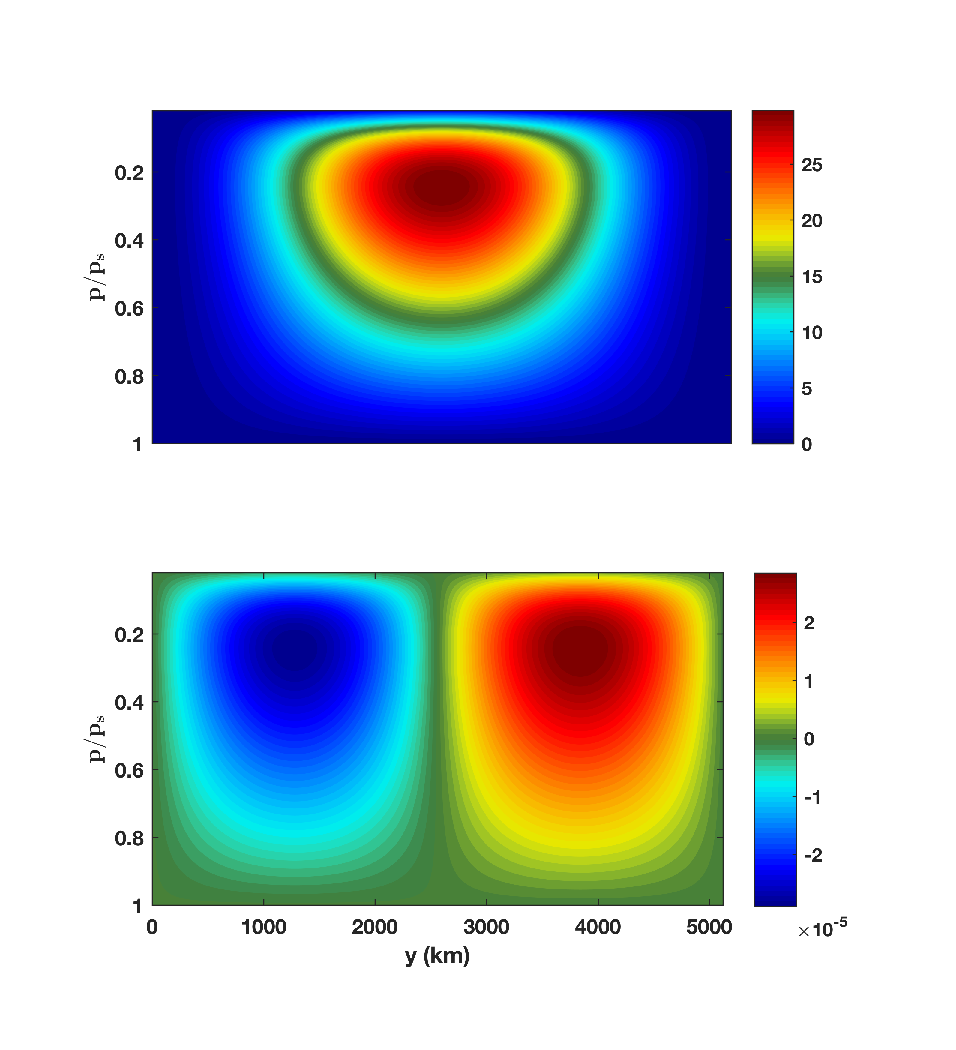
\includegraphics[scale=1]{Chapter3/img/initialVelVort}
\caption{Meridional slice of initial velocity (in m $\text{s}^{-1}$, top) and vertical vorticity (in $\text{s}^{-1}$, bottom) of the single jet.}
\label{fig:initialVelVort}
\end{figure}

\subsection{Geopotential and Temperature Fields in a Channel}

The geopotential field is prescribed by a horizontal-mean geopotential given by

\begin{align}
\left\langle\Phi(\eta)\right\rangle = \frac{T_0 g}{\Gamma}\left(1 - \eta^{\frac{R_d \Gamma}{g}}\right),
\end{align}

where $T_0$ is the surface temperature, $g$ is the acceleration due to gravity, $R_d$ is the ideal gas constant for dry air, and $\Gamma$ is the lapse rate of the atmosphere. Note that $\Gamma$ in this section is different from the static stability $\tilde{\Gamma}$ from Section \ref{sec:normalModes}. This is then combined with a spatially varying deviation of the geopotential from the horizontal mean in order to maintain geostrophic balance. The total geopotential, including the deviation from the horizontal-mean, on an $f$-plane is given by

\begin{align}
\Phi(x,y,\eta) =\left\langle\Phi(\eta)\right\rangle +  \Phi'(x,y)\ln{\eta} \exp{\left\{ -\left(\frac{\ln{\eta}}{b}\right)^2\right\}},
\end{align}
with $\Phi'(x,y)$ given by
\begin{align}
\Phi'(x,y) = \frac{u_0 f_0}{2}\left[y - \frac{L_y}{2} - \frac{L_y}{2\pi} \sin{\left(\frac{2\pi y}{L_y}\right)}\right] .
\end{align}
Here, $u_0$ is the same parameter as in the initial velocity field, and $f_0$ is the $f$-plane Coriolis paramter (approximately $10^{-4} ~\text{s}^{-1}$ at a latitude of $45\degree$). URJ15 provide a more complicated expression to allow for the possibility of a $\beta$-plane, but the normal mode theory from Chapter \ref{ch:ch2} focuses solely on the $f$-plane.\\

In addition to prescribing the velocity fields and geopotential field, a temperature field is required to completely describe the initial state of the jet. Similarly to the geopotential, the temperature field is composed of a horizontal-mean temperature field with a deviation from this base state. The horizontal-mean temperature is given by

\begin{align}
\left\langle T(\eta)\right\rangle = T_0 \eta^{\frac{R_d \Gamma}{g}}.
\end{align}

In order to be initially in hydrostatic balance, a deviation from the horizontal-mean temperature is given by

\begin{align}
T'(x,y,\eta) = \frac{\Phi'(x,y)}{R_d} \left\{ \frac{2}{b^2}(\ln {\eta})^2 - 1\right\} \exp{\left\{-\left(\frac{\ln{\eta}}{b}\right)^2\right\} }.
\end{align}

Figure \ref{fig:initialGeo} shows the initial geopotential field, while Figure \ref{fig:tempBuoy} shows the vertical profile of the stratification of the atmosphere proposed by URJ15. 

\begin{figure}[H]
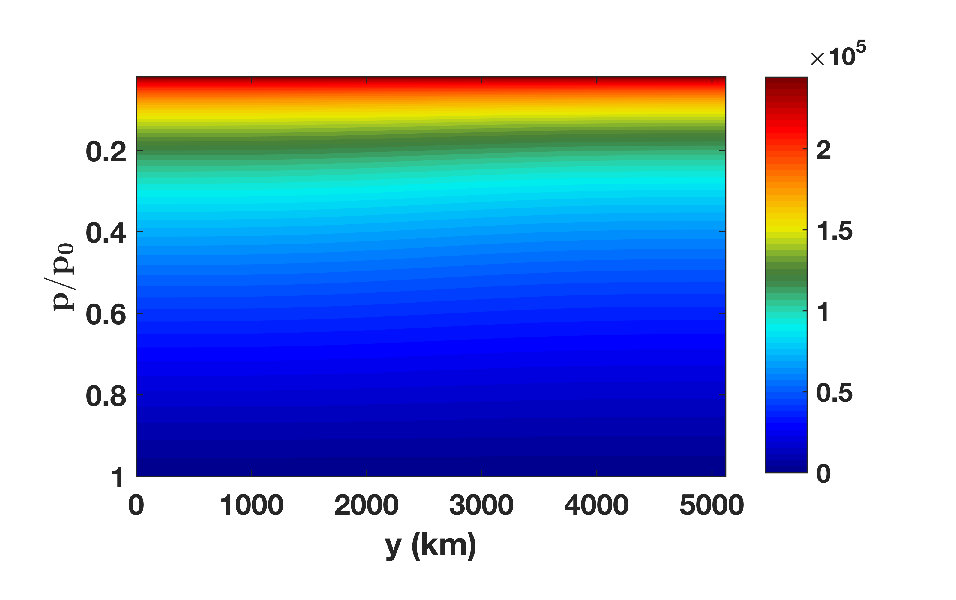
\includegraphics[scale=1]{Chapter3/img/initialGeo}
\caption{Meridional slice of the geopotential field ($\text{m}^2~\text{s}^{-2}$) for a single jet.}
\label{fig:initialGeo}
\end{figure}

Although the initial conditions for the atmosphere proposed by URJ15 notably lack a tropopause, the atmosphere is still stably stratified and the sharp increase in Br{\"u}nt-Vaisala frequency near the domain top helps to further reduce gravity wave reflections off of the lid.

\begin{figure}[H]
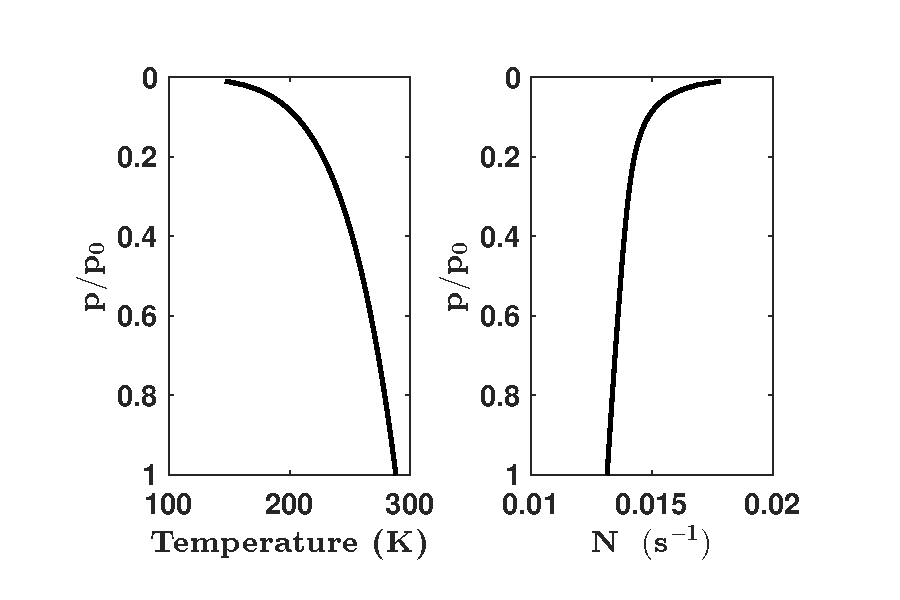
\includegraphics[scale=1]{Chapter3/img/tempBuoy}
\caption{Initial mean vertical profile of the horizontal mean temperature (left) and Brunt-V\"ais\"al\"a frequency (right).}
\label{fig:tempBuoy}
\end{figure}



\subsection{Extension From a Channel to a Doubly-Periodic Domain}
To take advantage of the Fourier transform in the meridional direction without involving the complicated boundary conditions for the normal mode decomposition that arise from a channel, we extend the analytic formulas presented by URJ15 to doubly-periodic domain while maintaining an initially balanced system.\\

The domain is extended from $y \in [0, L_y]$ to $y \in [-L_y, L_y]$. The geopotential and temperature fields are chosen to be even extensions about $y=0$. This choice is physically sensible as it maintains hydrostatic balance.\\

For the velocity fields, the meridional and vertical fields are still chosen to be 0, but the zonal velocity field must be altered to maintain geostrophic balance. Since $\Phi$ was evenly extended about $y=0$, $\partial \Phi/\partial y$ is odd about $y = 0$. We therefore require that the zonal velocity field be an odd extension about $y = 0$. A meridional slice of the geopotential in Figure \ref{fig:initialGeoDouble} and the initial velocity and vertical vorticity fields in Figure \ref{fig:initialVelVortDouble} show the new extended doubly-periodic domain with a double jet.\\

\begin{figure}[H]
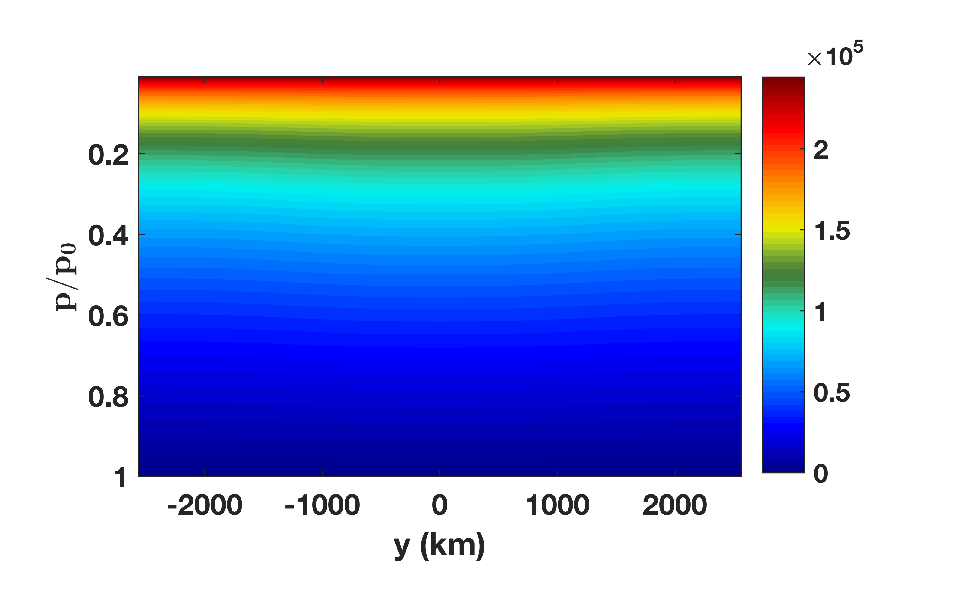
\includegraphics[scale=1]{Chapter3/img/initialGeoDouble}
\caption{Meridional slice of the initial geopotential ($\text{m}^2 ~\text{s}^{-2}$) after the domain has been extended to be doubly periodic.}
\label{fig:initialGeoDouble}
\end{figure}

\begin{figure}[H]
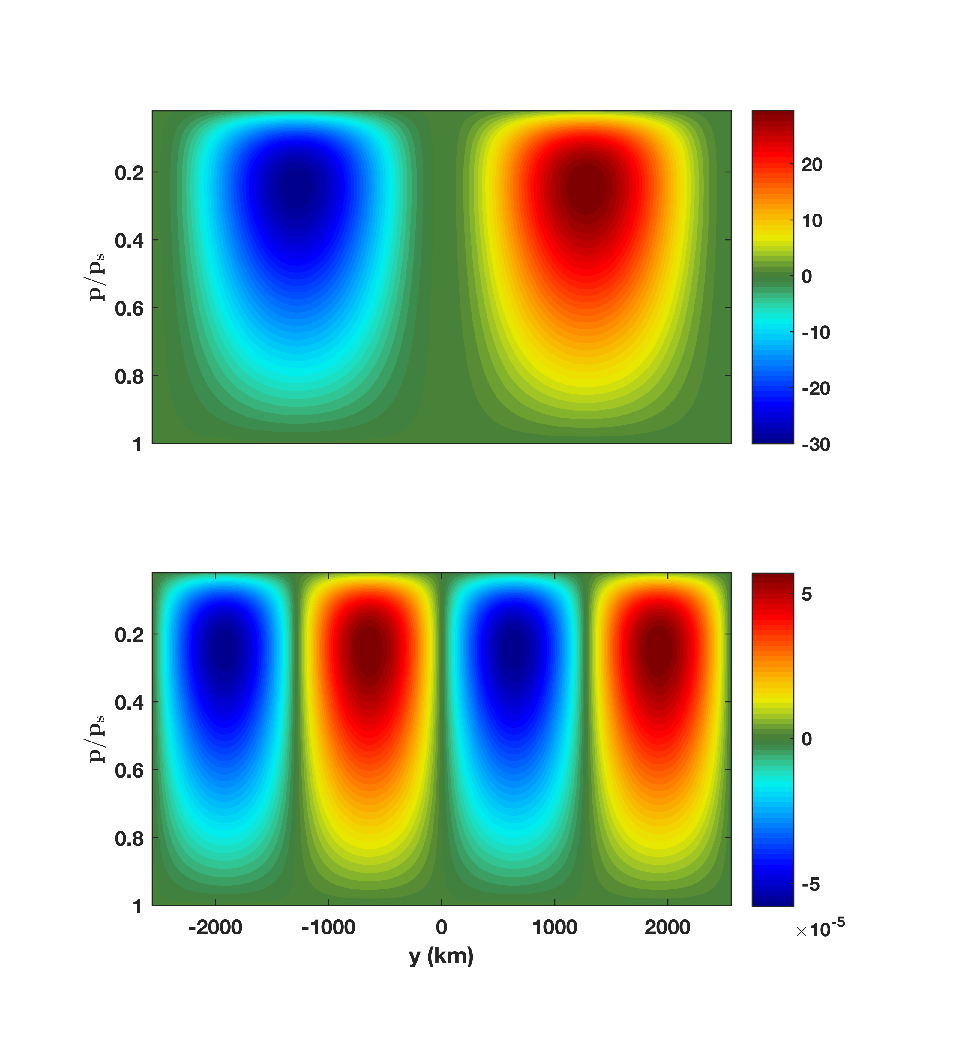
\includegraphics[scale=1]{Chapter3/img/initialVelVortDouble}
\caption{Meridional slice of initial velocity (top, in $\text{m s}^{-1}$) and vertical vorticity (bottom, in $\text{s}^{-1}$) after the domain has been extended to be doubly periodic.}
\label{fig:initialVelVortDouble}
\end{figure}
One final difference between the initial state presented in this thesis and in the initial state presented by URJ15 is the baroclinic wave triggering mechanism. URJ15 propose a Gaussian perturbation of the zonal velocity field. We choose to use a Gaussian perturbation of amplitude $4$ K  and root-mean-square width $600$ m to the potential temperature field, taking care to numerically recalculate the geopotential and density since the mass in the air column should not change, and we rebalance hydrostatically. Both approaches mean that the baroclinic jet is no longer in geostrophic balance, and high-speed gravity waves are triggered. URJ15 argue that the gravity waves are dampened by diffusion before the baroclinic life cycle begins, especially since the perturbation to the potential temperature field in our simulation is small.

\section{Model Choice and Simulation Overview}
\label{sec:simulationOverview}
To study the baroclinic life cycle, we employ the Weather Research and Forecasting model advanced research core (WRF-ARW) \cite{Skamarock2008}. WRF is a robust finite difference model with third order Runge-Kutta (RK3) time-split integration that solves the Euler equations. For the vertical coordinate, WRF uses a terrain-following, hydrostatic-pressure coordinate. It is non-hydrostatic, fully compressible, and the spatial discretization features $2^{nd}$ to $6^{th}$ order advection options. For this study, we use $5^{th}$ and $3^{rd}$ order horizontal and vertical advection, respectively. The odd-ordered schemes are upwind biased in WRF, adding numerical dissipation to the model. The WRF-ARW core is a parallelized model capable of running both real data simulations and idealized simulations. \\

Though WRF-ARW offers many physics options, including surface physics, cloud parameterizations, and microphysics, the work presented here is an idealized study. Therefore, the simulation is run without moisture, planetary boundary layer physics, surface physics, or radiation physics. No additional dissipation scheme is applied, as the numerical dissipation from the finite difference advection scheme does an adequate job of removing energy build up in the subgrid scale (discussed in Chapter \ref{ch:ch4}).\\

 The governing equations used by WRF are different from the linearized equations (\ref{eq:nmMomentum}-\ref{eq:nmThermo}) used to derive the normal mode theory. Though the model itself is non-hydrostatic, it uses a terrain-following pressure coordinate denoted by
\begin{align}
\eta = (p_h - p_{ht})/\mu \label{eq:wrfVert},
\end{align}
where $p_h$ is the hydrostatic pressure, $p_{ht}$ is the hydrostatic pressure at the model top, $\mu = p_{hs} - p_{ht}$ is the mass per unit area, and $p_{hs}$ is the hydrostatic pressure at the model surface. Note that this vertical coordinate is different from the $\eta$ coordinate used by URJ15. The dry WRF equations of motion following this pressure coordinate and written in flux-form are
\begin{align}
\frac{\partial U}{\partial t} + (\nabla \cdot \mathbf{V}u) - \frac{\partial p\Phi_eta}{\partial x} + \frac{\partial p\Phi_x}{\partial \eta} &= F_U,\label{eq:wrfXMomentum}\\
\frac{\partial V}{\partial t} + (\nabla \cdot \mathbf{V}v) - \frac{\partial p\Phi_eta}{\partial y} + \frac{\partial p\Phi_y}{\partial \eta} &= F_V, \label{eq:wrfYomentum}\\
\frac{\partial W}{\partial t} + (\nabla \cdot \mathbf{V}w) - g\left(\frac{\partial p}{\partial \eta} - \mu\right)& = F_W, \label{eq:wrfPMomentum}\\
\frac{\partial \Theta} {\partial t} + (\nabla \cdot \mathbf{V}\theta) &= F_\Theta, \label{eq:wrfThermo}\\
\frac{\partial \mu}{\partial t} + (\nabla \cdot \mathbf{V}) &= 0, \label{eq:wrfContinuity}\\
\frac{\partial \Phi}{\partial t} + \mu^{-1}\left[(\mathbf{V} \cdot \nabla \phi) - gW\right] &= 0, \label{eq:wrfGeopotential}
\end{align}
where $\mathbf{V} = \mu\mathbf{v}$, $\Theta = \mu\theta$, and $F_U$, $F_V$, $F_W$, and $F_\Theta$ represent the forcing terms from model physics, turbulent mixing, and Earth's rotation. Subscripts in equations (\ref{eq:wrfXMomentum} - \ref{eq:wrfYomentum}) represent partial derivatives. Equations (\ref{eq:wrfXMomentum} - \ref{eq:wrfContinuity}) are written in conservation form, while equation (\ref{eq:wrfGeopotential}) is not because $\mu\Phi$ is not a conserved quantity. For dry dynamics, the last thing WRF needs is a diagnostic equation for hydrostatic balance, given by
\begin{align}
\frac{\partial \Phi}{\partial \eta} + \frac{\mu}{\rho} = 0. \label{eq:wrfHydrostatic}
\end{align}
Note that the hydrostatic equation (\ref{eq:wrfHydrostatic}) does not constrain the solution, but instead is part of the vertical coordinate definition. The pressure, $p$, and hydrostatic pressure, $p_h$, are stored as two different state variables in the WRF model.\\

We use a moderate-resolution domain with a size of 1024x1024x100  points.  WRF uses an Arakawa C-grid \cite{Arakawa1977}, which staggers certain variables such as velocities to cell edges, while other variables such as geopotential, air mass columns, and potential temperature among others are kept at cell centers or ``mass points''. Refer to Figure \ref{fig:Cgrid} for an example layout of the Arakawa C-grid. This means that our zonal velocity field is actually $1025 \times 1024 \times 100$ points, the meridional velocity is $1024 \times 1025 \times 100$ points, and the vertical velocity its $1024 \times 1024 \times 101$ points. We use periodic boundary conditions in the horizontal. In the vertical, the free slip boundary condition is used at the bottom, while a constant pressure level at the top boundary along a material surface is combined with diffusive damping starting 5000 m from the top to reduce gravity wave reflections. \\
\begin{figure}[H]
\begin{center}
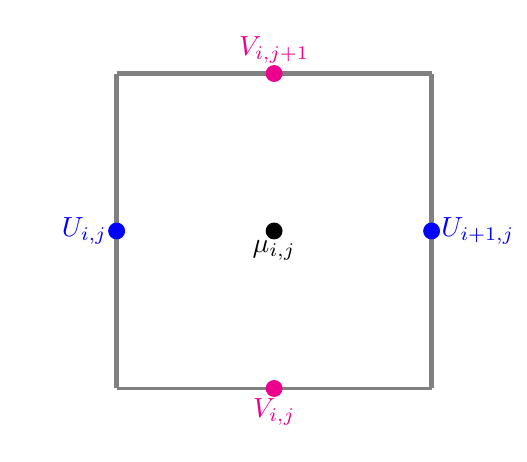
\begin{tikzpicture}
\draw[gray, ultra thick] (-2,-2) -- (-2,2);
\draw[gray, ultra thick] (-2,2) -- (2,2);
\draw[gray, ultra thick] (2,2) -- (2,-2);
\draw[gray, very thick] (2,-2) -- (-2,-2);

\filldraw[blue] (2,0) circle (0.1) node[anchor=west] {$U_{i+1,j}$};
\filldraw[blue] (-2,0) circle (0.1) node[anchor=east] {$U_{i,j}$};
\filldraw[magenta] (0,-2) circle (0.1) node[anchor=north] {$V_{i,j}$};
\filldraw[magenta] (0,2) circle (0.1) node[anchor=south] {$V_{i,j+1}$};
\filldraw[black] (0,0) circle (0.1) node[anchor=north] {$\mu_{i,j}$};
\end{tikzpicture}
\caption{An example of state variable positioning on a single cell in the Arakawa C-grid. This view is of a horizontal level (i.e.\ no vertical indices are shown, though vertical staggering is identical for the vertical velocity $w$). Here $A_{i,j}$ represents the $i^{th}$ row and the $j^{th}$ column of state variable $A$. Zonal and meridional velocities are staggered in the $x$- and $y$-directions, respectively. An example of a state variable stored at mass points is $\mu$, the mass per unit area in the air column.}
\label{fig:Cgrid}
\end{center}
\end{figure}

Our simulation uses a moderate resolution grid spacing of $\Delta x = \Delta y = 5~\text{km}$ in the horizontal, with $\Delta p \approx 10 ~\text{mbar}$ in the vertical. This corresponds to a domain size of $L_x = L_y = 5 120$ km in the horizontal and $L_z \approx 25$ km in the vertical. Since the grid is evenly spaced in $p$, the grid spacing in $z$ changes throughout the domain. $\Delta z$ near the surface is approximately $170$ m, while $\Delta z$ near the top is approximately $2000$ m. The time step is chosen to be $\Delta t = 30$ seconds for numerical stability reasons. The simulation is run for 15 days in model time, allowing sufficient time for the baroclinic instabilities to grow and saturate. During this time, a number of common mesoscale phenomena appear, such as surface fronts shown in Figure \ref{fig:frontSquall}. Kelvin-Helmholtz instabilities and PV spirals are commonly seen along these fronts \cite{Plougonven2013,Methven1998}.  Figure \ref{fig:vortTimeSeries} shows the vertical vorticity, $\zeta = \partial V/\partial x -\partial U/\partial y$, at a height of roughly 250 hPa over the course of the simulation. Figure \ref{fig:div} shows the horizontal divergence at this same height and times as in Figure \ref{fig:vortTimeSeries}. To better understand the motion, we also examine the divergence and vorticity at different heights. Figures \ref{fig:vort_height_25} and \ref{fig:vort_height_50} show the vertical vorticity time series taken during the same days as in Figure \ref{fig:vortTimeSeries}, but at heights of 750 hPa and 500 hPa, respectively. Figures \ref{fig:div_height_25} and \ref{fig:div_height_50} show the horizontal divergence during the same days as in \ref{fig:div}, but at heights of 750 hPa and 500 hPa, respectively. Together, the vertical vorticity and horizontal divergence in the figures show the rotational and divergent components of the Helmholtz decomposition at that specific height and can help the reader to visualize the Helmholtz decomposition.
\\
\begin{figure}[H]
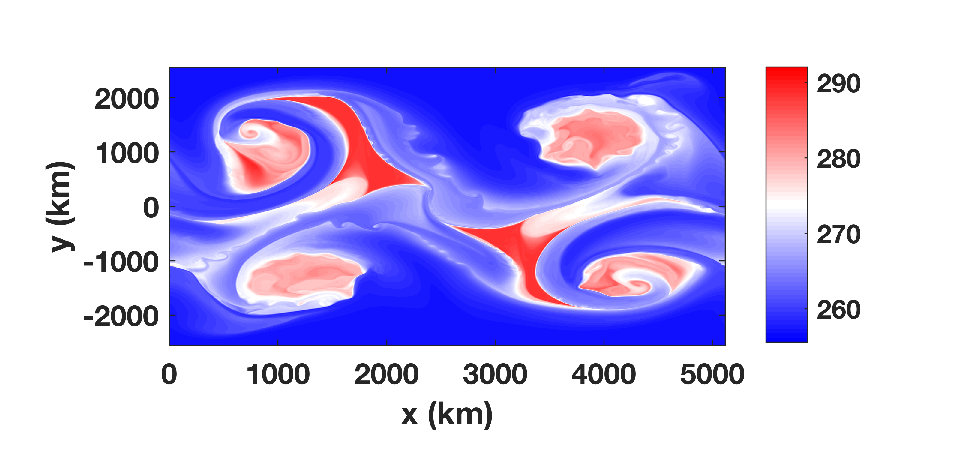
\includegraphics[scale=1]{Chapter3/img/front}
\end{figure}
\begin{figure}[H]
\vspace{-1em}
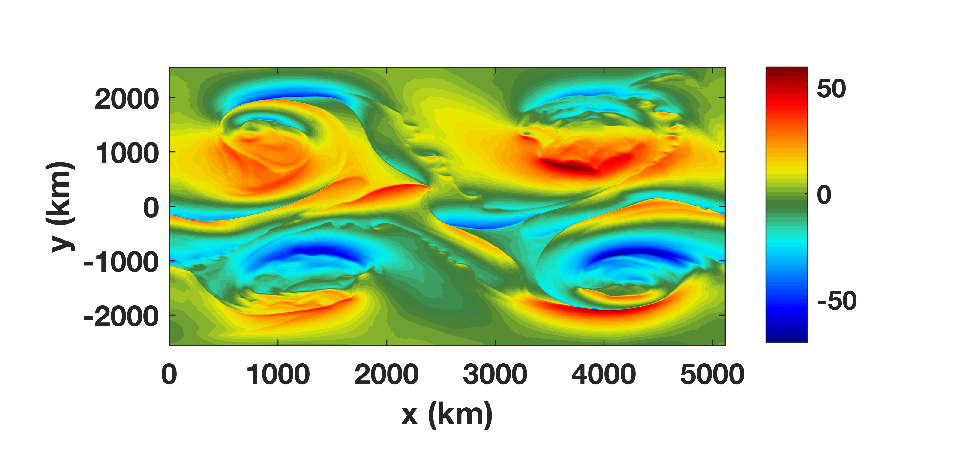
\includegraphics[scale=1]{Chapter3/img/squall}
\caption{Temperature (K, top) and zonal velocity (m $\text{s}^{-1}$, bottom) show cold and warm fronts at the surface.}
\label{fig:frontSquall}
\end{figure}
\vspace{-2em}
\begin{figure}[H]
\vspace{-3em}
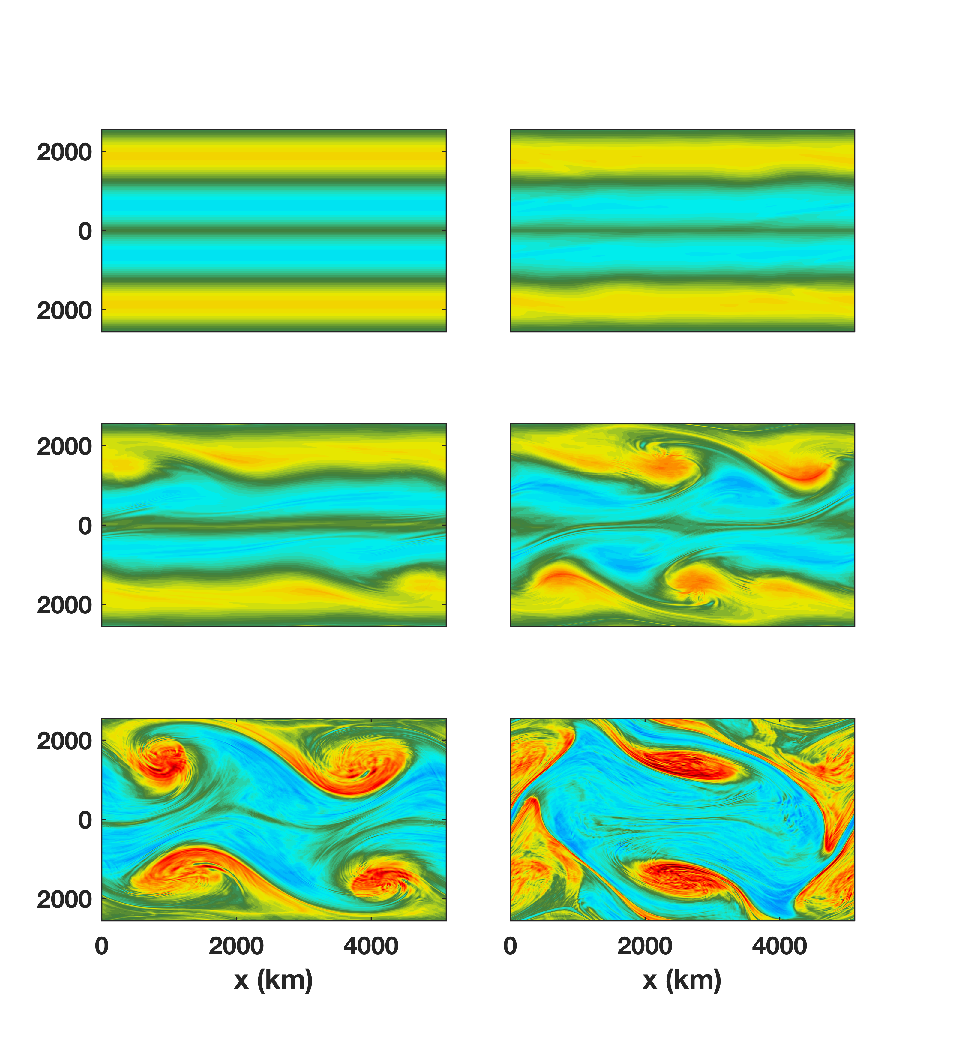
\includegraphics[scale=1]{Chapter3/img/vortTimeSeries}
\caption{Snapshots of the vertical vorticity at a height of roughly 300 hPa at different points in time. The top row shows day 0 (top left) and day 2 (top right). The middle row shows day 5 (middle left) and day 8 (middle right). The bottom row shows day 11 (bottom left) and day 14 (bottom right). The color map has units of $f$, ranging from $-2f$ to $2f$. There are peak values of around $\pm 2.5f$ in days 11 and 14.}
\label{fig:vortTimeSeries}
\end{figure}


\begin{figure}[H]
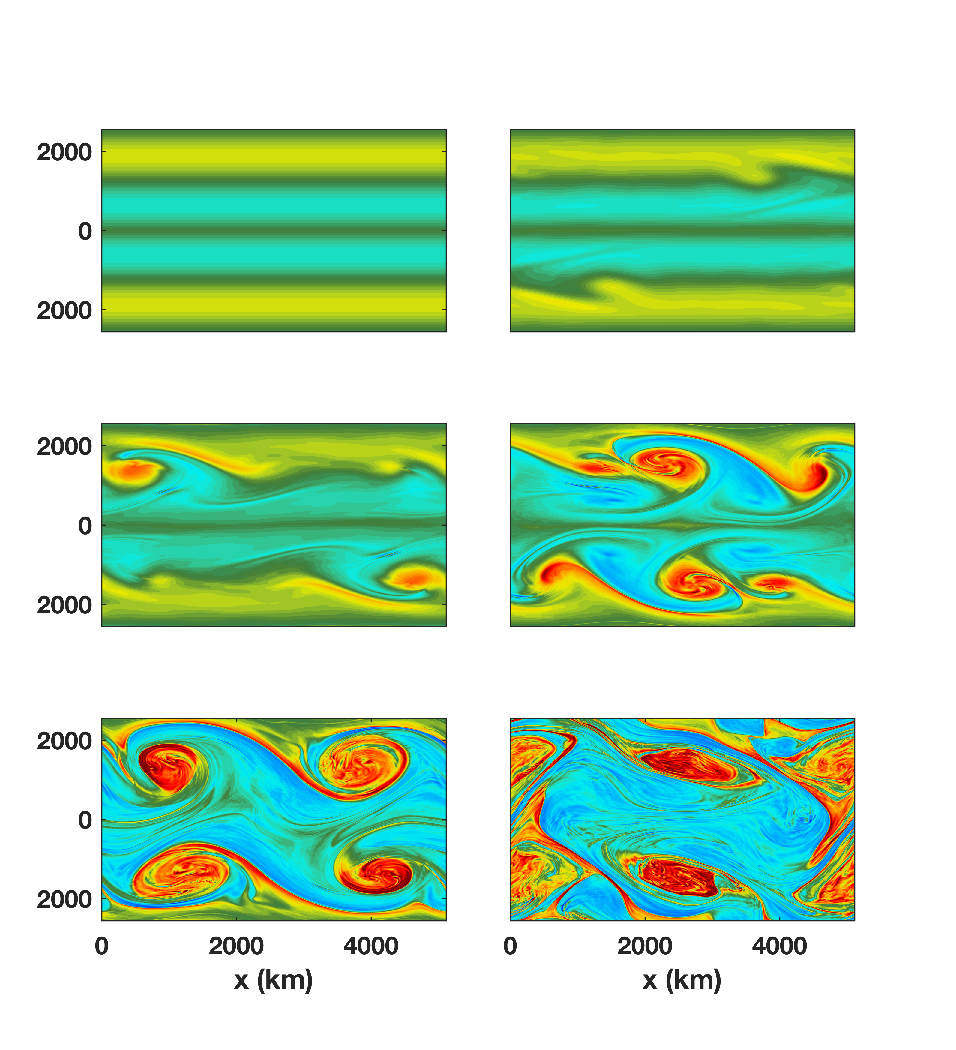
\includegraphics[scale=1]{Chapter3/img/vort_height_50}
\caption{As in Figure \ref{fig:vortTimeSeries}, but at a height of 500 hPa.}
\label{fig:vort_height_25}
\end{figure}

\begin{figure}[H]
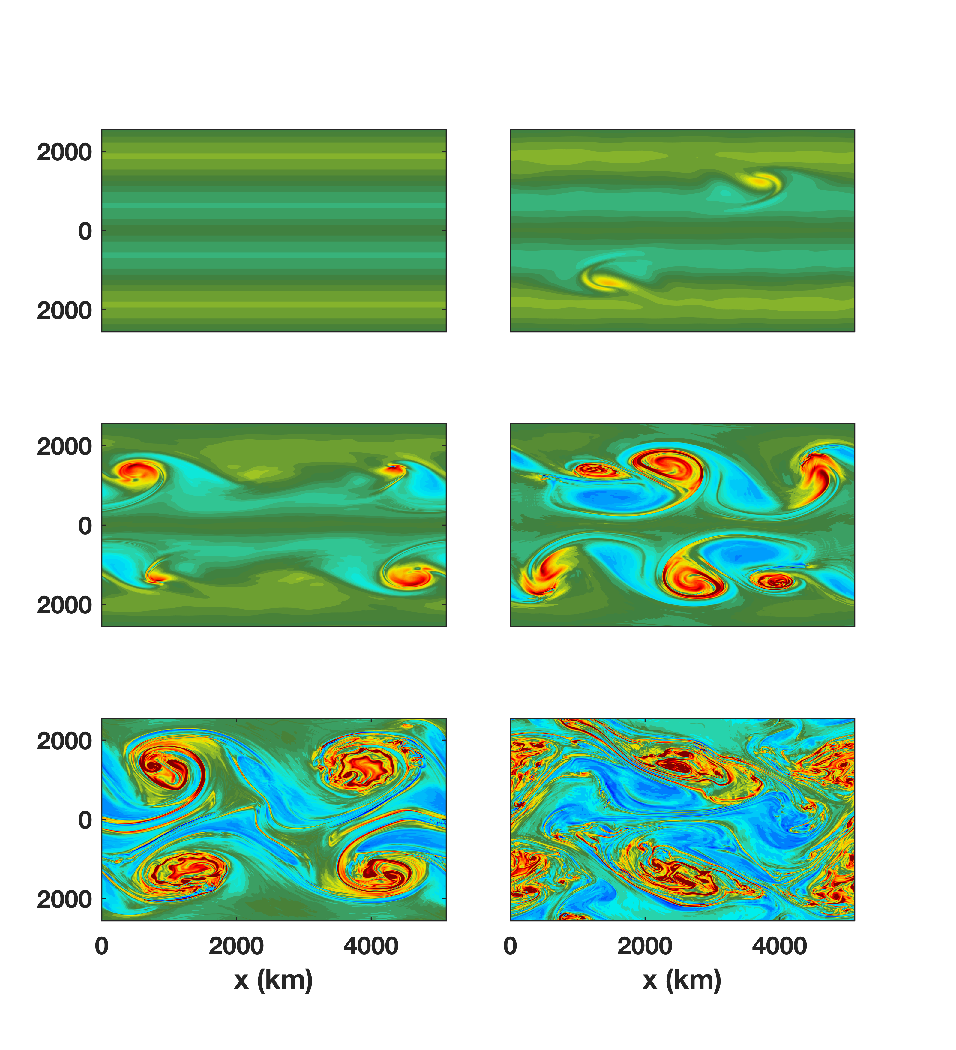
\includegraphics[scale=1]{Chapter3/img/vort_height_25}
\caption{As in Figure \ref{fig:vortTimeSeries}, but at a height of 750 hPa.}
\label{fig:vort_height_50}
\end{figure}

\begin{figure}[H]
\vspace{-3em}
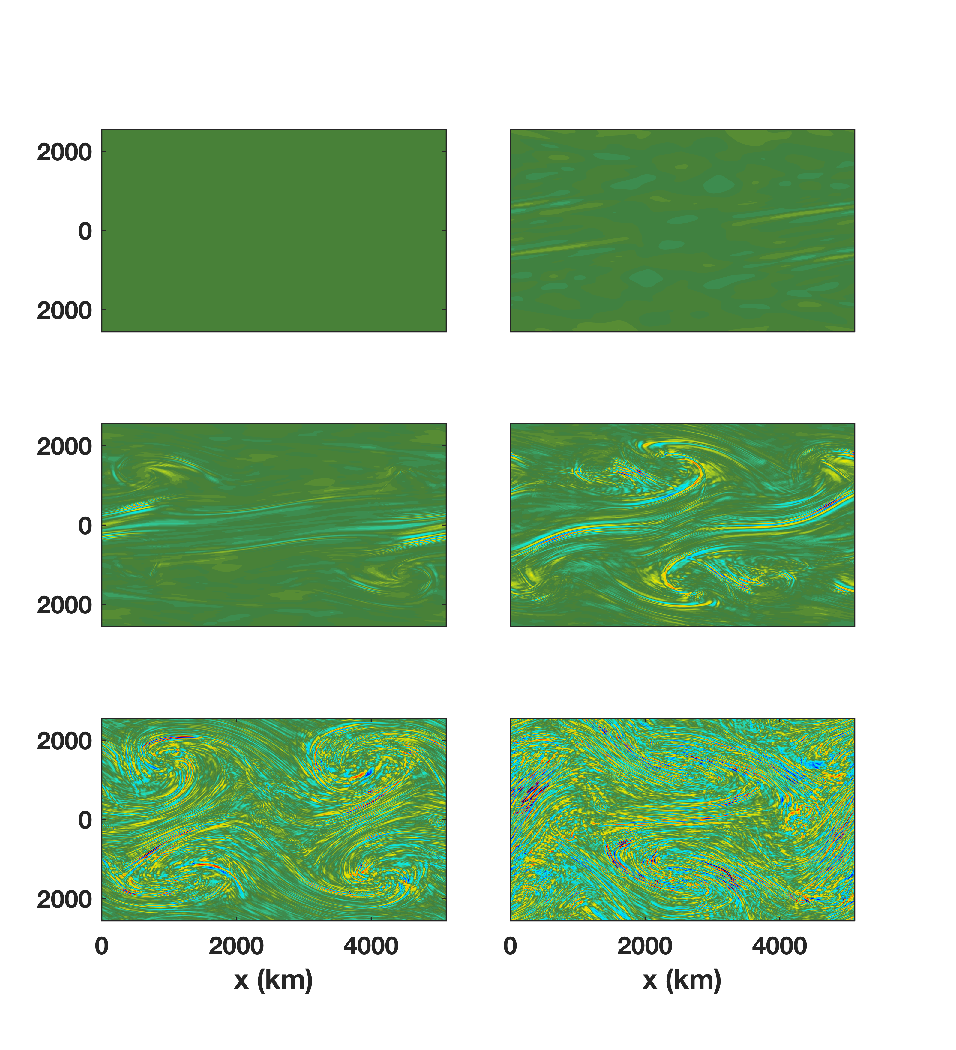
\includegraphics[scale=1]{Chapter3/img/div}
\caption{Snapshots of the horizontal divergence at a height of roughly 300 hPa at different points in time. The top row shows day 0 (top left) and day 2 (top right). The middle row shows day 5 (middle left) and day 8 (middle right). The bottom row shows day 11 (bottom left) and day 14 (bottom right). The color map has units of $f$, ranging from $-2f$ to $2f$.}
\label{fig:div}
\end{figure}

\begin{figure}[H]
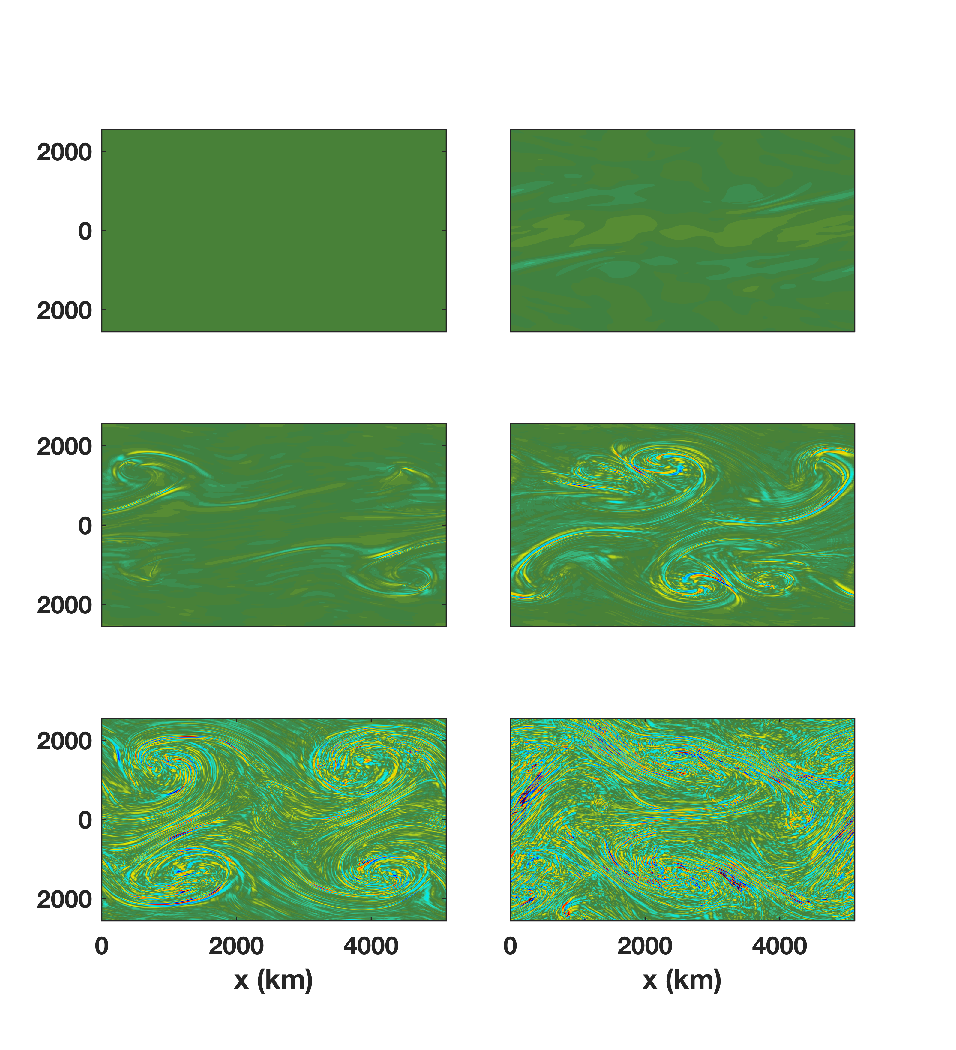
\includegraphics[scale=1]{Chapter3/img/div_height_50}
\caption{As in Figure \ref{fig:div}, but at a height of 500 hPa.}
\label{fig:div_height_25}
\end{figure}

\begin{figure}[H]
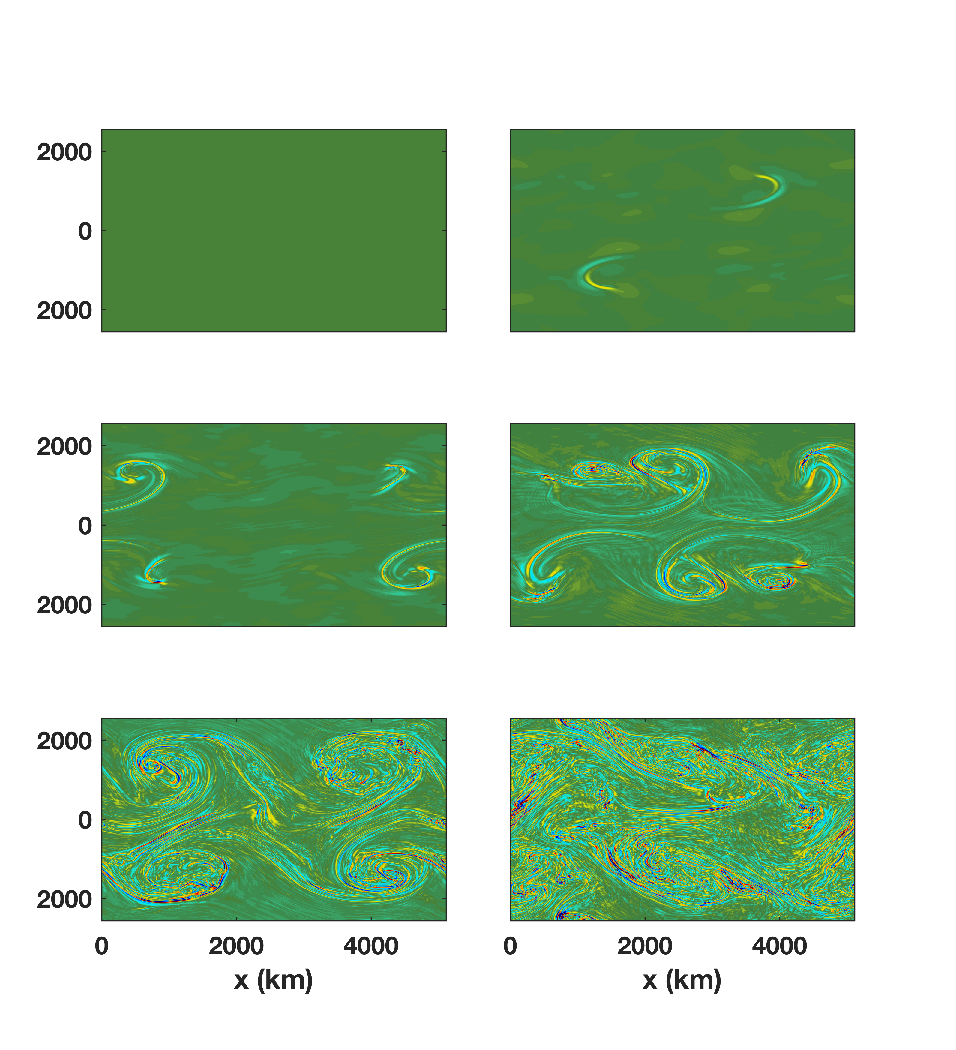
\includegraphics[scale=1]{Chapter3/img/div_height_25}
\caption{As in Figure \ref{fig:div}, but at a height of 750 hPa.}
\label{fig:div_height_50}
\end{figure}

To better understand the breaking of the double jet, the Rossby and Froude numbers describe the flow regime. While the Rossby number was already introduced in Section \ref{sec:geostrophic}, the Froude number is a measure of the stratification of the flow. If the stratification is strong, then the Froude number is small \cite{Vallis2006}. The Rossby number is calculated as $\text{Ro} = |\zeta|/f$ and the Froude number is calculated as $\text{Fr} = S/N$ where $S$ is the vertical shear, following the convention used in Waite and Snyder \cite{Waite2009}. Table \ref{tab:RoFr} shows the maximum Rossby number as well as the root-mean-square (RMS) Rossby and Froude numbers for the days shown in Figure \ref{fig:vortTimeSeries}. The RMS Rossby and Froude numbers are averaged over $0.2 < p/p_s < 0.6$ and $0 < y < L_y$. 

\begin{table}[H]
\centering
\begin{tabular}{|c|c|c|c|c|}
\hline
\textbf{Day} & \textbf{RMS Ro} & \textbf{Maximum Ro} & \textbf{RMS Fr}\\ \hline
0 & 0.35 & 0.66 & 0.21 \\ \hline
2 & 0.34 & 0.61 & 0.19  \\ \hline
5 & 0.34 & 2.1 & 0.17 \\ \hline
8 & 0.51 & 4.8 & 0.21 \\ \hline
11 & 0.67 & 4.4 & 0.19  \\ \hline
14 & 0.75 & 6.4  & 0.21 \\ \hline
\end{tabular}
\caption{Maximum values of the Rossby number as well as RMS values of the Rossby and Froude numbers throughout the duration of the simulation.}
\label{tab:RoFr}
\end{table}

From this we can see that the advective terms grow relative to the Coriolis acceleration between days 2 and 5 as the baroclinic instabilities grow. By day 11, the instabilities have saturated before the two jets start to interact in a non-linear fashion by day 14. The RMS Froude number tells us that the stratification of the flow is generally stronger than the vertical shearing occuring as the jets break down, but in some locations in the jet, there are regions of large vertical shear, possibly leading to shear instabilities.\\

The perturbation kinetic energy is another diagnostic tool that can help understand the simulation. We compute the perturbation zonal velocity by $u'(x,y,p) = u(x,y,p) - \overline{u}(p)$, where $\overline{u}(p)$ is the horizontal mean of the zonal velocity field. The perturbation meridional and vertical velocities are similarly calculated. The perturbation kinetic energy per unit volume is then calculated over the domain by

\begin{align}
\text{KE}_p = \frac{1}{2g ~L_x L_y p_s}\int \mu\left( \left[u'\right]^2 + \left[v'\right]^2 + \left[w'\right]^2\right) ~\text{d}x ~\text{d}y~ \text{d}\tilde{\eta}~. \label{eq:pke}
\end{align}

The $\tilde{\eta}$ notation in equation (\ref{eq:pke}) is used to denote the WRF terrain-following pressure coordinate (i.e.\ $\tilde{\eta} = (p - p_{t})/(p_{s} - p_{t})$) and to distinguish between the vertical coordinate URJ15 use (i.e.\ $\eta = p/p_s$). Figure \ref{fig:pke} shows the perturbation kinetic energy as a time series of the simulation.

\begin{figure}[H]
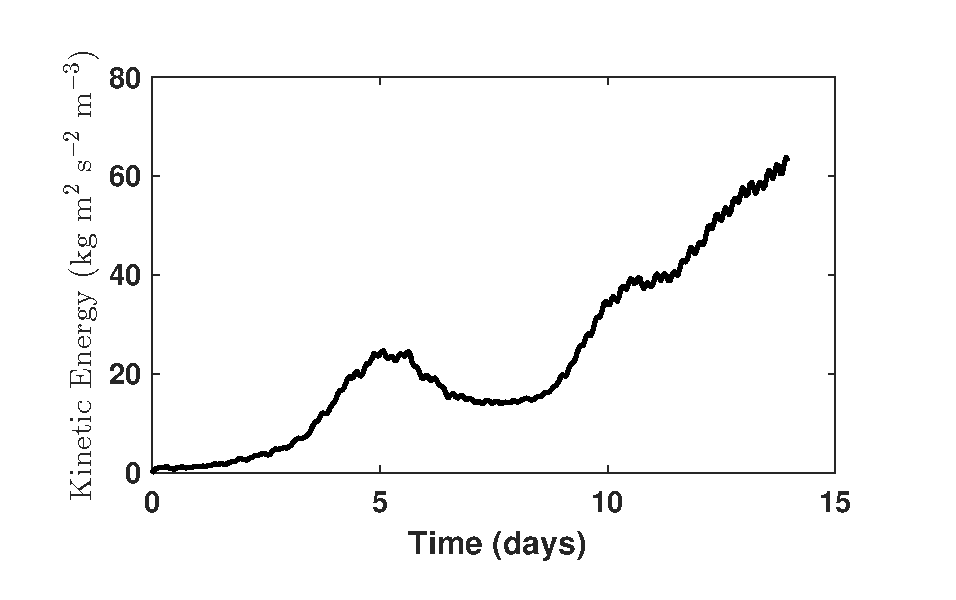
\includegraphics[scale=1]{Chapter3/img/tke}
\caption{Pertubation kinetic energy throughout the simulation. There is a slight drop in the energy between days 6 and 9. The energy again starts to grow around day 12 as the two jets begin to interact as seen in Figure \ref{fig:vortTimeSeries}.}
\label{fig:pke}
\end{figure}

In the next section, the normal mode theory described in Chapter \ref{ch:ch2} is applied to the baroclinic instability simulation presented here. Since we wish to investigate the mesoscale energy spectrum shallowing, results from day 11 are used. We now provide a a closer look at the simulation on day 11.\\

Figure \ref{fig:U_1_Day11} shows the meridional slice of the zonal velocity field at $x = 0$ and $x = L_x/4$, while Figure \ref{fig:U_2_Day11} shows the zonal velocity field at $x = L_x/2$ and $x = 3/4 L_x$. Figure \ref{fig:U_avg_Day11} shows the zonal velocity field averaged in the zonal direction. Figures \ref{fig:vortDivDay11_height_75}, \ref{fig:vortDivDay11_height_50}, and \ref{fig:vortDivDay11_height_25} also show the vertical vorticity and horizontal divergence on day 11 at heights of 250 hPa, 500 hPa, and 750 hPa, respectively. 


\begin{figure}[H]
\vspace{-2em}
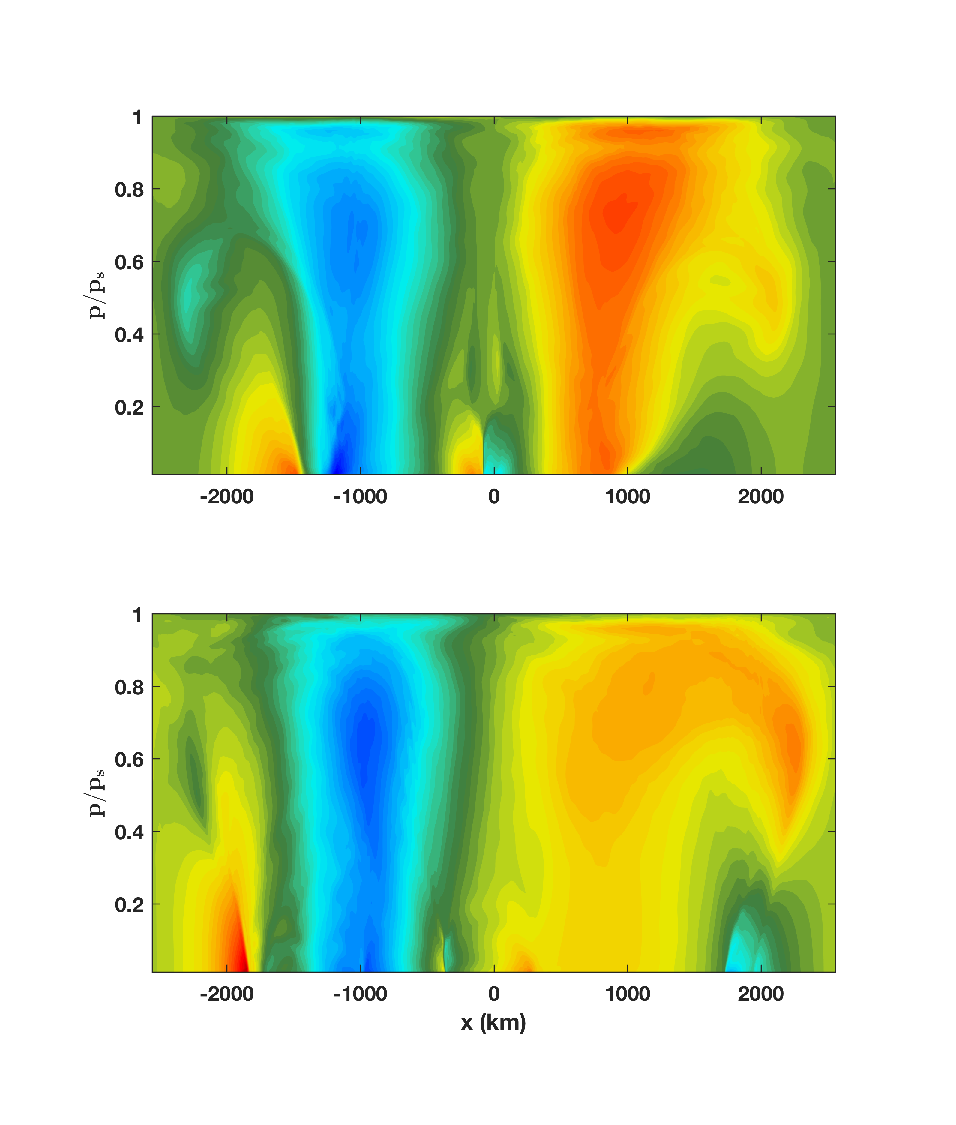
\includegraphics[scale=1]{Chapter3/img/U_1_Day11}
\caption{Zonal velocity field at $x = 0$ (top) and $x = L_x/4$ (bottom).}
\label{fig:U_1_Day11}
\end{figure}

\begin{figure}[H]
\vspace{-2em}
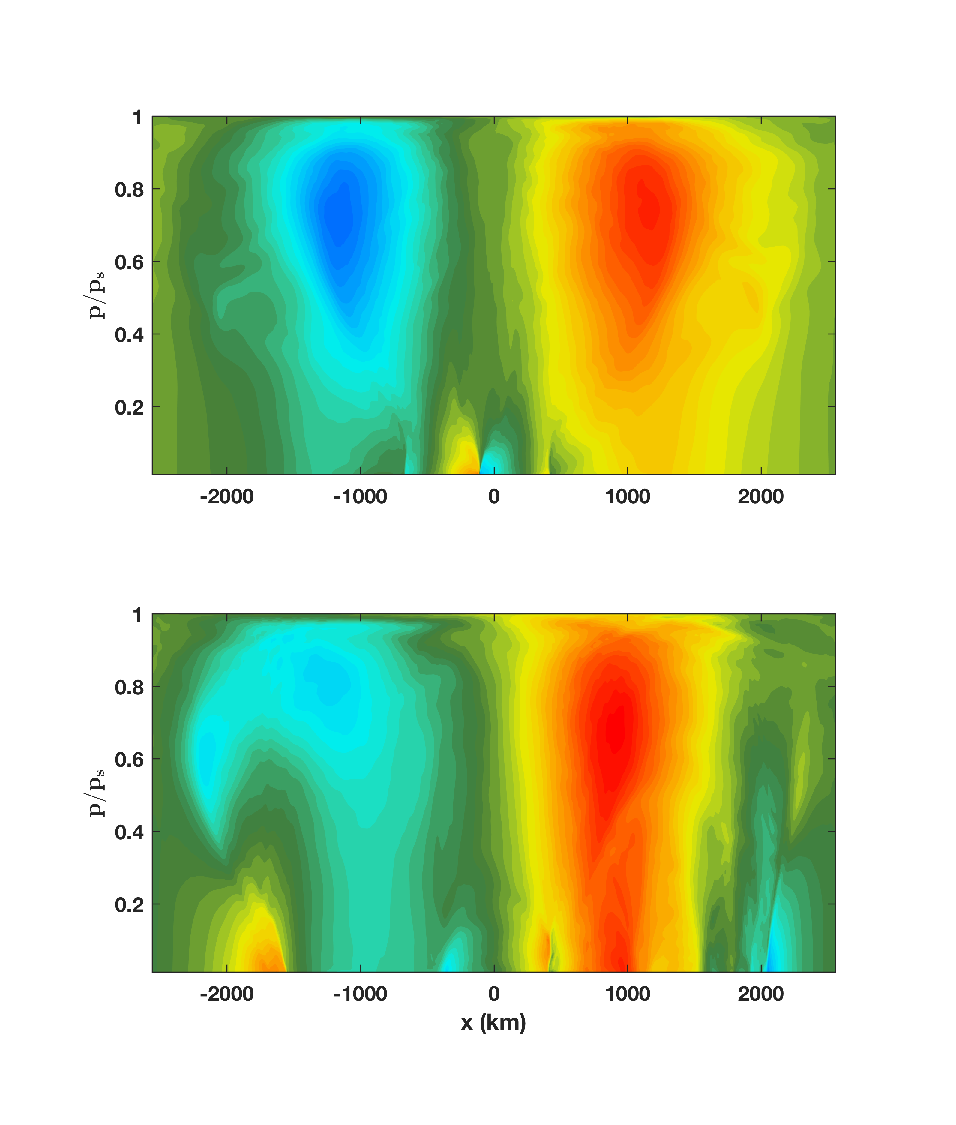
\includegraphics[scale=1]{Chapter3/img/U_2_Day11}
\caption{Zonal velocity field at $x = L_x/2$ (top) and $x = 3/4 L_x$ (bottom).}
\label{fig:U_2_Day11}
\end{figure}

\begin{figure}[H]
\vspace{-2em}
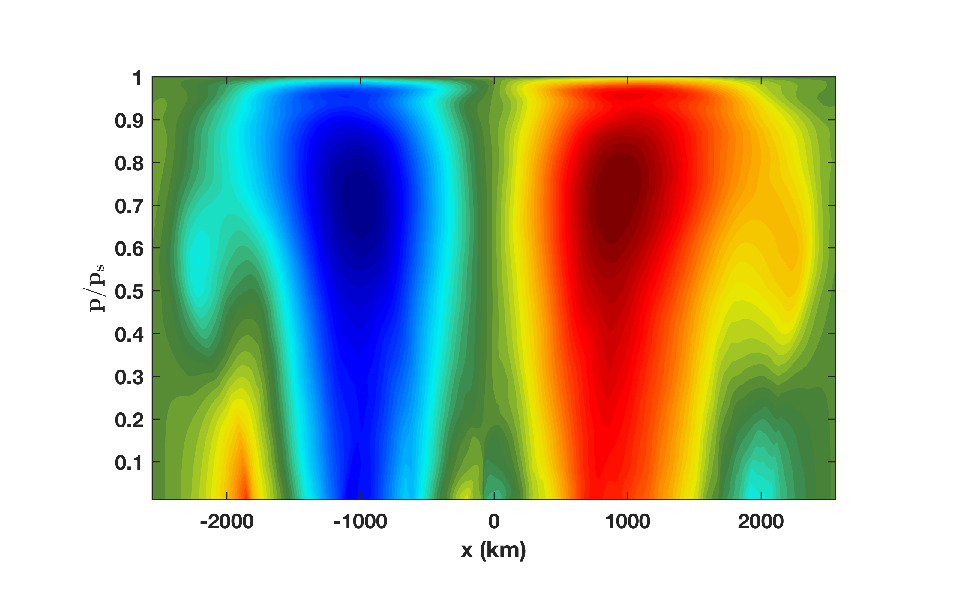
\includegraphics[scale=1]{Chapter3/img/U_avg_Day11}
\caption{Zonal mean of the zonal velocity field}
\label{fig:U_avg_Day11}
\end{figure}

\begin{figure}[H]
\vspace{-2em}
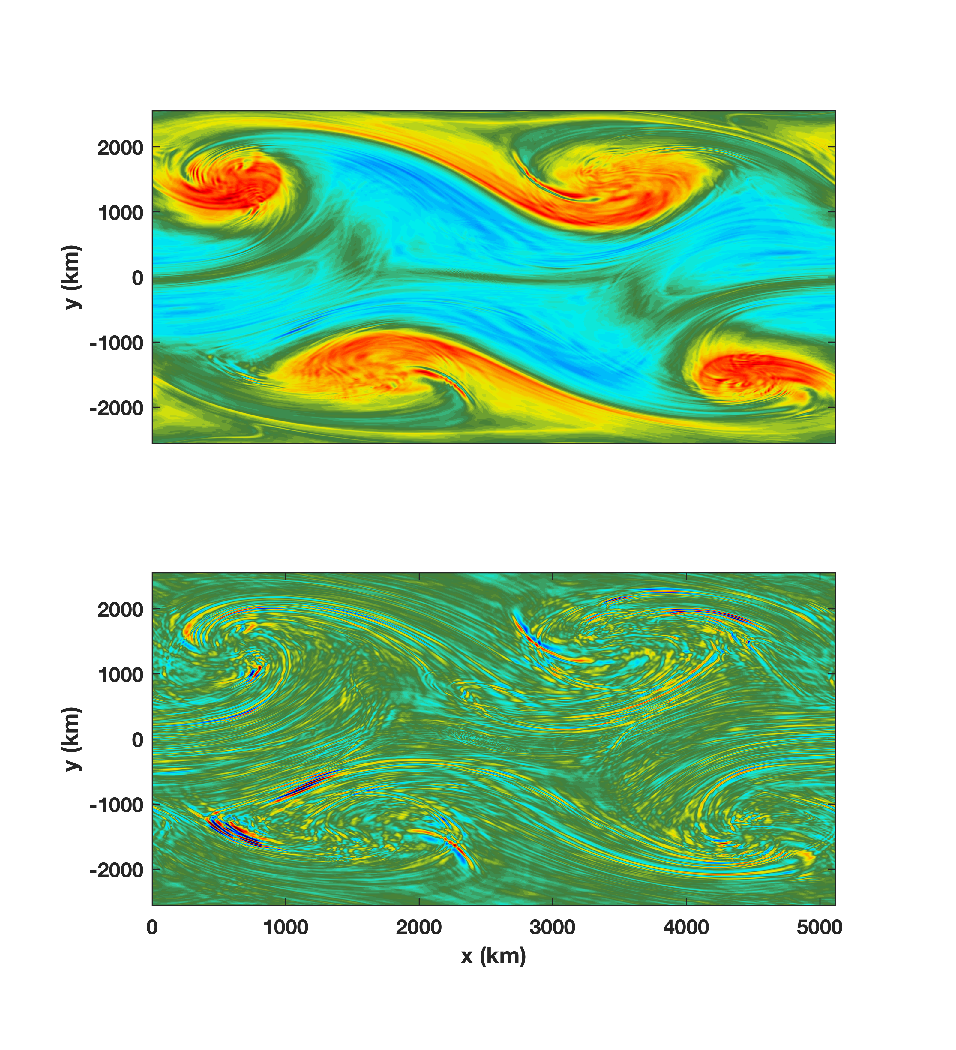
\includegraphics[scale=1]{Chapter3/img/vortDivDay11_height_75}
\caption{Horizontal slices of vertical vorticity (top) and horizontal divergence (bottom) taken during day 11 of the simulation at a height of 250 hPa. The color map has units of $f$, range from $-2f$ to $2f$.}
\label{fig:vortDivDay11_height_75}
\end{figure}

\begin{figure}[H]
\vspace{-2em}
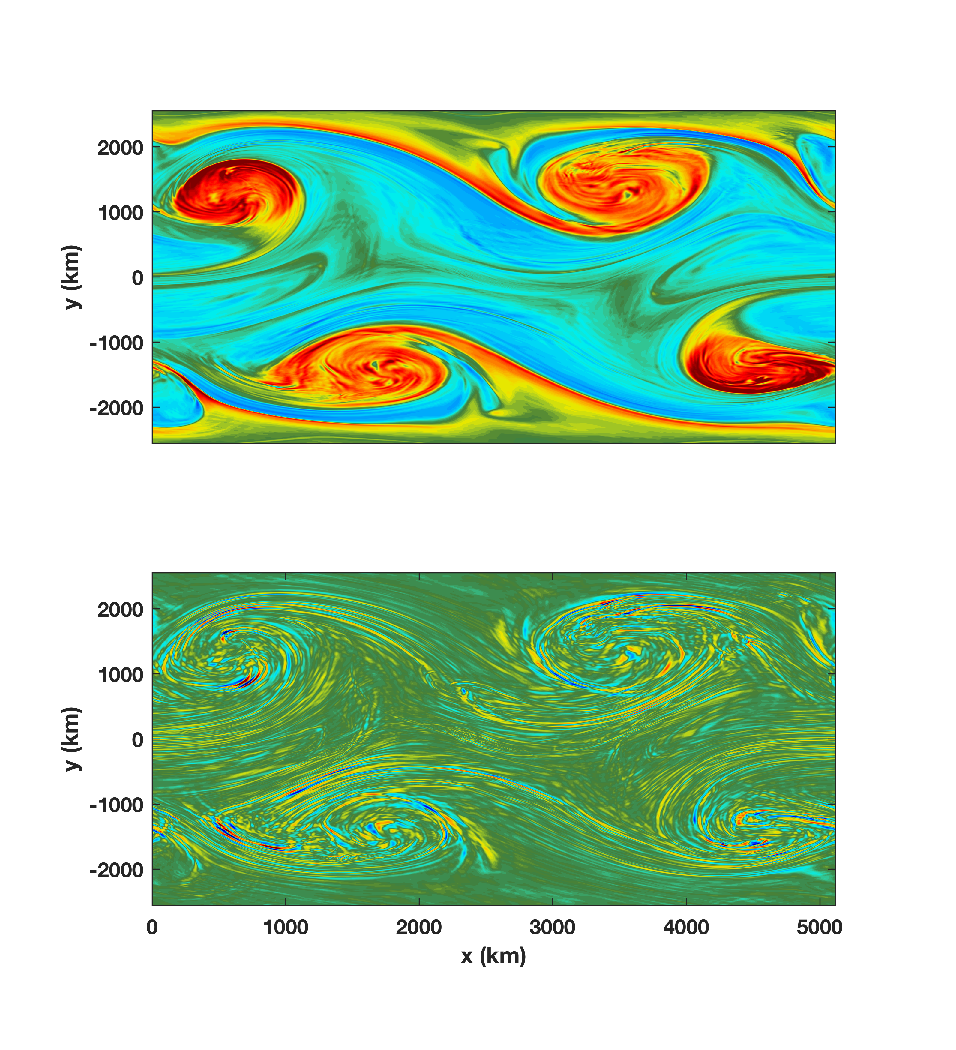
\includegraphics[scale=1]{Chapter3/img/vortDivDay11_height_50}
\caption{As in Figure \ref{fig:vortDivDay11_height_75}, but at a height of 500 hPa.}
\label{fig:vortDivDay11_height_50}
\end{figure}

\begin{figure}[H]
\vspace{-2em}
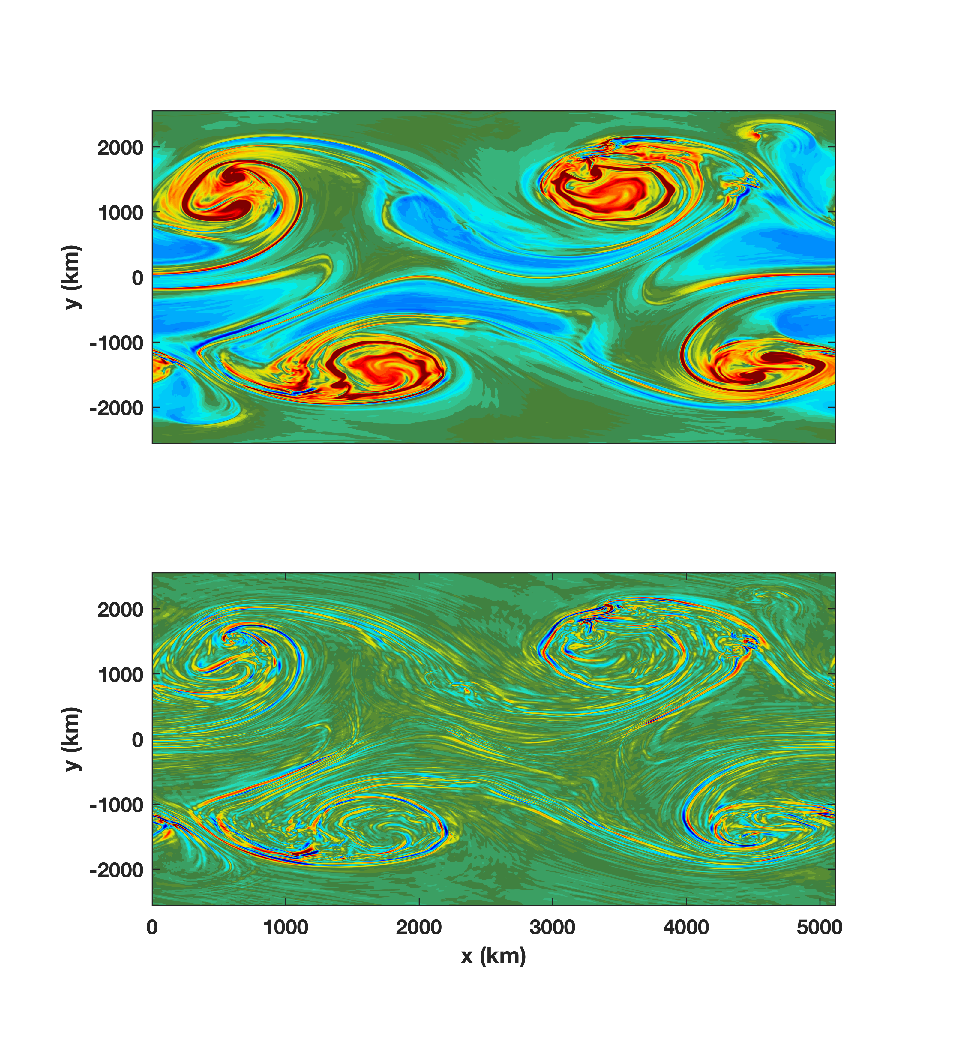
\includegraphics[scale=1]{Chapter3/img/vortDivDay11_height_25}
\caption{As in Figure \ref{fig:vortDivDay11_height_25}, but at a height of 750 hPa.}
\label{fig:vortDivDay11_height_25}
\end{figure}
\chapter{Results}
\label{ch:ch4}
In this chapter, we present the results of the normal mode decomposition compared to the Helmholtz decomposition. In addition to examining the decomposition as a function of vertical mode number, we focus attention on the mesoscale. The discussion and analysis of these results is saved until Chapter \ref{ch:ch5}.

\section{Normal Mode Decomposition}
\subsection{Individual Vertical Modes}
The normal mode decomposition described in Chapter \ref{ch:ch2} is different than the Helmholtz decomposition for a few reasons. The normal mode decomposition splits the total energy (kinetic plus potential) into geostrophic and ageostrophic motion. The normal mode decomposition also provides a way to look at the energy contained in each vertical mode and how the geostrophic and ageostrophic spectra vary as the vertical scale gets smaller.\\

Applying the normal mode decomposition to the jet described in Chapter \ref{ch:ch3} leads to the normal mode structure seen in Figure \ref{fig:normalmodes}, as well as equivalent depths in Table \ref{tab:equivDepths}. Once the normal modes are solved, we project the horizontal velocity and geopotential fields to each mode. First, we show the barotropic mode in Figure \ref{fig:barotropicKEPE}, which corresponds to vertical mode 0. The largest scales corresponding to the smallest non-dimensional wavenumbers, $\tilde{k} = L_x/2\pi |\mathbf{k}|$, represent wavelengths of around 5000 km, while the largest values of $\tilde{k}$ represent wavelengths as small as 10 km. The mesoscale is shown around $\tilde{k} \approx 6$ to 60. Near the larger wavenumbers, at  $\tilde{k} \approx 300$, the spectra quickly steepen as the energy contained at these scales goes to zero. This is due to the numerical dissipation inherent in the WRF discretization. Finally, since the energy is binned over circles of constant radius in the $k-l$ plane according to equation (\ref{eq:binning}), all of the energy that is outside the circle of radius $\tilde{k}_{\text{max}} = 512$ is binned together at the end.\\

The barotropic mode is qualitatively a little different from the baroclinic modes. Perhaps the most notable difference of the barotropic mode is the difference between the DKE and ageostrophic spectra. The DKE of the barotropic mode is very different from the ageostrophic mode, where the ageostrophic spectrum stays roughly constant at a -4.0 slope across all length scales, while  DKE spectrum rapidly shallows from a -3.7 slope in the synoptic scale to a -2.6 slope in the mesoscale. The vertical structure of the barotropic mode is nearly constant, which corresponds to the largest equivalent depth.  \\

Each vertical mode from the normal mode decomposition employed in this thesis is a boundary value problem that covers the full extent of the atmosphere. For this reason, to best make a comparison to the Helmholtz decomposition, we average the 2D horizontal RKE and DKE spectra over the entire depth of the atmosphere. This is different from most of the literature (e.g. \cite{Hamilton2008}, \cite{Skamarock2008a}, \cite{Waite2009}, \cite{Peng2013}, \cite{Waite2013}), which averages over different regions of the atmosphere (e.g. upper troposphere, tropopause, stratosphere), or consider specific vertical levels, due in part to the different stratification profiles. 

\begin{figure}[H]
\vspace{-3cm}
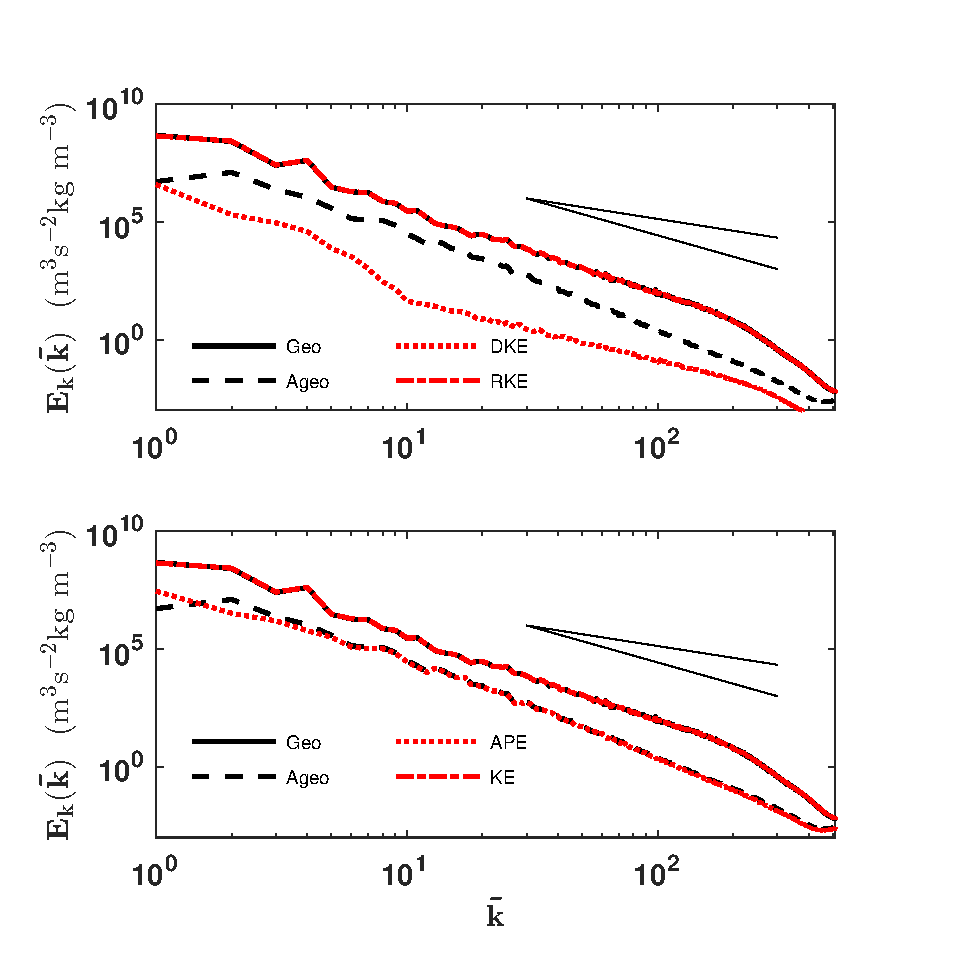
\includegraphics[scale=1]{Chapter4/img/GeoAgeoBarotropic}
\vspace{-1cm}
\caption{Energy spectra of barotropic mode. The top shows the geostrophic (black solid) and ageostrophic (black dashed) modes along with the rotational (red dash-dot) and the divergent (red dotted) kinetic energy spectra. The bottom shows the geostrophic (black solid) and ageostrophic (black dashed) modes versus the kinetic energy (red dash-dot) and potential energy (red dotted). Reference lines with $-5/3$ and $-3$ slopes are shown in the upper right.}
\label{fig:barotropicKEPE}
\end{figure}

The baroclinic modes correspond to normal modes with changing vertical structure. As the mode number increases, the equivalent depth of the associated shallow water system decreases as well as the number of zero crossings, which corresponds to a length scale that can be thought of as a ``wavelength'' of the vertical mode. Figures \ref{fig:GeoAgeo_RKEDKE_1-3} - \ref{fig:GeoAgeo_RKEDKE_29} show the energy spectra of the first 30 baroclinic modes. For conciseness, only the odd numbered vertical modes are shown.\\

In the baroclinic modes, it is immediately apparent that there is closer agreement between the DKE spectrum and the ageostrophic spectrum slopes. For the first several vertical modes, the rotational kinetic energy spectrum and the geostrophic energy spectrum agree well at all but the largest of scales. It is also evident that with increasing vertical mode number, the RKE and DKE spectra begin to shallow at a much more pronounced rate than the geostrophic and ageostrophic spectra (see Figure \ref{fig:slopes}). Another observation from the baroclinic spectra show that as the vertical mode number increases, the energy in the mesoscale increases in the geostrophic and DKE spectra. \\

\begin{figure}[H]
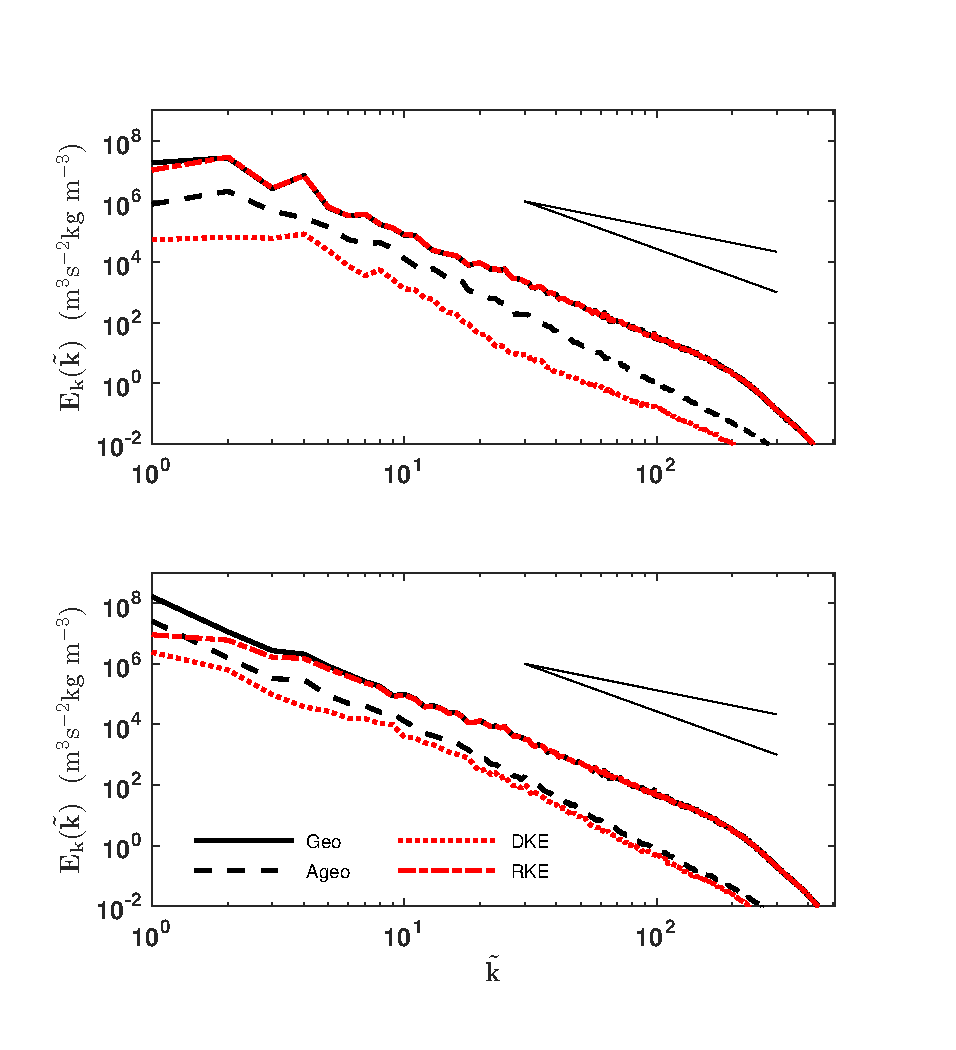
\includegraphics[scale=1]{Chapter4/img/GeoAgeo_RKEDKE_1-3}
\vspace{-3em}
\caption{Vertical modes 1 (top) and 3 (bottom). Both figures show the geostrophic (black solid) and ageostrophic (black dashed) modes compared to the RKE (red dash dot) and DKE (red dotted). $-5/3$ and $-3$ references are shown in the upper right. The wavenumber corresponding to $f/c_n$ is $\tilde{k} = 0.65$ for mode 1 and $\tilde{k} = 1.5$ for mode 3.}
\label{fig:GeoAgeo_RKEDKE_1-3}
\end{figure}

\begin{figure}[H]
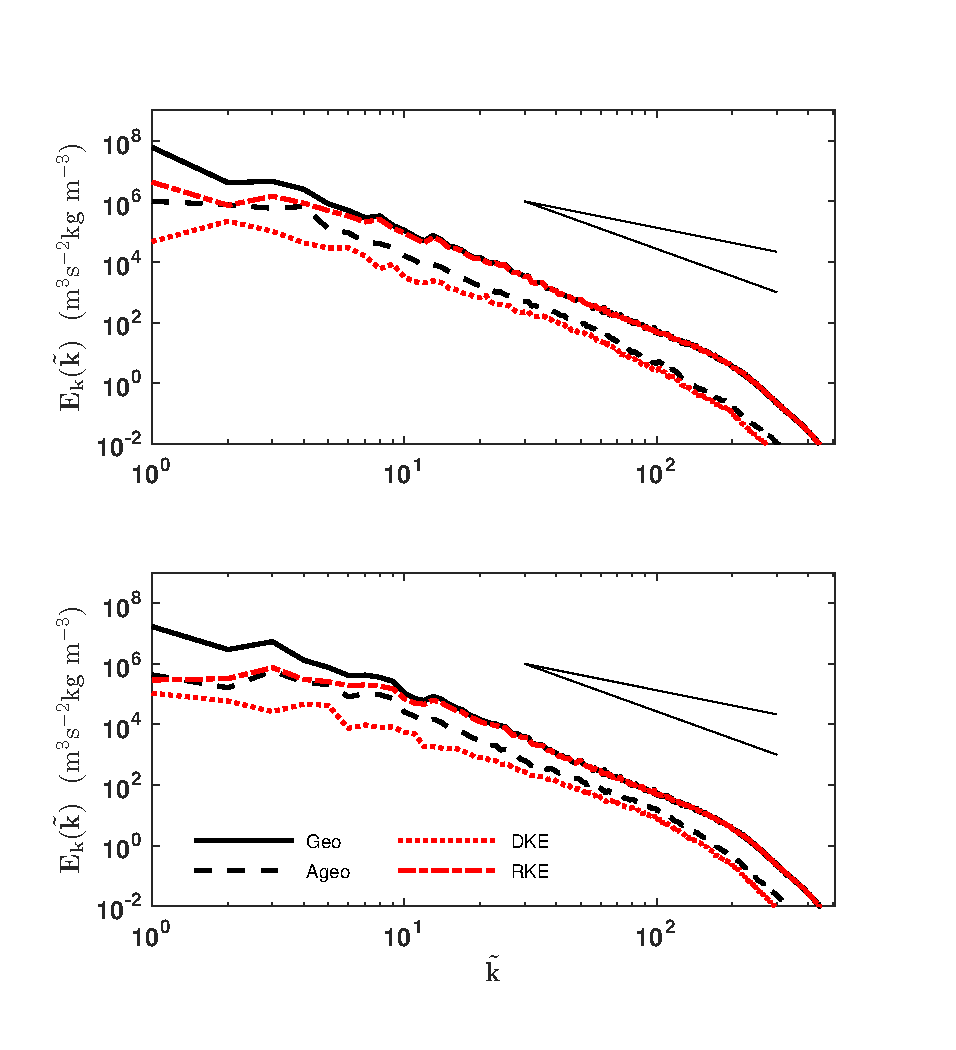
\includegraphics[scale=1]{Chapter4/img/GeoAgeo_RKEDKE_5-7}
\caption{The same as in Figure \ref{fig:GeoAgeo_RKEDKE_1-3}, but for vertical modes 5 (top) and 7 (bottom).  The wavenumber corresponding to $f/c_n$ is  $\tilde{k} = 2.5$ for mode 5 and $\tilde{k} = 3.6$ for mode 7.}
\label{fig:GeoAgeo_RKEDKE_5-7}
\end{figure}

\begin{figure}[H]
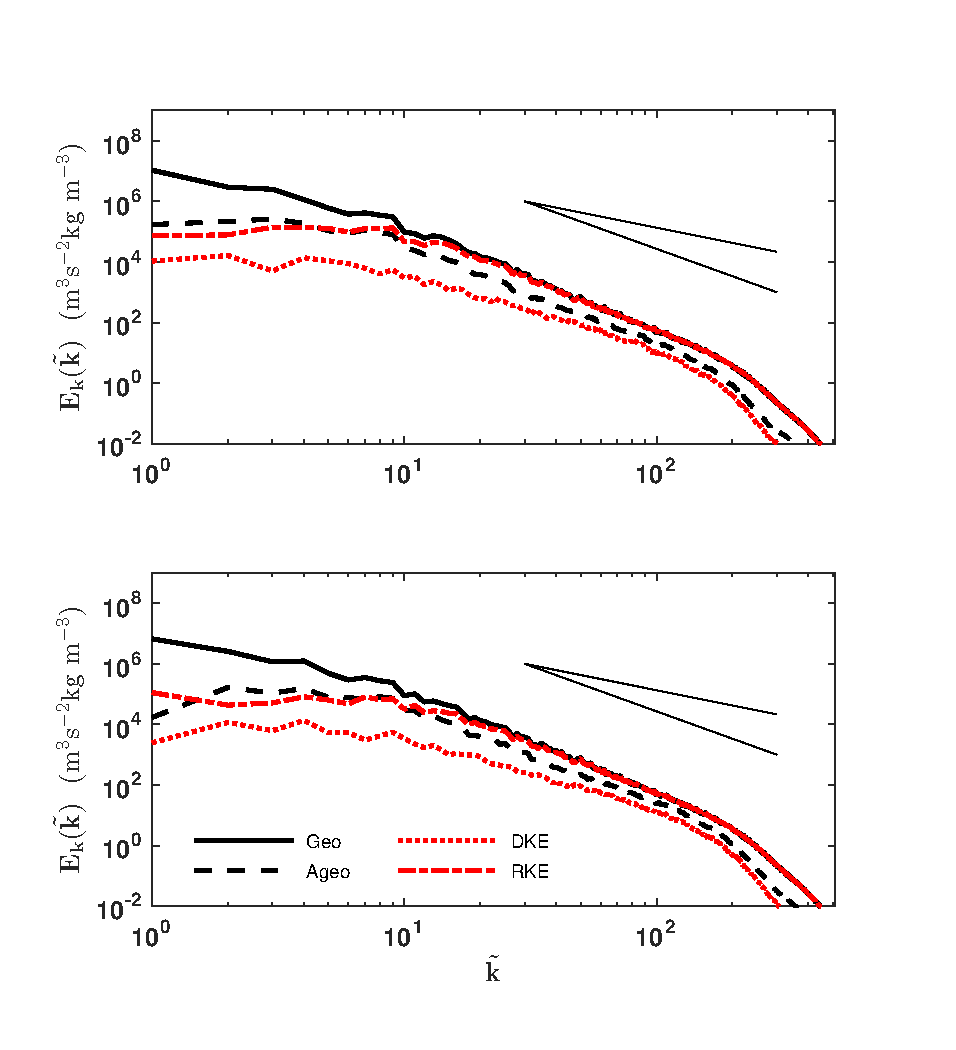
\includegraphics[scale=1]{Chapter4/img/GeoAgeo_RKEDKE_9-11}
\caption{The same as in Figure \ref{fig:GeoAgeo_RKEDKE_1-3}, but for vertical modes 9 (top) and 11 (bottom).  The wavenumber corresponding to $f/c_n$ is $\tilde{k} = 4.9$ for mode 9 and $\tilde{k} = 6.1$ for mode 11.}
\label{fig:GeoAgeo_RKEDKE_9-11}
\end{figure}

\begin{figure}[H]
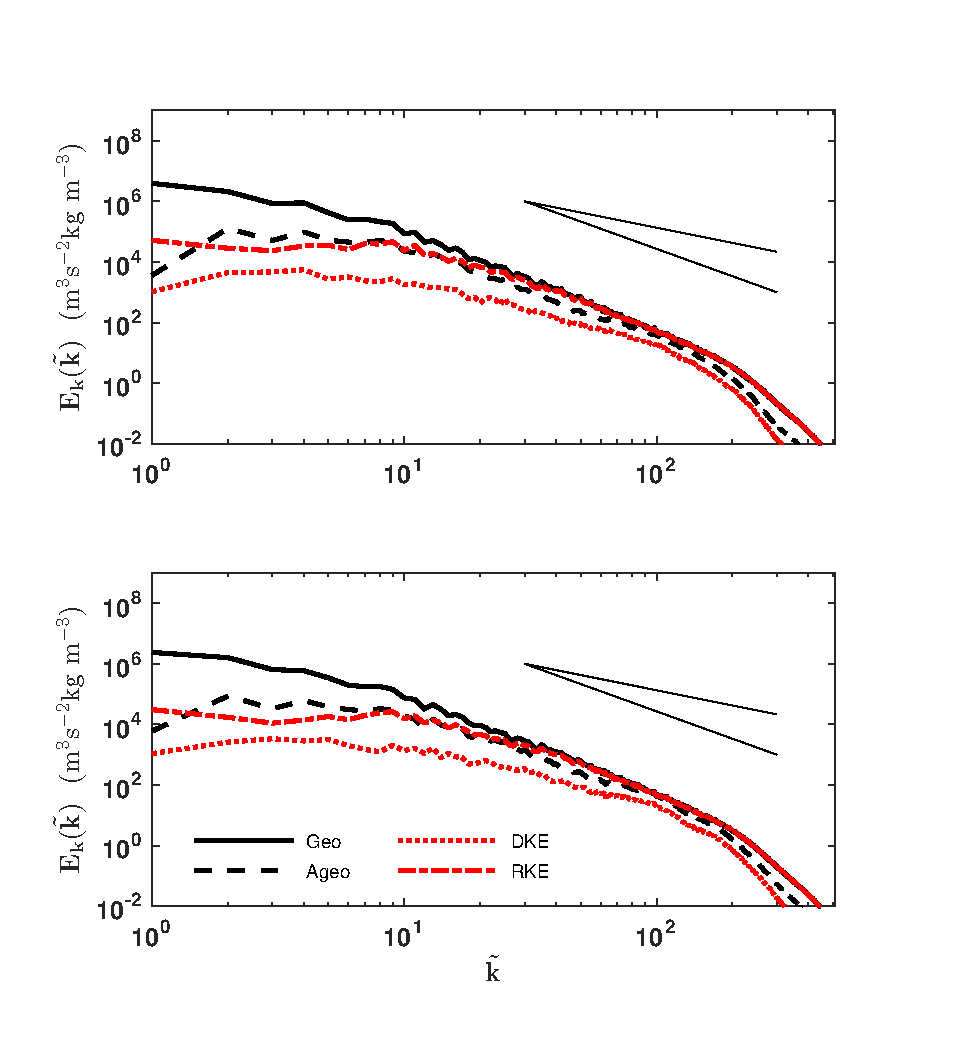
\includegraphics[scale=1]{Chapter4/img/GeoAgeo_RKEDKE_13-15}
\caption{The same as in Figure \ref{fig:GeoAgeo_RKEDKE_1-3}, but for vertical modes 13 (top) and 15 (bottom).  The wavenumber corresponding to $f/c_n$ is $\tilde{k} = 7.5$ for mode 13 and $\tilde{k} = 8.9$ for mode 15.}
\label{fig:GeoAgeo_RKEDKE_13-15}
\end{figure}

\begin{figure}[H]
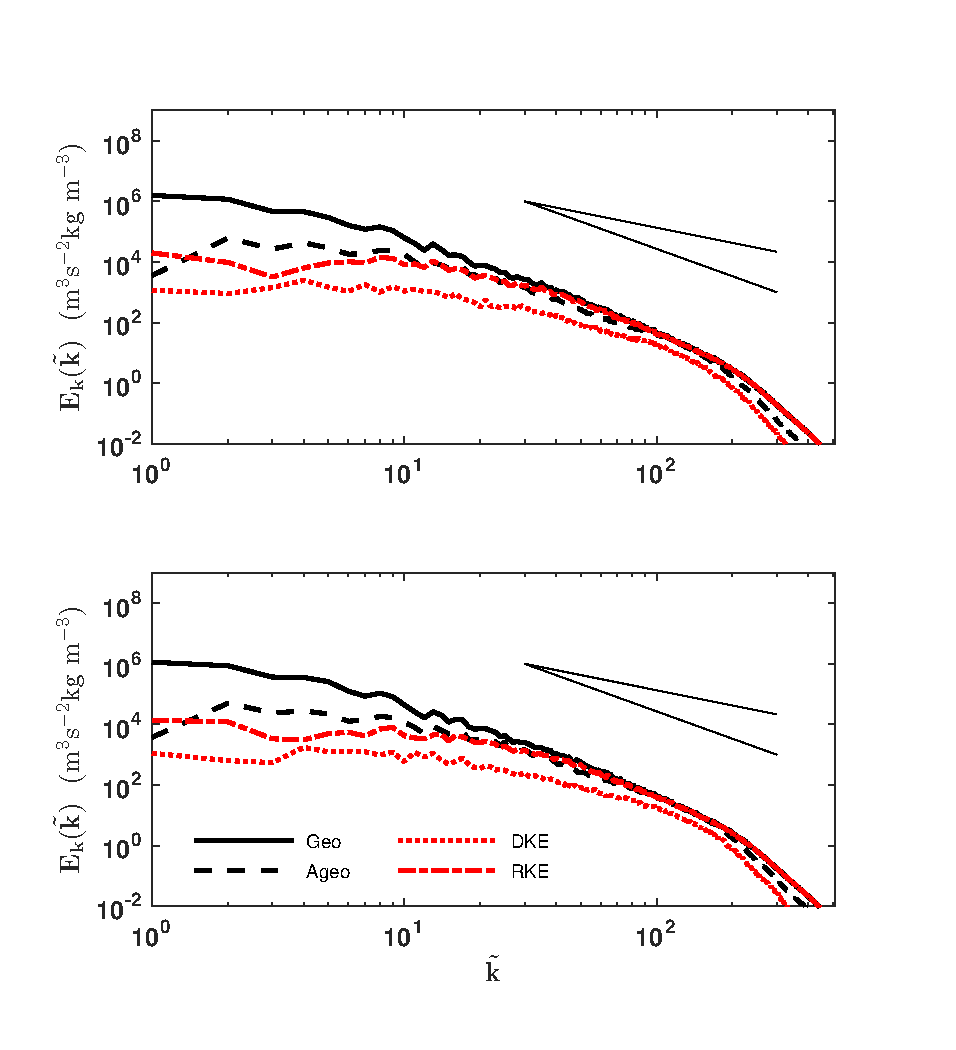
\includegraphics[scale=1]{Chapter4/img/GeoAgeo_RKEDKE_17-19}
\caption{The same as in Figure \ref{fig:GeoAgeo_RKEDKE_1-3}, but for vertical modes 17 (top) and 19 (bottom).  The wavenumber corresponding to $f/c_n$ is $\tilde{k} = 10.3$ for mode 17 and $\tilde{k} = 11.8$ for mode 19.}
\label{fig:GeoAgeo_RKEDKE_17-19}
\end{figure}

\begin{figure}[H]
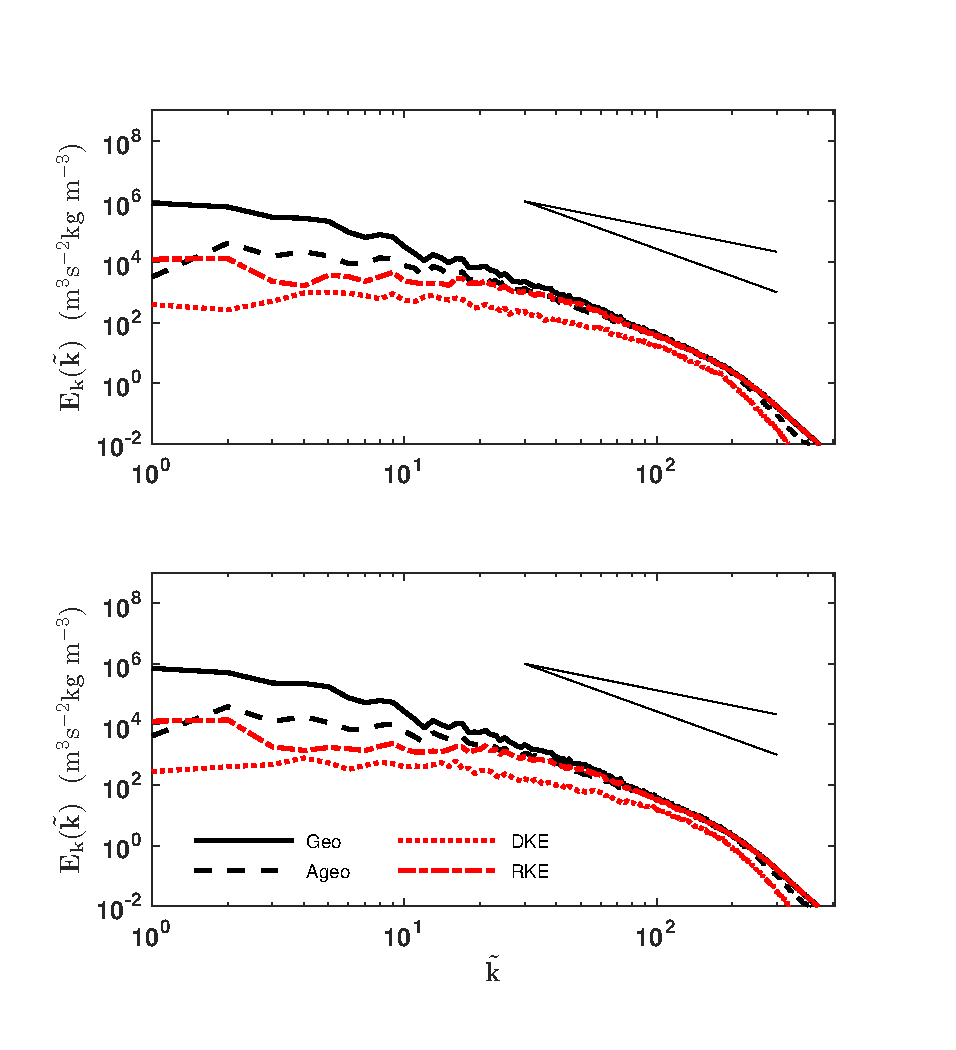
\includegraphics[scale=1]{Chapter4/img/GeoAgeo_RKEDKE_21-23}
\caption{The same as in Figure \ref{fig:GeoAgeo_RKEDKE_1-3}, but for vertical modes 21 (top) and 23 (bottom).  The wavenumber corresponding to $f/c_n$ is $\tilde{k} = 13.4$ for mode 21 and $\tilde{k} = 15$ for mode 23.}
\label{fig:GeoAgeo_RKEDKE_21-23}
\end{figure}

\begin{figure}[H]
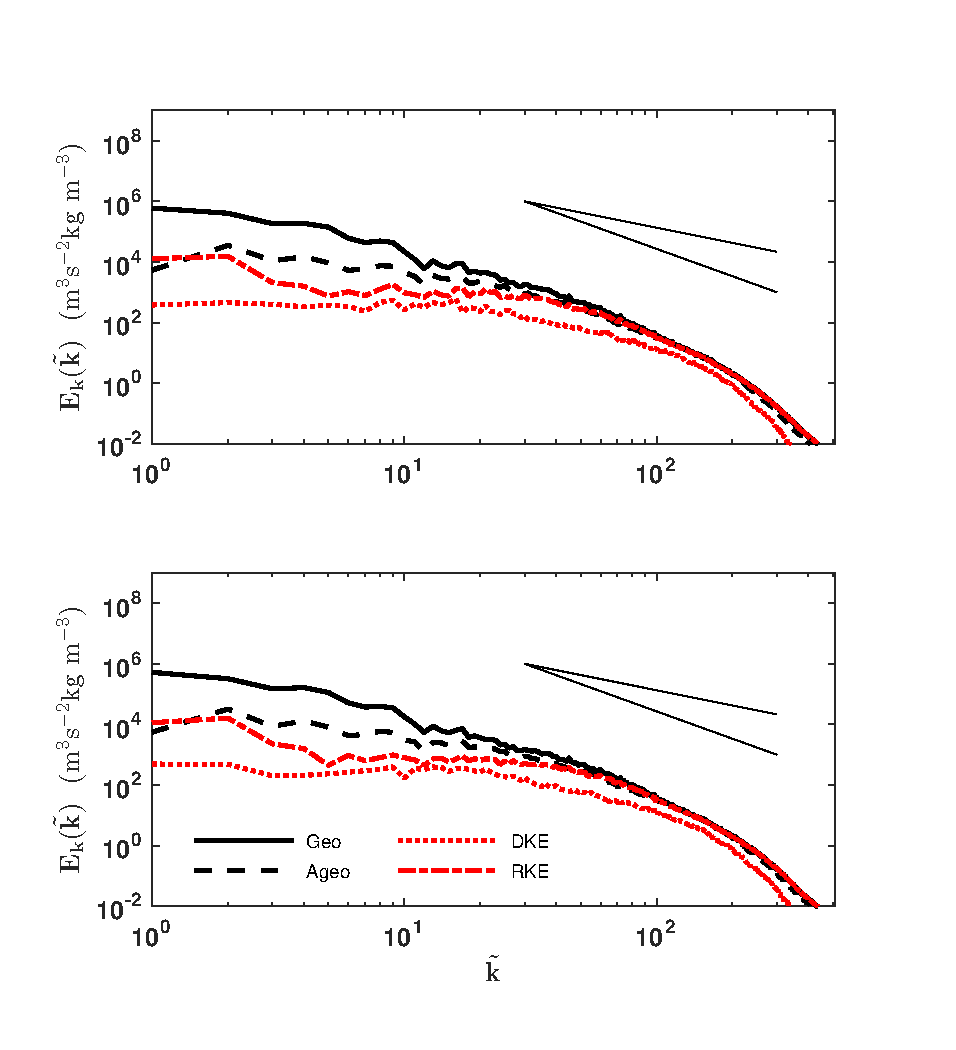
\includegraphics[scale=1]{Chapter4/img/GeoAgeo_RKEDKE_25-27}
\caption{The same as in Figure \ref{fig:GeoAgeo_RKEDKE_1-3}, but for vertical modes 25 (top) and 27 (bottom).  The wavenumber corresponding to $f/c_n$ is $\tilde{k} = 16.6$ for mode 25 and $\tilde{k} = 18.3$ for mode 27.}
\label{fig:GeoAgeo_RKEDKE_25-27}
\end{figure}

\begin{figure}[H]
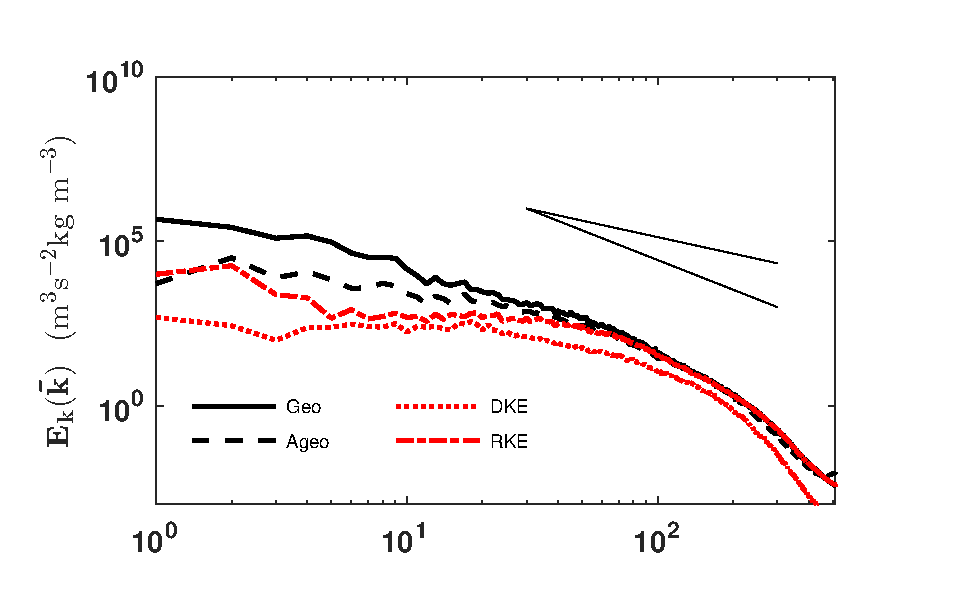
\includegraphics[scale=1]{Chapter4/img/GeoAgeo_RKEDKE_29}
\caption{The same as in Figure \ref{fig:GeoAgeo_RKEDKE_1-3}, but for vertical mode 29.  The wavenumber corresponding to $f/c_n$ for this mode is $\tilde{k} = 20.1$.}
\label{fig:GeoAgeo_RKEDKE_29}
\end{figure}

\subsection{Examining the Composition of the Normal Modes}
It is also useful to compare to include the potential energy alongside the RKE and DKE  to further understand the role each of these quantities have in establishing the geostrophic and ageostrophic spectra. Figures \ref{fig:Geo_APERKE_1-3} - \ref{fig:Geo_APERKE_29} show the geostrophic modes along with the RKE and available potential energy (APE) per vertical mode. Since the geostrophic mode is non-divergent, the DKE is omitted for clarity. Unlike the geostrophic modes, the ageostrophic modes have non-zero divergence. Figures \ref{fig:Ageo_APEDKE_1-3} - \ref{fig:Ageo_APEDKE_29} show the ageostrophic modes with the DKE, RKE, and APE per vertical mode.

%%%%%%%%%%%%
\begin{figure}[H]
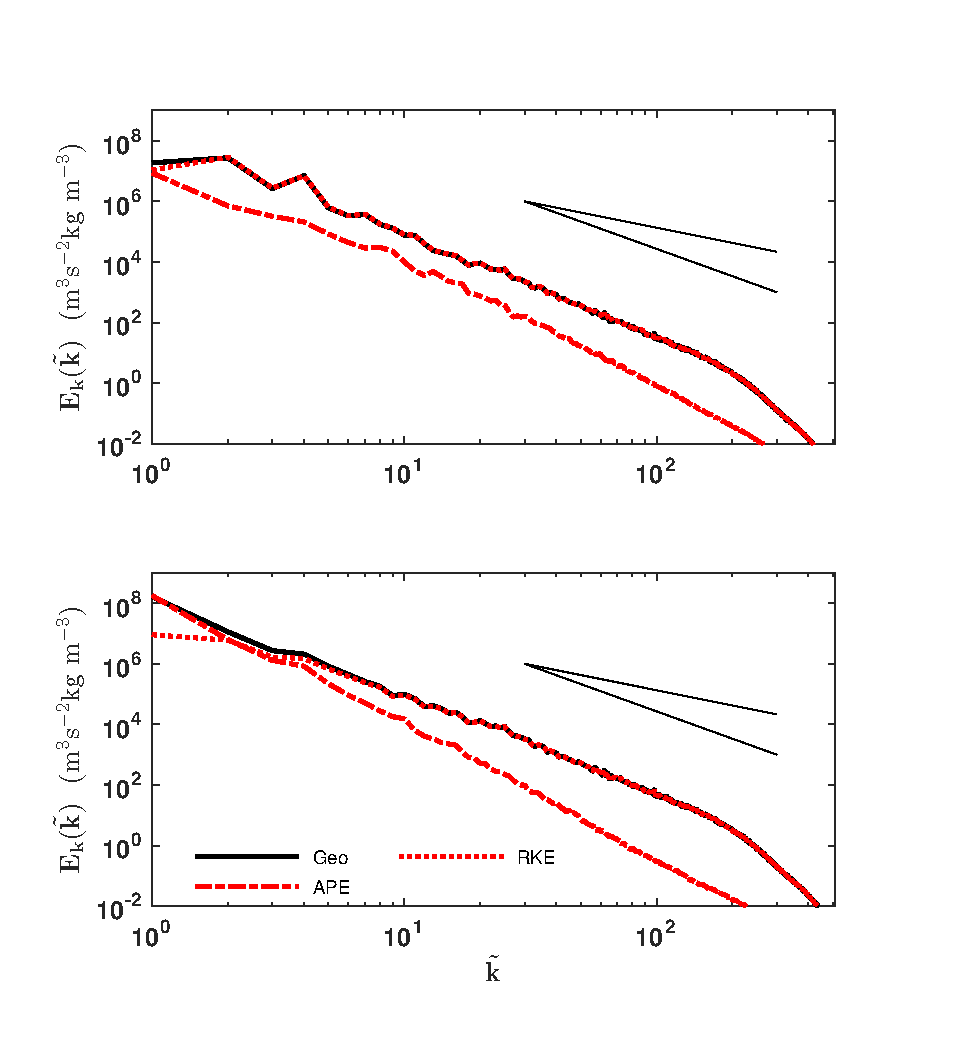
\includegraphics[scale=1]{Chapter4/img/Geo_APERKE_1-3}
\caption{Geostrophic (black solid), APE (red dash-dot), and RKE (red dotted) spectra for vertical modes 1 (top) and 3 (bottom). The geostrophic mode is mostly overlapped by the RKE. The wavenumber corresponding to $f/c_n$ for this mode is $\tilde{k} = 0.65$ for mode 1 and $\tilde{k} = 1.5$ for mode 3.}
\label{fig:Geo_APERKE_1-3}
\end{figure}

\begin{figure}[H]
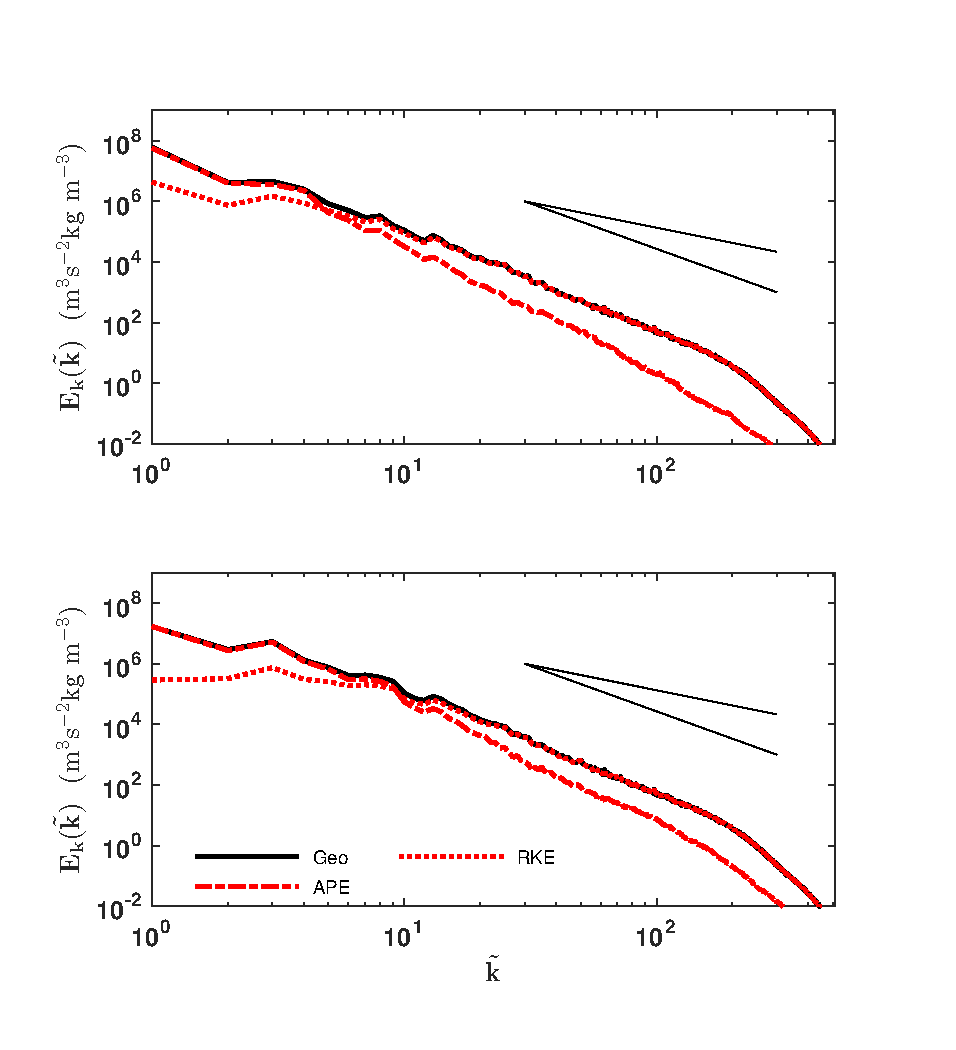
\includegraphics[scale=1]{Chapter4/img/Geo_APERKE_5-7}
\caption{The same as in Figure \ref{fig:Geo_APERKE_1-3}, but for vertical modes 5 (top) and 7 (bottom). The geostrophic mode is mostly overlapped by the RKE. The wavenumber corresponding to $f/c_n$ is $\tilde{k} = 2.5$ for mode 5 and $\tilde{k} = 3.6$ for mode 7.}
\label{fig:Geo_APERKE_5-7}
\end{figure}

\begin{figure}[H]
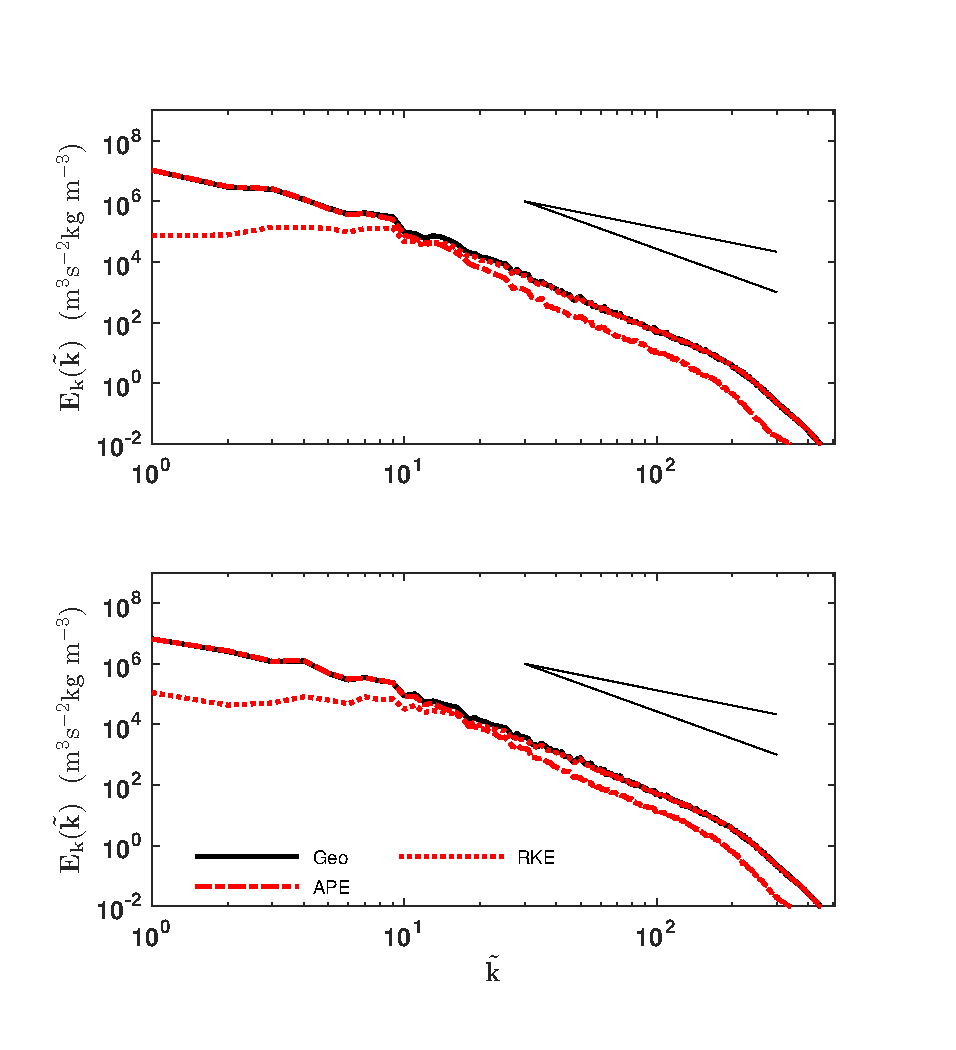
\includegraphics[scale=1]{Chapter4/img/Geo_APERKE_9-11}
\caption{The same as in Figure \ref{fig:Geo_APERKE_1-3}, but for vertical modes 9 (top) and 11 (bottom). The geostrophic mode is mostly overlapped by the APE and RKE. The wavenumber corresponding to $f/c_n$ is $\tilde{k} = 4.9$ for mode 9 and $\tilde{k} = 6.1$ for mode 11.}
\label{fig:Geo_APERKE_9-11}
\end{figure}

\begin{figure}[H]
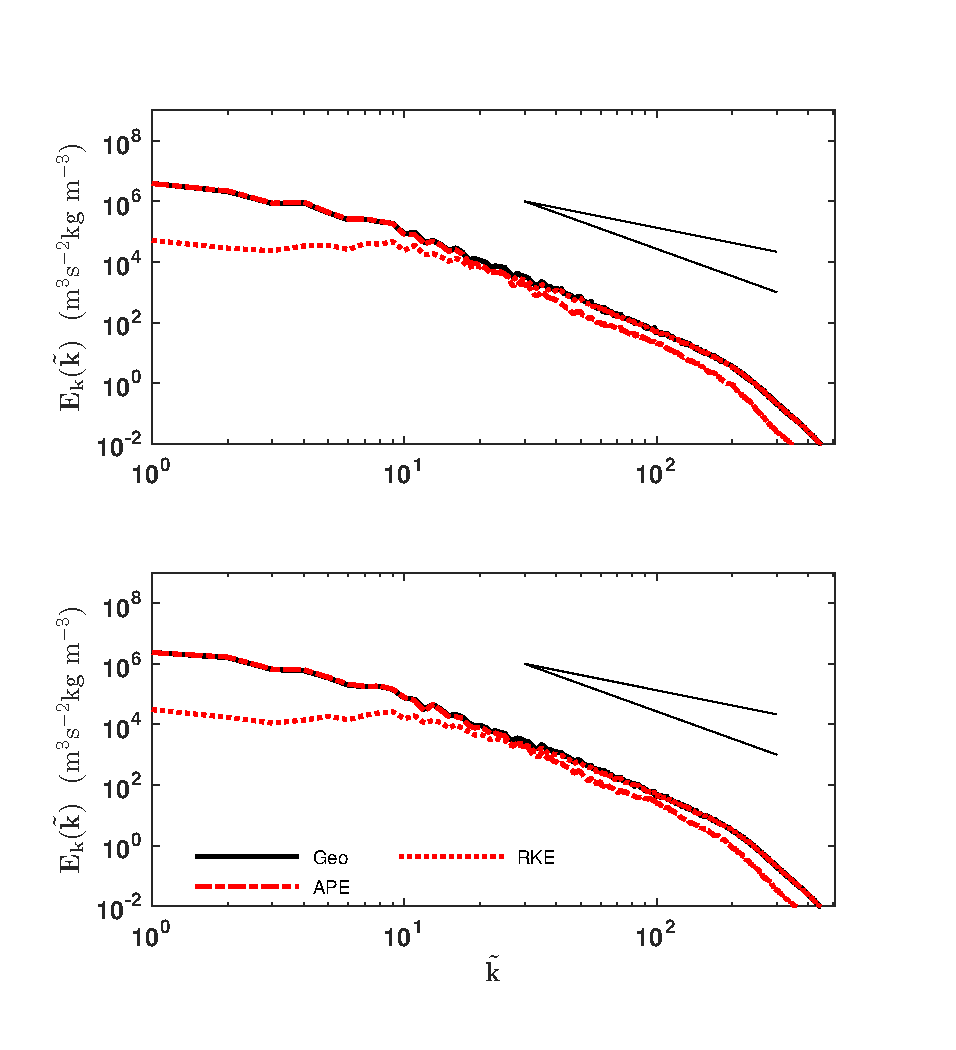
\includegraphics[scale=1]{Chapter4/img/Geo_APERKE_13-15}
\caption{The same as in Figure \ref{fig:Geo_APERKE_1-3}, but for vertical modes 13 (top) and 15 (bottom). The geostrophic mode is mostly overlapped by the APE and RKE. The wavenumber corresponding to $f/c_n$ is $\tilde{k} = 7.5$ for mode 13 and $\tilde{k} = 8.9$ for mode 15.}
\label{fig:Geo_APERKE_13-15}
\end{figure}

\begin{figure}[H]
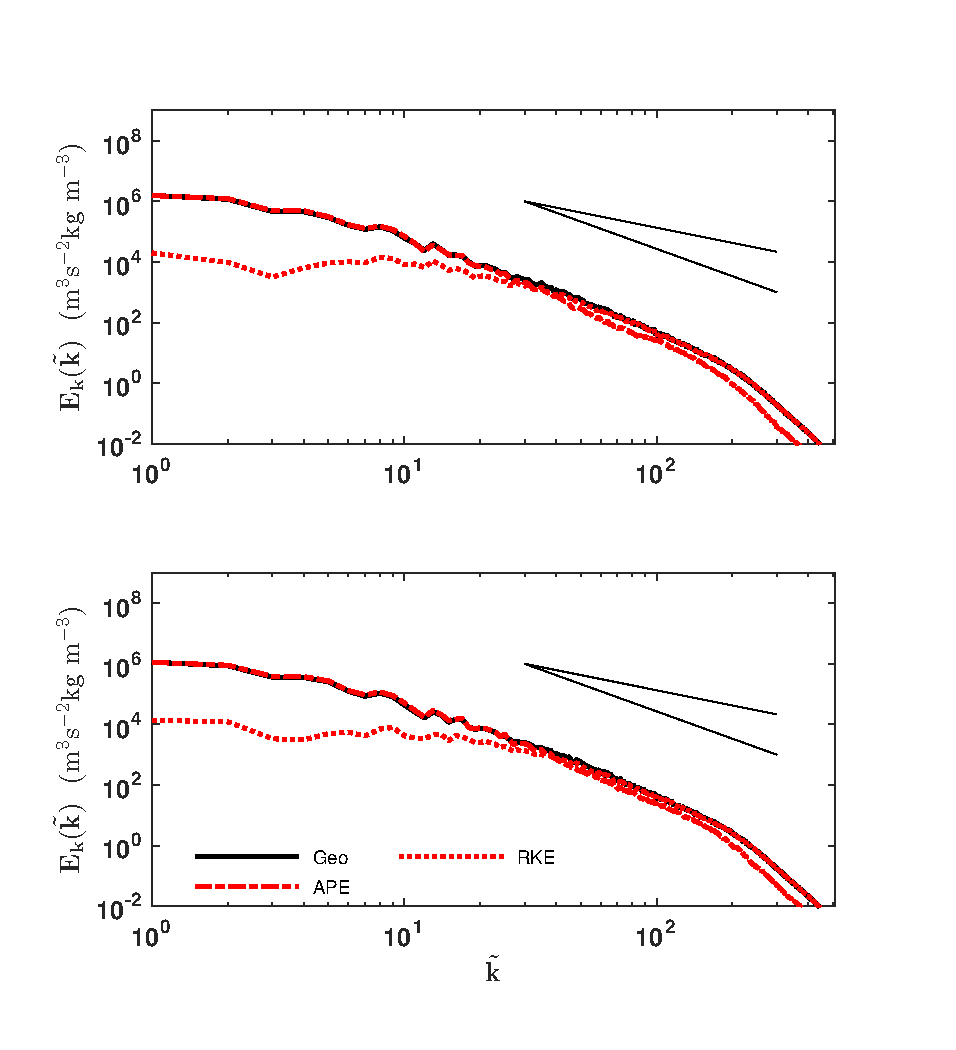
\includegraphics[scale=1]{Chapter4/img/Geo_APERKE_17-19}
\caption{The same as in Figure \ref{fig:Geo_APERKE_1-3}, but for vertical modes 17 (top) and 19 (bottom). The geostrophic mode is mostly overlapped by the APE and RKE. The wavenumber corresponding to $f/c_n$ is $\tilde{k} = 10.3$ for mode 17 and $\tilde{k} = 11.8$ for mode 19.}
\label{fig:Geo_APERKE_17-19}
\end{figure}

\begin{figure}[H]
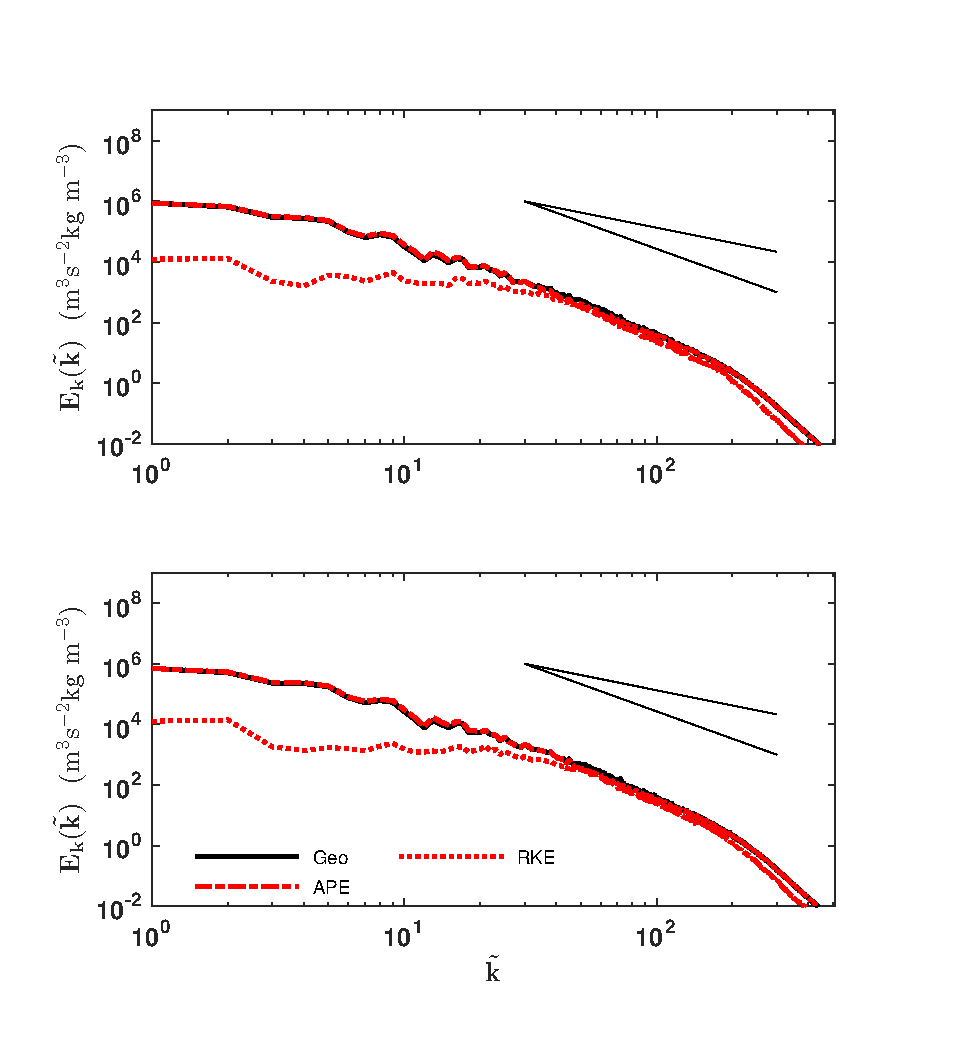
\includegraphics[scale=1]{Chapter4/img/Geo_APERKE_21-23}
\caption{The same as in Figure \ref{fig:Geo_APERKE_1-3}, but for vertical modes 21 (top) and 23 (bottom). The geostrophic mode is mostly overlapped by the APE and RKE. The wavenumber corresponding to $f/c_n$ is $\tilde{k} = 13.4$ for mode 21 and $\tilde{k} = 15$ for mode 23.}
\label{fig:Geo_APERKE_21-23}
\end{figure}

\begin{figure}[H]
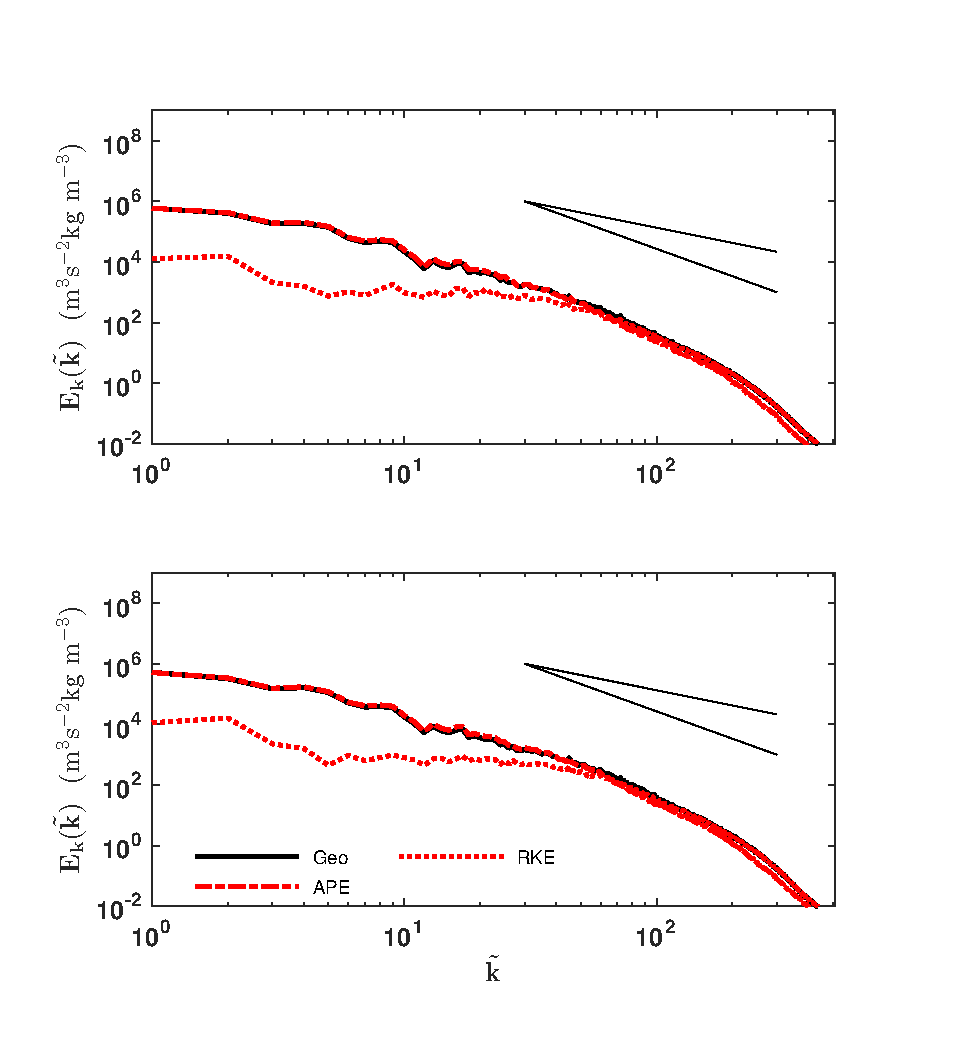
\includegraphics[scale=1]{Chapter4/img/Geo_APERKE_25-27}
\caption{The same as in Figure \ref{fig:Geo_APERKE_1-3}, but for vertical modes 25 (top) and 27 (bottom). The geostrophic mode is mostly overlapped by the APE and RKE. The wavenumber corresponding to $f/c_n$ is $\tilde{k} = 16.6$ for mode 25 and $\tilde{k} = 18.3$ for mode 27.}
\label{fig:Geo_APERKE_25-27}
\end{figure}

\begin{figure}[H]
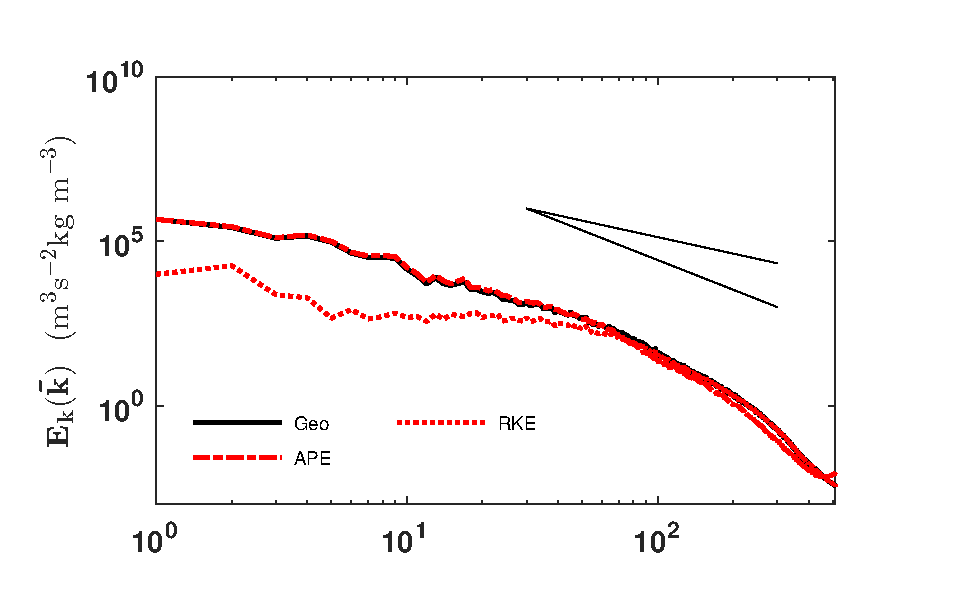
\includegraphics[scale=1]{Chapter4/img/Geo_APERKE_29}
\caption{The same as in Figure \ref{fig:Geo_APERKE_1-3}, but for vertical mode 29. The geostrophic mode is mostly overlapped by the APE and RKE.  The wavenumber corresponding to $f/c_n$ is $\tilde{k} = 20.1$.}
\label{fig:Geo_APERKE_29}
\end{figure}
%%%%%%%%%%%%%%%%%%%%%%%%%%%%%%%%%%%%%%%%%%%%%%%%%%%%%%%%%%%%%%%
\begin{figure}[H]
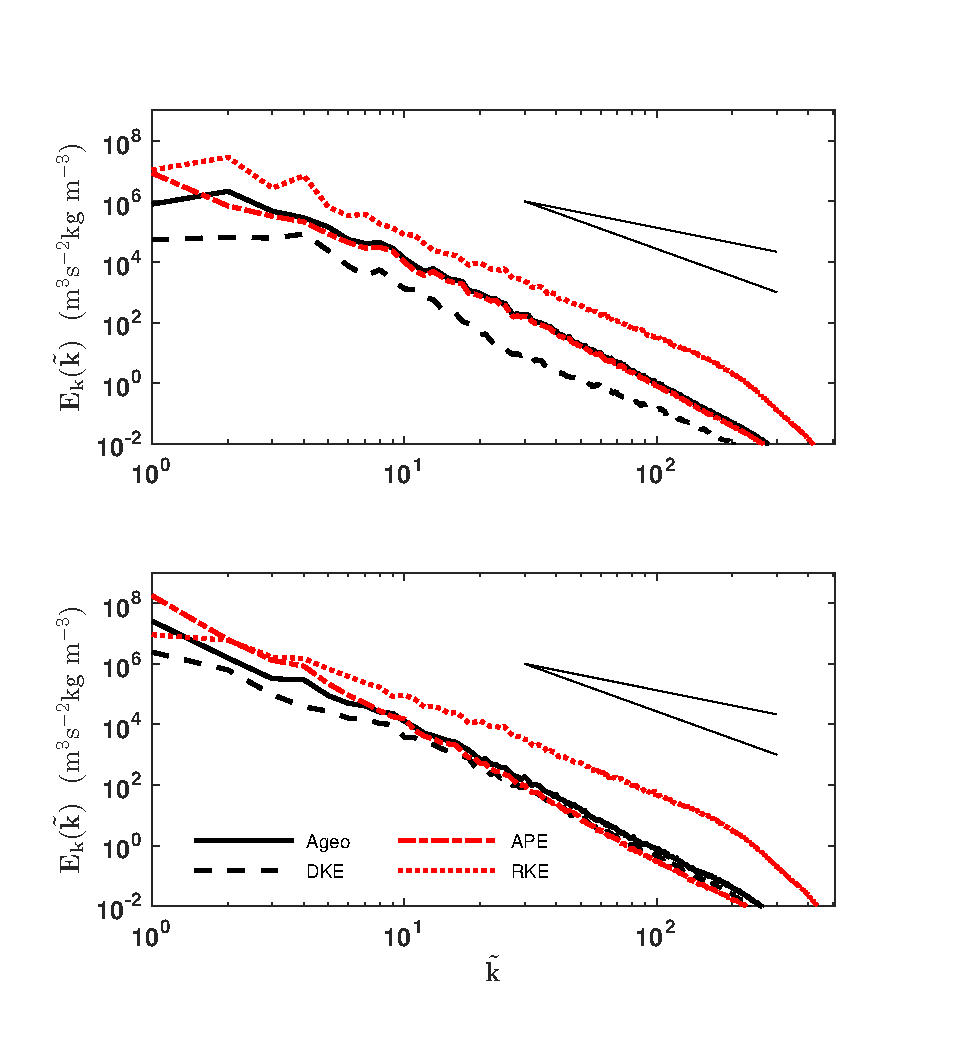
\includegraphics[scale=1]{Chapter4/img/Ageo_APEDKE_1-3}
\caption{Ageostrophic (black solid), DKE (black dashed), APE (red dash-dot), and RKE (red dotted) spectra for vertical modes 1 (top) and 3 (bottom). The wavenumber corresponding to $f/c_n$ is $\tilde{k} = 0.65$ for mode 1 and $\tilde{k} = 1.5$ for mode 3.}
\label{fig:Ageo_APEDKE_1-3}
\end{figure}

\begin{figure}[H]
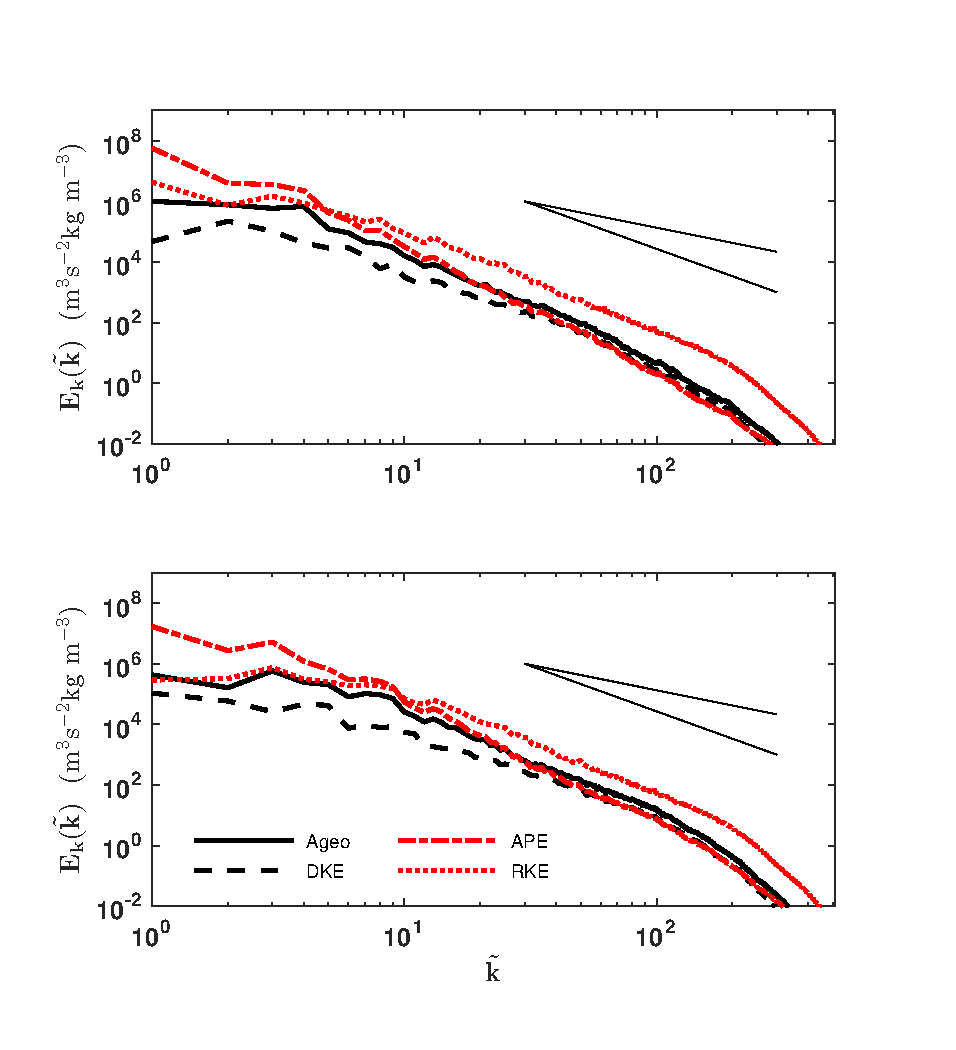
\includegraphics[scale=1]{Chapter4/img/Ageo_APEDKE_5-7}
\caption{The same as in Figure \ref{fig:Ageo_APEDKE_1-3}, but for vertical modes 5 (top) and 7 (bottom). The wavenumber corresponding to $f/c_n$ is  $\tilde{k} = 2.5$ for mode 5 and $\tilde{k} = 3.6$ for mode 7.}
\label{fig:Ageo_APEDKE_5-7}
\end{figure}

\begin{figure}[H]
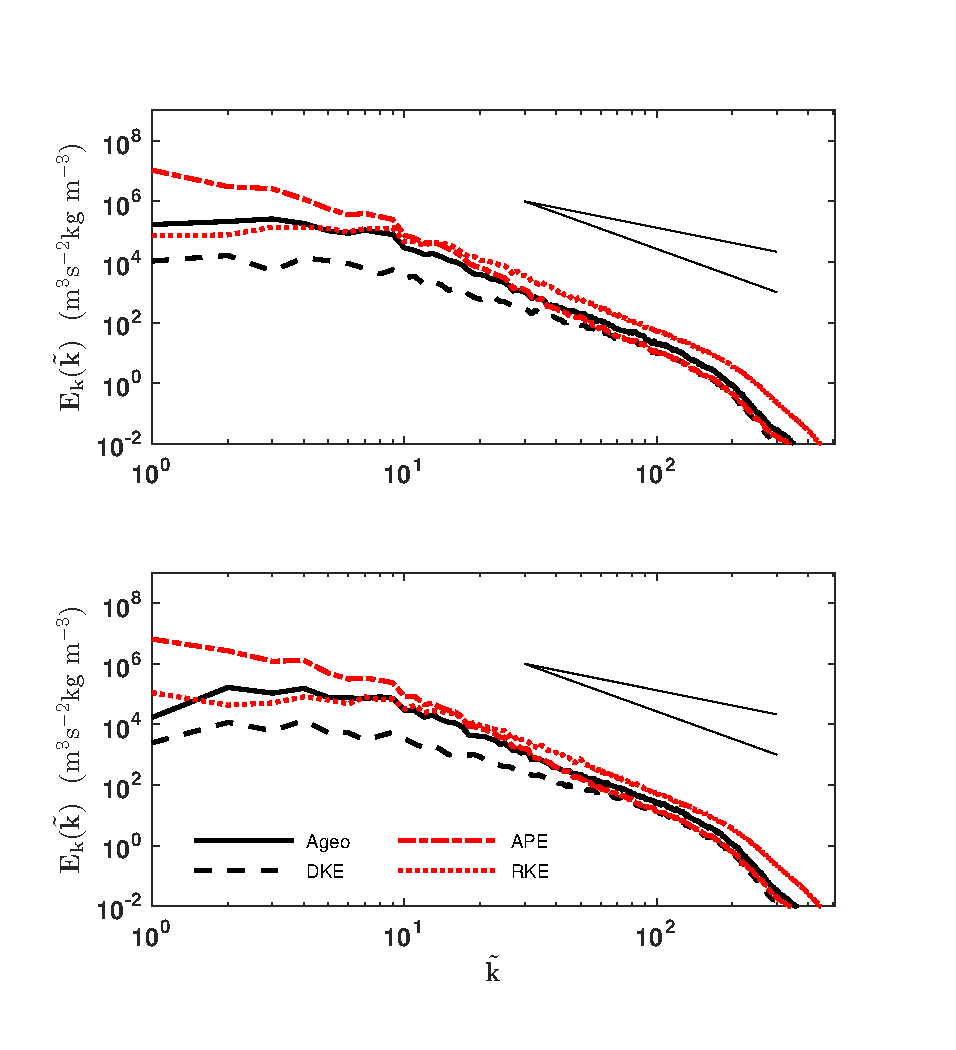
\includegraphics[scale=1]{Chapter4/img/Ageo_APEDKE_9-11}
\caption{The same as in Figure \ref{fig:Ageo_APEDKE_1-3}, but for vertical modes 9 (top) and 11 (bottom).  The wavenumber corresponding to $f/c_n$ is $\tilde{k} = 4.9$ for mode 9 and $\tilde{k} = 6.1$ for mode 11.}
\label{fig:Ageo_APEDKE_9-11}
\end{figure}

\begin{figure}[H]
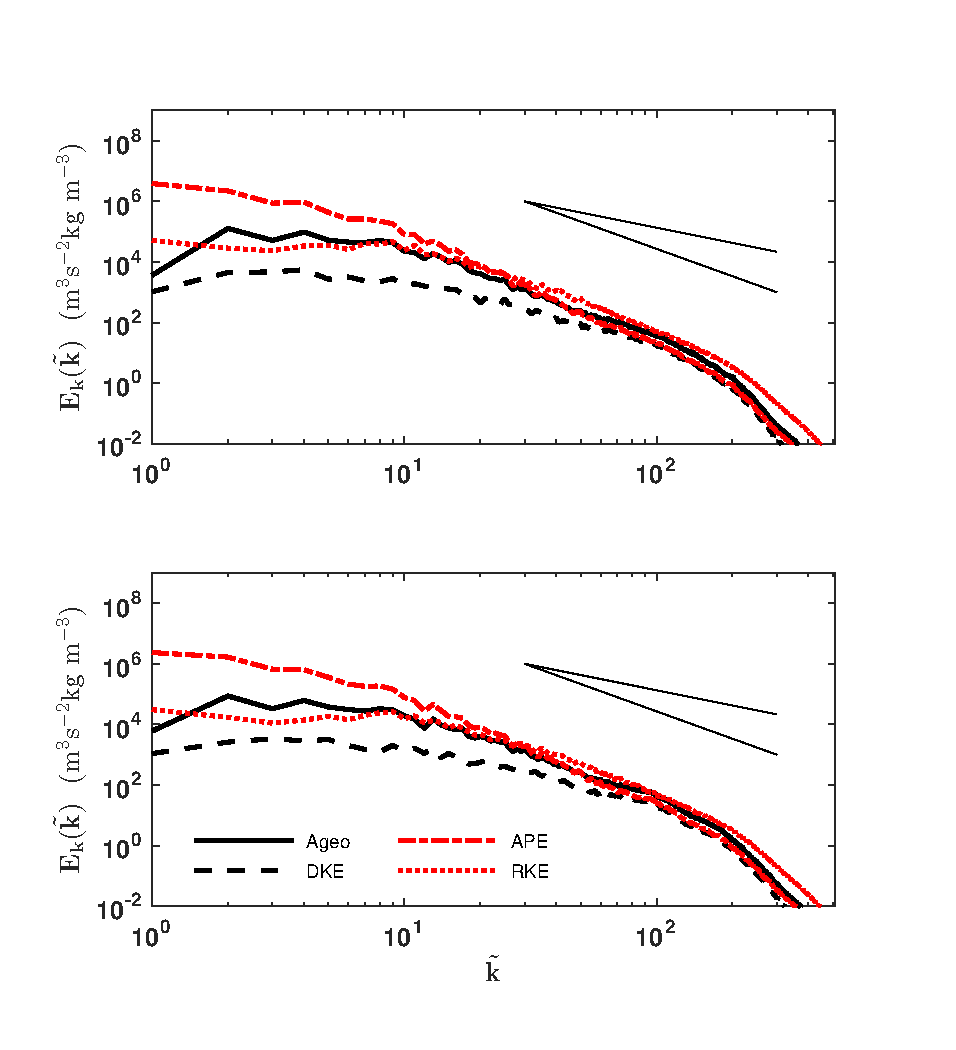
\includegraphics[scale=1]{Chapter4/img/Ageo_APEDKE_13-15}
\caption{The same as in Figure \ref{fig:Ageo_APEDKE_1-3}, but for vertical modes 13 (top) and 15 (bottom). The wavenumber corresponding to $f/c_n$ is $\tilde{k} = 7.5$ for mode 13 and $\tilde{k} = 8.9$ for mode 15.}
\label{fig:Ageo_APEDKE_13-15}
\end{figure}

\begin{figure}[H]
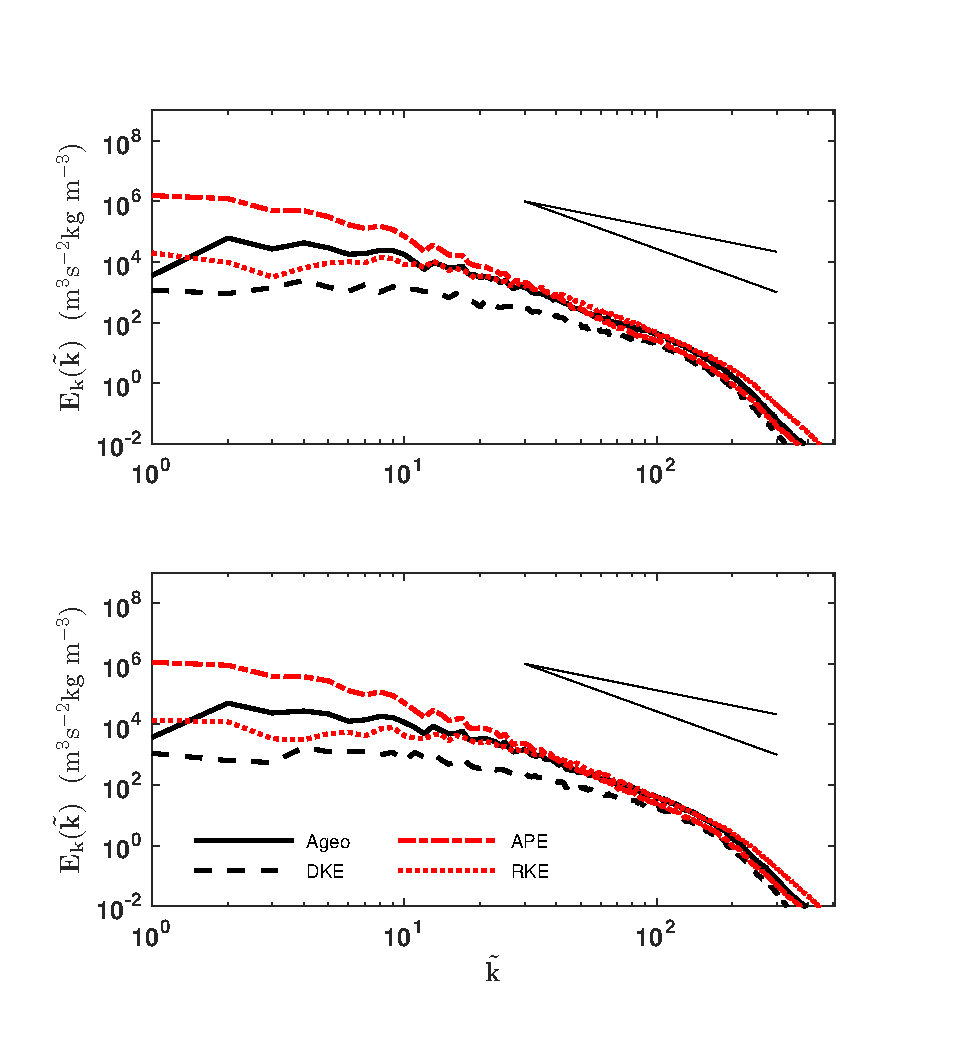
\includegraphics[scale=1]{Chapter4/img/Ageo_APEDKE_17-19}
\caption{The same as in Figure \ref{fig:Ageo_APEDKE_1-3}, but for vertical modes 17 (top) and 19 (bottom). The wavenumber corresponding to $f/c_n$ is $\tilde{k} = 10.3$ for mode 17 and $\tilde{k} = 11.8$ for mode 19.}
\label{fig:Ageo_APEDKE_17-19}
\end{figure}

\begin{figure}[H]
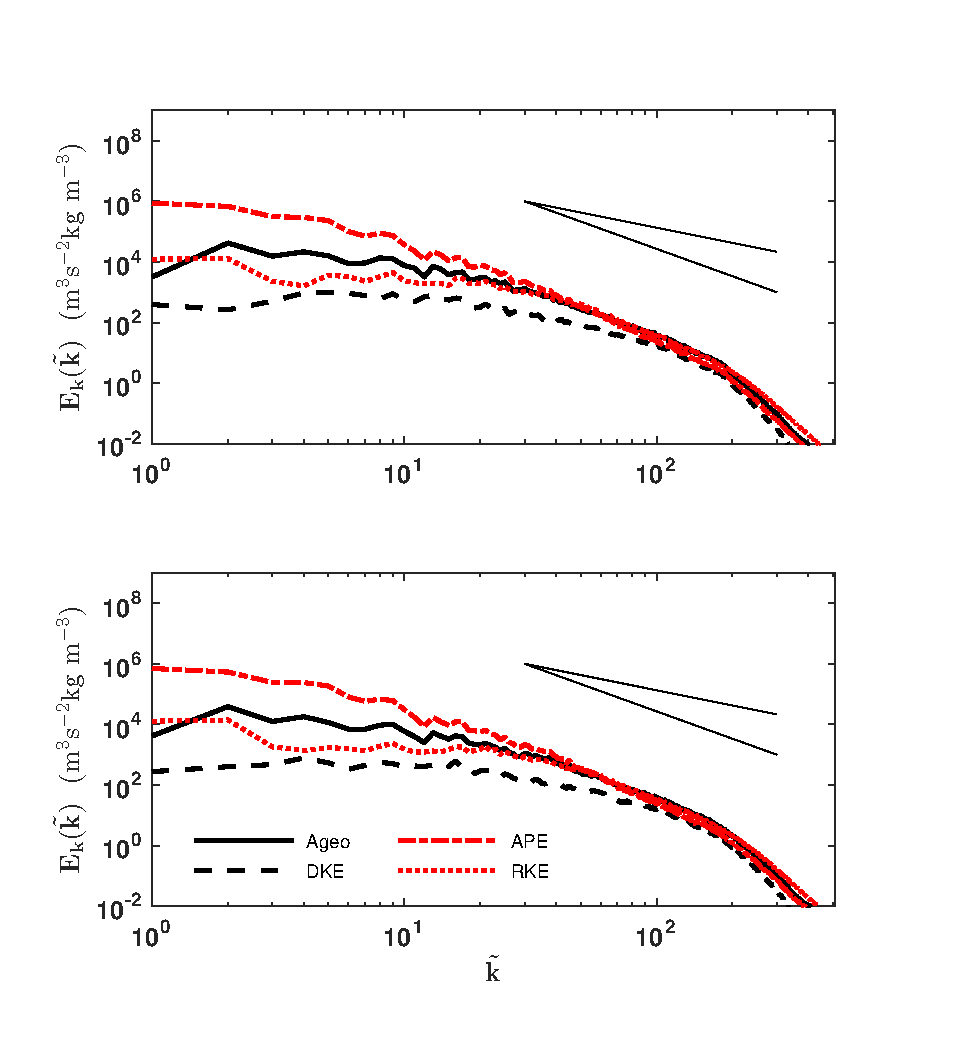
\includegraphics[scale=1]{Chapter4/img/Ageo_APEDKE_21-23}
\caption{The same as in Figure \ref{fig:Ageo_APEDKE_1-3}, but for vertical modes 21 (top) and 23 (bottom). The wavenumber corresponding to $f/c_n$ is $\tilde{k} = 13.4$ for mode 21 and $\tilde{k} = 15$ for mode 23.}
\label{fig:Ageo_APEDKE_21-23}
\end{figure}

\begin{figure}[H]
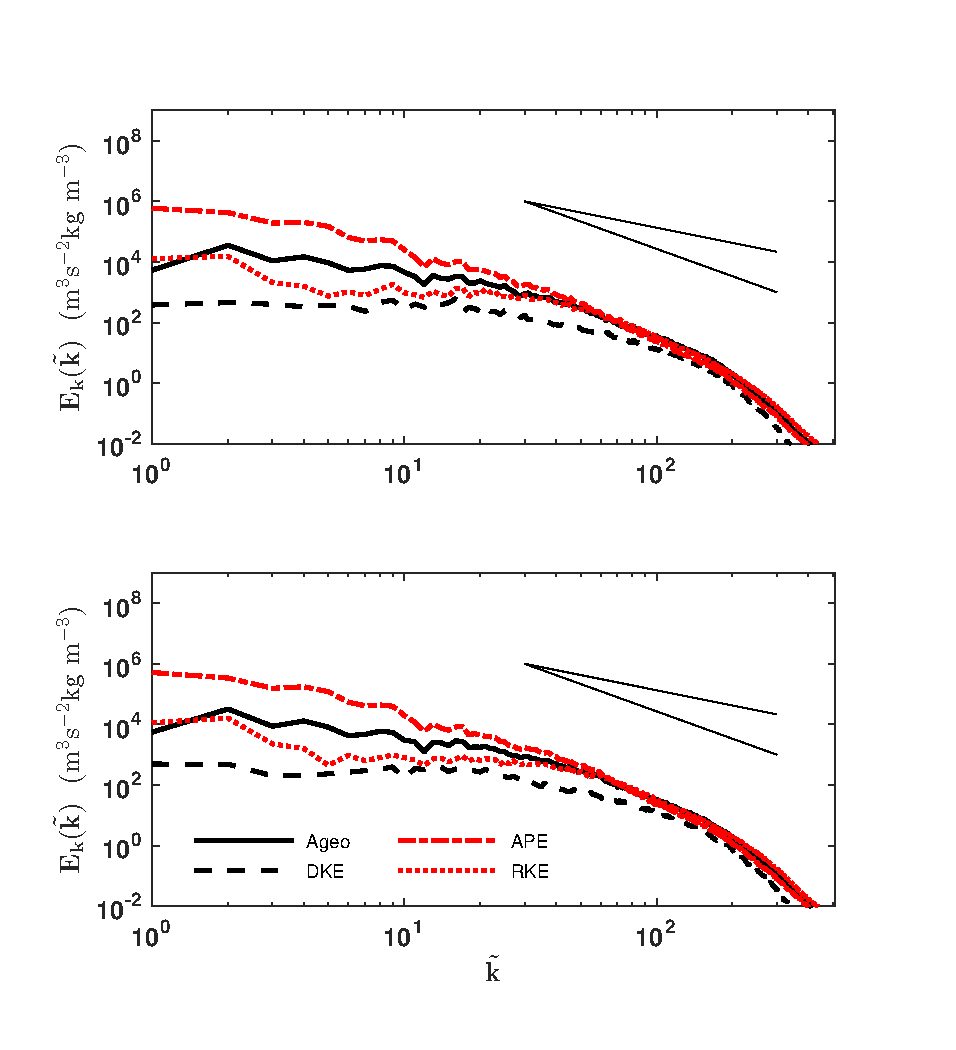
\includegraphics[scale=1]{Chapter4/img/Ageo_APEDKE_25-27}
\caption{The same as in Figure \ref{fig:Ageo_APEDKE_1-3}, but for vertical modes 25 (top) and 27 (bottom). The wavenumber corresponding to $f/c_n$ is $\tilde{k} = 16.6$ for mode 25 and $\tilde{k} = 18.3$ for mode 27.}
\label{fig:Ageo_APEDKE_25-27}
\end{figure}

\begin{figure}[H]
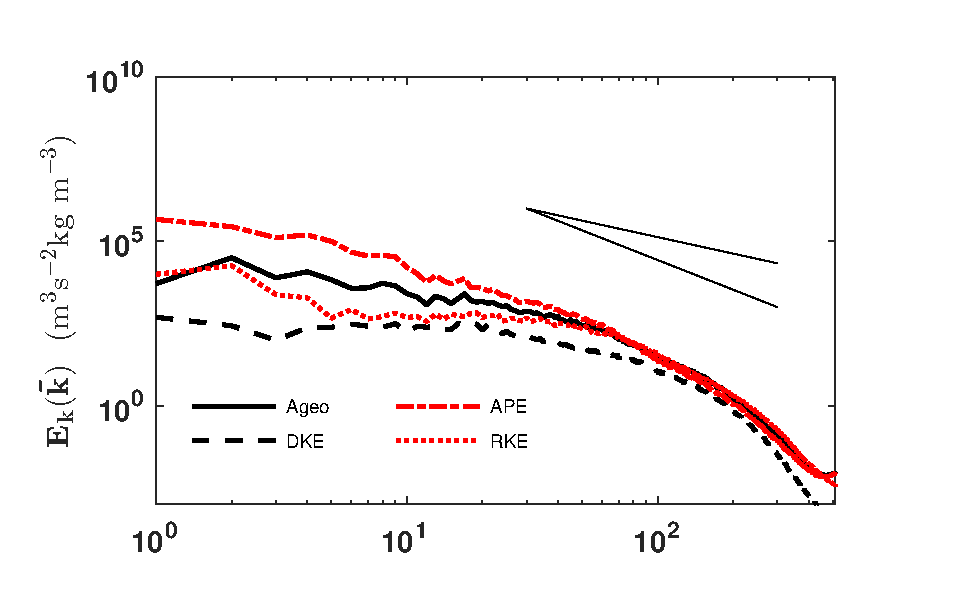
\includegraphics[scale=1]{Chapter4/img/Ageo_APEDKE_29}
\caption{The same as in Figure \ref{fig:Ageo_APEDKE_1-3}, but for vertical mode 29. The wavenumber corresponding to $f/c_n$ for this mode is $\tilde{k} = 20.1$.}
\label{fig:Ageo_APEDKE_29}
\end{figure}

In addition to examining the spectra of the individual vertical modes, it could be more enlightening to study the mesoscale slopes of the geostrophic, ageostrophic, and Helhmoltz modes as a function of vertical mode number. Table \ref{tab:slopes} shows the slope of the geostrophic, ageostrophic, RKE, and DKE in the mesoscale, calculated over the interval $6 \leq \tilde{k} \leq 60$. $R^2 > 0.94$ for every mode. Clearly, the general trend is that the slopes of all of the spectra decrease as the vertical mode number increases.  In addition to Table \ref{tab:slopes}, this can be more easily seen in the accompanying Figure \ref{fig:slopes}.\\

Overall, geostrophic mesoscale slopes are around -3 or steeper for vertical modes $<$ 15. The ageostrophic mesoscale spectrum shallows for vertical modes $>$ 10. The RKE and DKE spectra are much shallower than the geostrophic and ageostrophic spectra for largest values of $n$.

\begin{table}[H]
\begin{tabular}{c c c c c}
\hline
\textbf{Vertical Mode} & \textbf{Geostrophic Slope} & \textbf{RKE slope} & \textbf{Ageostrophic Slope} & \textbf{DKE slope}\\
\hline
Barotropic (0) & -3.6 & -3.6 & -4.0 & -3.1 \\
1 & -3.4 & -3.4 & -4.0 & -4.3\\
2 & -3.2 & -3.2 & -4.6 & -4.8\\
3 & -3.2 & -3.2 & -4.1 & -4.0\\
4 & -3.3 & -3.2 & -3.6 & -3.3\\
5 & -3.4 & -3.3 & -3.2 & -2.8\\
6 & -3.4 & -3.2 & -3.3 & -2.7\\
7 & -3.5 & -3.2 & -3.4 & -2.6 \\
8 & -3.5 & -3.1 & -3.4 & -2.5 \\
9 & -3.4 & -3.0 & -3.3 & -2.3 \\
10 & -3.4 & -2.8 & -3.2 & -2.2 \\
11 & -3.3 & -2.7 & -3.2 & -2.2 \\
12 & -3.2 & -2.6 & -3.0 & -2.1\\
13 & -3.2 & -2.4 & -2.9 & -2.0 \\
14 & -3.1 & -2.2 & -2.8 & -1.9\\
15 & -3.0 & -2.1 & -2.7 & -1.8\\
16 & -2.9 & -2.0 & -2.5 & -1.7\\
17 & -2.9 & -1.9 & -2.4 & -1.6\\
18 & -2.8 & -1.7 & -2.3 & -1.5\\
19 & -2.7 & -1.5 & -2.2 & -1.5\\
20 & -2.7 & -1.4 & -2.1 & -1.4\\
21 & -2.6 & -1.3 & -2.0 & -1.3\\
22 & -2.5 & -1.1 & -2.0 & -1.3\\
23 & -2.5 & -1.0 & -1.9 & -1.2\\
24 & -2.4 & -0.93 & -1.8 & -1.2\\
25 & -2.3 & -0.82 & -1.7 & -1.2\\
26 & -2.3 & -0.73 & -1.6 & -1.1\\
27 & -2.2 & -0.67 & -1.5 & -1.1\\
28 & -2.2 & -0.63 & -1.5 & -1.0\\
29 & -2.2 & -0.57 & -1.4 & -1.0 \\
30 & -2.1 & -0.56 & -1.4 & -0.96\\
\hline
\end{tabular}
\caption{The spectra slopes of the first 30 modes in the mesoscale.}
\label{tab:slopes}
\end{table}

\begin{figure}[H]
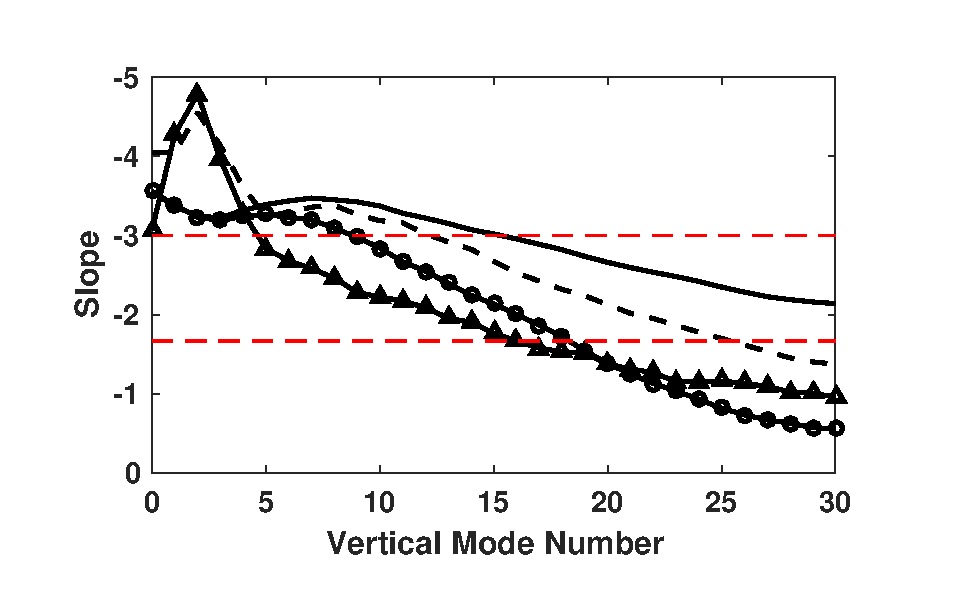
\includegraphics[scale=1]{Chapter4/img/slopes}
\caption{The mesoscale spectra slopes of the geostrophic (solid), ageostrophic (dashed), RKE (circles), and DKE (triangles) as a function of vertical mode number. Red dashed lines show references to $-3$ and $-5/3$ slopes. Note that the y-axis is reversed so that more negative values (i.e. steeper slope values) appear higher on the y-axis.}
\label{fig:slopes}
\end{figure}

Lastly, to determine the relative importance of each vertical mode in the full decomposition of the baroclinic jet into balanced vortical and inertia-gravity wave motion, the fraction of energy in each vertical mode is shown in Figure \ref{fig:modal_energy}. A large fraction of the energy is in the barotropic mode, so to help illustrate the contributions of the baroclinic modes, Figure \ref{fig:modal_energy_nobaro} shows the energy distribution, excluding the barotropic mode.\\

Since the mesoscale spectra are of particular interest, we also calculate the fraction of energy of each vertical mode contained in the mesoscale. This mesoscale energy is decomposed into geostrophic and ageostrophic components and displayed in Figure \ref{fig:meso_GeoAgeo}. The KE and APE in each vertical mode in shown as well in Figure \ref{fig:meso_KEPE}.

\begin{figure}[H]
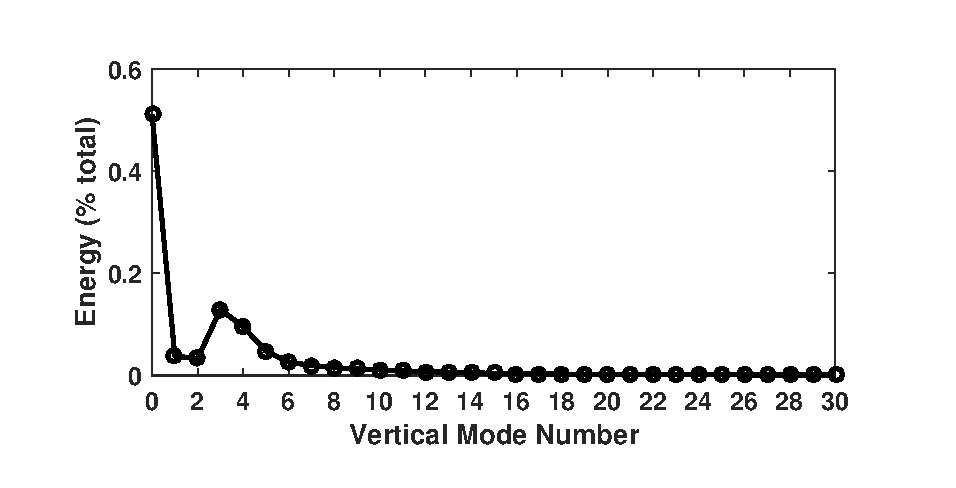
\includegraphics[scale=1]{Chapter4/img/modal_energy}
\caption{The fraction of energy in each vertical mode.}
\label{fig:modal_energy}
\end{figure}
\vspace{-0.2in}
\begin{figure}[H]
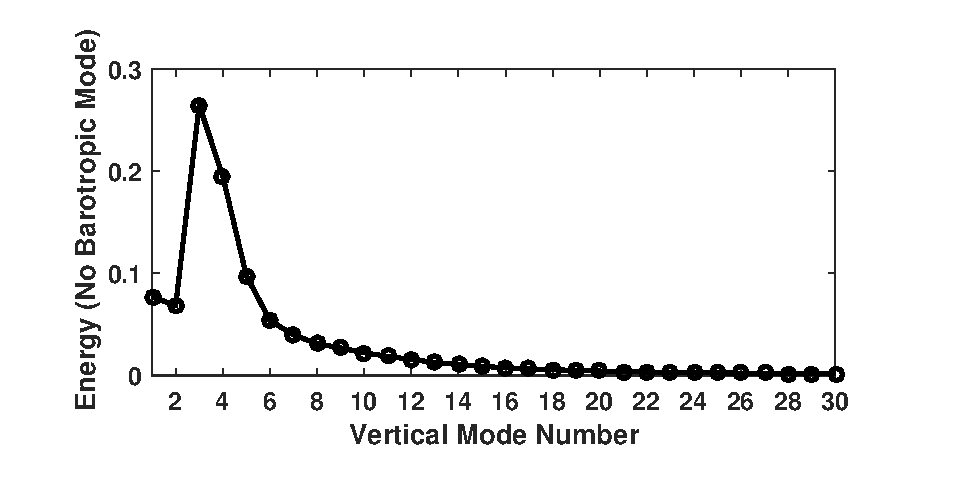
\includegraphics[scale=1]{Chapter4/img/modal_energy_nobaro}
\caption{As in Figure \ref{fig:meso_GeoAgeo},  excluding the barotropic mode.}
\label{fig:modal_energy_nobaro}
\end{figure}

\begin{figure}[H]
\vspace{0cm}
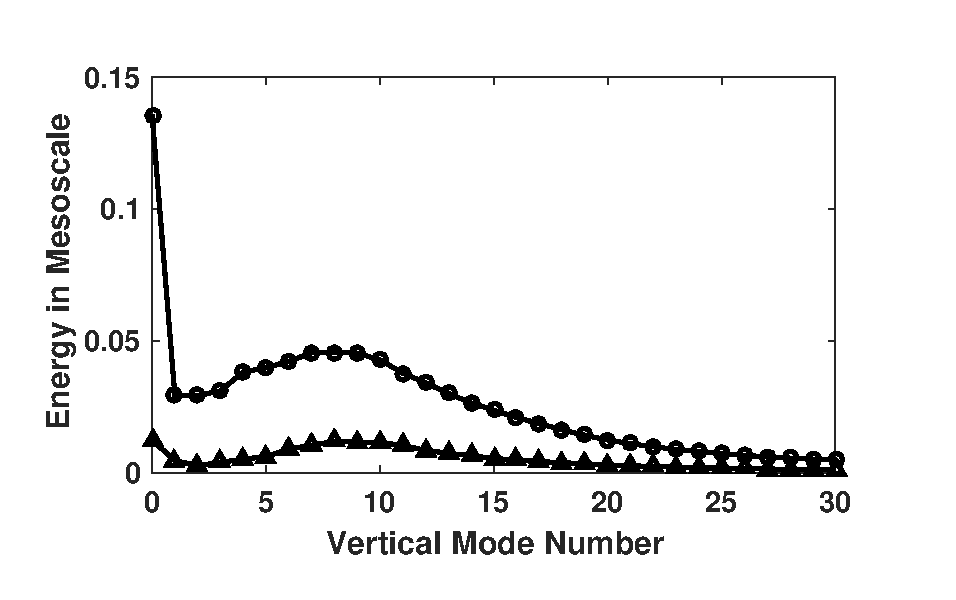
\includegraphics[scale=1]{Chapter4/img/meso_GeoAgeo}
\vspace{0cm}
\caption{The fraction of mesoscale energy in each vertical mode for the geostrophic (circles) and ageostrophic (triangles) modes.}
\label{fig:meso_GeoAgeo}
\end{figure}

\begin{figure}[H]
\vspace{0cm}
\includegraphics[scale=1]{Chapter4/img/meso_KEPE}
\vspace{0cm}
\caption{As in Figure \ref{fig:meso_GeoAgeo}, but for the KE (circles) and APE (triangles).}
\label{fig:meso_KEPE}
\end{figure}

\subsection{Combining the Vertical Modes}
Due to the orthogonality of the normal mode decomposition, by summing the first 30 vertical modes the normal mode decomposition can be compared to the depth-averaged Helmholtz decomposition of the full velocity fields (see Figure \ref{fig:totalGeoAgeo}).  As seen, the geostrophic and RKE slopes are -3.1 and -2.7, respectively. There is a bit more discrepancy between the ageostrophic and DKE slopes with values of -2.7 and -1.9, respectively. 

\begin{figure}[H]
\includegraphics[scale=1]{Chapter4/img/totalGeoAgeo}
\vspace{-0.5in}
\caption{The first 30 vertical modes summed together (geostrophic, black solid; ageostrophic, black dashed) compared to the vertically-averaged RKE (red dash-dot) and DKE (red dotted). $-3$ and $-5/3$ references are shown in the upper right.}
\label{fig:totalGeoAgeo}
\end{figure}

From  Figure \ref{fig:meso_GeoAgeo}, it appears that (excluding the barotropic mode), a lot of the mesoscale energy lies between vertical modes 5 and 15. To investigate this,  Figure \ref{fig:meso_RKEDKE} shows the normal mode decomposition and Helmholtz decomposition summed over vertical modes 5 through 15. The geostrophic and ageostrophic slopes are -3.3 and -3.1, while the RKE and DKE slopes are -2.9 and -2.3.\\

\begin{figure}[H]
\includegraphics[scale=1]{Chapter4/img/meso_RKEDKE}
\caption{The geostrophic (black solid) and ageostrophic (black dashed) compared to the RKE (red dash-dot) and DKE (red dotted) spectra summed over vertical modes 5 through 15. $-3$ and $-5/3$ references are shown in the upper right.}
\label{fig:meso_RKEDKE}
\end{figure}

In Chapter \ref{ch:ch5}, we discuss these results and offer an explanation for the mesoscale spectra of the full decomposition as seen in Figure \ref{fig:totalGeoAgeo}.
\chapter{Discussion and Conclusions}
\label{ch:ch5}

\section{Discussion}
In this section, we first analyze the overall decomposition, i.e\ the results of the first 30 vertical modes summed together compared to the full-depth averaged Helmholtz decomposition. Next, we discuss the energy spectra in each of the vertical modes. Finally, some concluding remarks are given.

\subsection{Overall Analysis}
One of the first noticeable features from the geostrophic and ageostrophic decompositions in Figure \ref{fig:totalGeoAgeo} is the relatively steep slope associated with the ageostrophic mesoscale spectrum. Compared to the $-3$ and $-5/3$ slopes of the rotational and divergent kinetic energy in the literature, the summation of the first 30 vertical modes resulted in mesoscale spectra slopes of $-3.1$ and $-2.7$ for the geostrophic and ageostrophic modes, respectively. Though the geostrophic and RKE mesoscale spectra slopes are somewhat in agreement, at -3.1 and -2.7, respectively, the mesoscale slope of the ageostrophic spectrum at $-2.7$ is much steeper than the DKE spectrum at $-1.9$.\\

Before we discuss the discrepancies between the geostrophic/ageostrophic decomposition and the RKE/DKE decomposition, we turn our attention to the shallower RKE spectrum and the steeper DKE spectrum when compared to the $-3$ and $-5/3$ mesoscale slopes found in the literature. Since the baroclinic instability simulation was computed on a grid with evenly-spaced pressure levels, this translates to a clustering of points near the surface that get increasingly spaced apart higher in the atmosphere in $z$ coordinates. The strong surface fronts therefore have more impact on the energy spectrum of the instabilities, which cause shallowing in the large scales of the vortical motion. Previous research by Peng et al.\ has indeed shown shallower spectra near the ground \cite{Peng2013}. Additionally, the large Rossby number can also be causing a reduction in the large scales of vortical motion, instead transferring some of that energy to the ageostrophic component at the mesoscale (e.g.\ \cite{Bartello2010}).\\

The ageostrophic spectrum contains more total energy over the entire synoptic scale and mesoscale when compared to the DKE. This is due to the available potential energy (APE) in the ageostrophic mode. Since the baroclinic instabilities grow by converting APE to kinetic energy, at large scales we expect a large amount of potential energy as well as kinetic energy to drive the downward cascade of energy. At large scales and throughout the mesoscale, we see that the potential energy is decreasing with increasing wavenumber. At dimensionless wavenumbers of  $\tilde{k} > 200$, which corresponds to wavelengths smaller than approximately $25$ km, the ageostrophic and DKE spectra are well aligned. At these small scales, much of the APE has been converted to kinetic energy just before the numerical dissipation removes energy from the system. The RKE spectrum is similar to the geostrophic spectrum, suggesting that most of the vortical energy is in fact kinetic. At the smallest horizontal scales, the total kinetic energy in the domain (i.e.\ the RKE and DKE) appears to contain more energy than the total energy (i.e.\ geostrophic and ageostrophic modes combined), which would be unphysical. This can be explained from the exclusion of vertical modes higher than 30. Since increasing vertical mode number corresponds to decreasing equivalent depth, the energy contribution at higher vertical modes is increasingly concentrated in larger horizontal wavenumbers. We expect that by including more vertical modes, it would be seen that the total energy at large wavenumbers would be greater than or equal to the kinetic energy. We now examine the energy spectra at each vertical mode number and discuss how decreasing equivalent depths associated with increasing mode numbers affect the mesoscale slopes.\\

\subsection{Modal Analysis}
The energy spectra of the vertical modes exhibit a changing behavior in both the geostrophic and ageostrophic decomposition, as the mode number increases.  We separate discussion into the barotropic and baroclinic modes.\\

\subsubsection{Barotropic Mode}
The barotropic mode spectra has steep slopes in the geostrophic and RKE spectra, at $-3.6$ in the mesoscale for both. The ageostrophic slope is even steeper, at a value of $-4.0$ in the mesoscale. \\

The most interesting feature of the barotropic mode occurs in the DKE spectrum, where the  mesoscale slope is much shallower at $-2.5$ as seen in Figure \ref{fig:barotropicKEPE}. This stark contrast between the ageostrophic and DKE spectra occurs only in the barotropic mode. An interesting feature to note is that the DKE spectrum also contains significantly less energy than the ageostrophic mode, meaning that potential energy is the main contributor to the ageostrophic energy. Indeed, for all but the largest horizontal length scales, the geostrophic and potential energy spectra are in agreement in Figure \ref{fig:barotropicKEPE}, implying that the geostrophic mode has very little APE.

\subsubsection{Baroclinic Modes}
\label{sec:baroclinicanalysis}
We now turn our attention to the remaining vertical modes, the baroclinic modes. Before discussing the mathematical properties of the geostrophic, ageostrophic, and Helmholtz spectra, qualitative properties of the baroclinic modes are examined.\\

We first look at the geostrophic and rotational spectra for the baroclinic modes. For the first several baroclinic modes, the geostrophic mode and RKE spectra align except for the largest horizontal scales. As the vertical mode number increases, the RKE energy at larger horizontal scales begins to separate from the geostrophic energy. By vertical mode 11, the geostrophic spectrum contains more energy compared to RKE spectrum at the larger end of the mesoscale ($6 \leq \tilde{k} < 10$), while they are approximately equal for the smaller end of the mesoscale ($\tilde{k} > 15$). By around vertical mode 25, the geostrophic spectrum contains more energy than the RKE throughout the entire mesoscale, only aligning for horizontal scales corresponding to $<100$ km wavelengths.\\

For the first 10 baroclinic modes, the mesoscale slope of the geostrophic spectrum stays roughly constant, fluctuating around $-3.5$, while the rotational spectrum slope decreases slightly from around $-3.5$ to $-3$ over this same range. From vertical modes 5 through 15, where the mesoscale energy peaks (see Figure \ref{fig:meso_GeoAgeo}), the geostrophic spectrum is steeper than $-3$ throughout, while the RKE mesoscale slope decreases below $-3$ beginning at mode 10. Beyond mode 10, the RKE mesoscale spectrum begins to shallow at a faster rate than the geostrophic spectrum, indicating that potential energy is energizing the mesoscale.\\

The ageostrophic and DKE spectra have slightly different behavior occurring throughout the vertical modes. In the first several vertical modes, the ageostrophic spectrum has more energy than the DKE at all horizontal scales due to the inclusion of potential energy. Vertical mode 2 is especially interesting because of the large increase in DKE mesoscale slope seen in Figure \ref{fig:slopes}.  As the vertical modes increase, the energy in the larger horizontal scales decreases and the mesoscale slopes shallow, similar to the rotational and RKE spectra. However, a difference between the geostrophic/RKE spectra and the ageostrophic/DKE spectra is that the energy in the mesoscale actually increases with increasing vertical mode number for the first 10 vertical modes which contributes to the mesoscale shallowing (see Figure \ref{fig:meso_GeoAgeo}). Beyond mode 10, the energy in the mesoscale of the ageostrophic and DKE spectra starts to decrease again as in the geostrophic and RKE spectra.\\

The ageostrophic and DKE mesoscale spectra both have a sharp spike at vertical mode 2. Excluding the barotropic mode, this also contains the most synoptic scale energy of any vertical mode, as well as relatively small mesoscale energy in comparison. The difference between the very energetic large scale and less energetic mesoscale in vertical mode 2 can help explain the sharp spike at vertical mode 2 for the ageostrophic and DKE in Figure \ref{fig:slopes}, when also taking into account the kinetic and potential energy in the mesoscale shown in Figure \ref{fig:meso_KEPE}. From mode 5 onward, the ageostrophic spectrum continues to be steeper than the DKE spectrum, but it also shallows at a faster rate when compared to the DKE spectrum. Past vertical mode 20, the DKE spectrum becomes steeper than the RKE spectrum.\\

We now provide a mathematical justification for the spectra of the normal mode and Helmholtz decompositions shown in Figures \ref{fig:GeoAgeo_RKEDKE_1-3} - \ref{fig:GeoAgeo_RKEDKE_29}. Equation (\ref{eq:amplitudes}) can be written in terms of the Helmholtz decomposition for a specific $\mathbf{k}$ and $n$ to give

\begin{align}
A^0_{\mathbf{k},n} &= \frac{1}{\sqrt{c^2_n K^2 + f^2}} \left[ c_n (ik\widehat{V} - il\widehat{U}) + f \widehat{\eta} \right],\\
&= \frac{c_n}{\sqrt{c^2_n K^2 + f^2}}\widehat{\zeta} + \frac{f}{\sqrt{c^2_n K^2 + f^2}} \widehat{\eta},\\
&= \frac{\widehat{\zeta}}{\sqrt{K^2 + (f/c_n)^2}} + \frac{(f/c_n) \widehat{\eta}}{\sqrt{K^2 + (f/c_n)^2}}.
\end{align}

The resulting amplitude for the geostrophic mode can then be written 

\begin{align}
|A^0_{\mathbf{k},n}|^2 &= \frac{1}{K^2 + (f/c_n)^2} \left[ \left(\widehat{\zeta}^* + \frac{f}{c_n} \widehat{\eta}^*\right) \left(\widehat{\zeta} + \frac{f}{c_n} \widehat{\eta}\right)\right],\\
&= \frac{1}{K^2 + (f/c_n)^2} \left[ |\widehat{\zeta}|^2 + \left(\frac{f}{c_n}\right)^2 |\widehat{\eta}|^2 + \frac{f}{c_n} \left(\widehat{\eta}^*\widehat{\zeta} + \widehat{\eta}\widehat{\zeta}^*\right)\right]\label{eq:geoBreakdown}.
\end{align}
The ratio $c_n/f$ is essentially the Rossby deformation radius, and so it can be helpful to analyze the geostrophic and ageostrophic spectra at length scales much larger or smaller than the deformation radius. For $ K \gg f/c_n$, as is the case for the first several vertical modes at most values of $K$, then 
\begin{align}
|A^0_{\mathbf{k},n}|^2 \approx \frac{|\widehat{\zeta}|^2}{K^2},
\end{align}
which means that the geostrophic spectrum is approximately equal to the RKE. As the ratio $f/(Kc_n)$ increases, the geostrophic energy has additional contributions from the two right-most quantities in equation (\ref{eq:geoBreakdown}). This is why for the first several vertical modes, the geostrophic and RKE spectra are approximately equal over all horizontal length scales. Indeed, by referring to Figures \ref{fig:Geo_APERKE_1-3} - \ref{fig:Geo_APERKE_29}, the geostrophic mode transitions from being made up of almost entirely RKE in vertical mode 1 (see \ref{fig:Geo_APERKE_1-3}), to being made up of mostly APE for $\tilde{k} < 20$ and mostly RKE for $\tilde{k} > 20$ in vertical mode 11 (see Figure \ref{fig:Geo_APERKE_9-11}). By vertical mode 25 (see Figure \ref{fig:Geo_APERKE_25-27}), the geostrophic mode over the entire mesoscale is mostly from the APE.  As the vertical mode increases, and thus $c_n$ decreases, $K$ must increase for the RKE and geostrophic spectra to align again. This shows that for decreasing equivalent depths, the vortical motion is taking place at smaller horizontal length scales. By vertical mode 29, the geostrophic and RKE spectra do not coincide until $\tilde{k} \approx 100$, meaning much of the vortical motion is taking place at the sub-mesoscale.\\

We can also write the ageostrophic mode in terms of the Helmholtz decomposition, resulting in

\begin{align}
|A^+_{\mathbf{k},n}|^2 & = \frac{1}{2K^2 \alpha^2} \left[\left( -f \widehat{\zeta}^* - i\alpha \widehat{\delta}^* + c_n K^2 \widehat{\eta}^* \right)\left( -f \widehat{\zeta} + i\alpha\widehat{\delta} + c_n K^2 \widehat{\eta}\right)\right]\\
&= \frac{1}{2K^2\alpha^2} \left ( \left[f^2 |\widehat{\zeta}|^2 + \alpha^2 |\widehat{\delta}|^2 + c^2_n K^4 |\widehat{\eta}|^2\right] + if\alpha \widehat{\zeta}^* \widehat{\delta} + i \alpha c_n K^2 \widehat{\delta}^* \widehat{\eta} - f c_n K^2 \widehat{\zeta}^* \widehat{\eta} + \hbox{c.c.} \right),
\end{align}
where $\alpha^2 = c^2_nK^2 + f^2$ is used for notational simplicity and $\hbox{c.c.}$ means complex conjugate. This can be written in terms of the ratio $f/c_n$ 
\begin{align}
\begin{split}
|A^+_{\mathbf{k},n}|^2  &= \frac{1}{2K^2} \frac{ (f/c_n)^2}{K^2 + (f/c_n)^2} |\widehat{\zeta}|^2 + \frac{1}{2K^2} |\widehat{\delta}|^2 + \frac{1}{2\left(1 + \left(\frac{f}{c_nK}\right)^2\right)} |\widehat{\eta}|^2\\
&~+ \frac{i(f/c_n)}{2K^2 \sqrt{K^2  + (f/c_n)^2}} \widehat{\zeta}^* \widehat{\delta} + \frac{i}{2\sqrt{K^2 + (f/c_n)^2}} \widehat{\delta}^* \widehat{\eta} - \frac{f/c_n}{2\left(K^2 + (f/c_n)^2 \right)} \widehat{\zeta}^* \widehat{\eta} + \hbox{c.c.}, \label{eq:ageoPlusBreakdown}
\end{split}
\end{align}
For the other ageostrophic mode, $A^-_{\mathbf{k},n}$, the result is very similar:
\begin{align}
\begin{split}
|A^-_{\mathbf{k},n}|^2  &= \frac{1}{2K^2} \frac{ (f/c_n)^2}{K^2 + (f/c_n)^2} |\widehat{\zeta}|^2 + \frac{1}{2K^2} |\widehat{\delta}|^2 + \frac{1}{2\left(1 + \left(\frac{f}{c_nK}\right)^2\right)} |\widehat{\eta}|^2\\
&~- \frac{i(f/c_n)}{2K^2 \sqrt{K^2  + (f/c_n)^2}} \widehat{\zeta}^* \widehat{\delta} - \frac{i}{2\sqrt{K^2 + (f/c_n)^2}} \widehat{\delta}^* \widehat{\eta} - \frac{f/c_n}{2\left(K^2 + (f/c_n)^2 \right)} \widehat{\zeta}^* \widehat{\eta} + \hbox{c.c.}, \label{eq:ageoMinusBreakdown}
\end{split}
\end{align}
such that 
\begin{align}
|A^0_{\mathbf{k},n}|^2 + |A^-_{\mathbf{k},n}|^2 + |A^-_{\mathbf{k},n}|^2 = |\widehat{U}|^2 + |\widehat{V}|^2 + |\widehat{\eta}|^2.
\end{align}

 For $K \gg f/c_n$,  the ageostrophic spectrum can be approximated by
\begin{align}
|A^+_{\mathbf{k},n}|^2 \approx \frac{1}{2K^2} |\widehat{\delta}|^2 + \frac{1}{2} |\widehat{\eta}|^2 + \frac{i}{2K} \widehat{\delta}^* \widehat{\eta} + \hbox{c.c.}, \label{eq:ageoLargeScales}
\end{align}
 interpreted as being made up from the DKE and the available potential energy, with cross-terms between the two also appearing. As the vertical modes increase and $c_n$ decreases, the contribution to the ageostrophic mode from the APE decreases.\\

 In vertical mode 1 (see Figure \ref{fig:Ageo_APEDKE_1-3}), the ageostrophic spectrum is made up almost entirely of APE at all but the largest horizontal length scales. Equation (\ref{eq:ageoLargeScales}) shows that the DKE contribution is independent of the ratio $f/Kc_n$. Therefore, the full DKE energy is contained in the ageostrophic mode, but the DKE contains about an order of magnitude less than the APE throughout the mesoscale. The RKE contribution for vertical mode 1 is negligible for the mesoscale, since $K \gg f/c_n$. \\
 
In vertical mode 11 (see Figure \ref{fig:Ageo_APEDKE_9-11}), the APE spectrum contains more energy than the ageostrophic spectrum for $\mathbf{\tilde{k}} < 30$. In this regime, the ratio $f/Kc_n$ is no longer negligible, and the APE contribution to the ageostrophic mode decreases, while the RKE contribution to the ageostrophic mode increases. By $\mathbf{\tilde{k}} > 40$, the ageostrophic spectrum crosses the APE spectrum. Here $f/Kc_n$ is becoming smaller and the ageostrophic spectrum is once again well approximated by equation (\ref{eq:ageoLargeScales}).\\
 
 In vertical mode 25, the APE and ageostrophic spectra do not cross until around $\mathbf{\tilde{k}} \approx 60$, meaning that the DKE contribution to the ageostrophic spectrum is important in determining the mesoscale slope, despite that the DKE spectrum contains several orders of magnitude less energy than the APE spectrum.\\
 
Figure \ref{fig:totalGeoAgeo} becomes easier to understand when combining all of the above along with Figures  \ref{fig:modal_energy} and \ref{fig:modal_energy_nobaro}, where it can be seen that a majority of the total energy is contained in the first 6 vertical modes. \\

For the first 5 modes, where the equivalent depth is relatively large, the geostrophic spectrum is composed of mostly RKE in the mesoscale. Beginning at mode 6, the geostrophic spectrum is a blend of the RKE and APE in the large end of the mesoscale ($6 < \tilde{k} < 10$), while the small end of the mesoscale ($10 < \tilde{k} < 60$) remains dominated by RKE. This trend continues for increasing vertical modes, with the APE becoming increasingly important at small wavenumbers, while at the same time the APE influence expands to higher horizontal wavenumbers. By mode 15, the mesoscale is strongly determined by the APE and the RKE only dominates at microscales.\\

The make up of the ageostrophic portion of motion is a more intricate combination of the APE, DKE, and RKE. In the barotropic mode, where $f/Kc_n$ is negligible throughout the mesoscale, the ageostrophic spectrum is dominated by APE since the DKE is orders of magnitude smaller. For the first 5 vertical modes, RKE plays an increasingly important role in the large horizontal scales, while the APE contribution decreases from the increasing $f/Kc_n$ ratio. Modes 4 and 5 have a shallower slope in the mesoscale when compared to the APE, due to the increased importance of the shallower spectra of the DKE and RKE. By mode 11, the APE spectrum contains more energy than the ageostrophic spectrum throughout the entire mesoscale. \\

The APE contribution at each vertical mode for both the geostrophic and ageostrophic spectra explains the mesoscale slopes in Figure \ref{fig:totalGeoAgeo}. The geostrophic spectrum is for the most part similar to the RKE spectrum, but slightly steeper due to the increasing APE contribution to the mesoscale spectrum as the vertical modes increase. The steepness of the ageostrophic mesoscale spectrum when compared to the DKE spectrum can be explained by the importance of the APE in the first few vertical modes. As the DKE and RKE become more significant in the ageostrophic energy around vertical mode 5, the ageostrophic spectrum shallows.
\newpage
\section{Conclusions}
The shallowing of the energy spectrum at the mesoscale has been well-observed in atmospheric turbulence and plays an important role in the energy budget, connecting large scales containing vast amounts of energy to the microscales where dissipation occurs. Understanding the underlying processes of the mesoscale shallowing can help provide insight into the turbulent cascade of energy in the mesoscale.\\

The Helmholtz decomposition is commonly used on the horizontal velocity fields to separate a rotating, stratified fluid into vortical and gravity wave motion. The resulting solenoidal and irrotational fields are then crudely used as a proxy for the vortical motion and gravity waves. The Helmholtz decomposition, while simple, does not include the effects of potential energy in the two dominant modes. Furthermore, the balanced vortical mode has small, but non-zero, divergence, which is not present in the solenoidal component of the Helmholtz decomposition. Similarly, rotational energy in inertia-gravity waves is omitted by the irrotational component, as the name suggests. \\

In our work, we presented an improved decomposition over the Helmholtz decomposition. By first decomposing the vertical structure of the baroclinic jet into into normal modes, we obtain geostrophic and ageostrophic modes that offer a more physically realistic decomposition of the flow compared to the Helmholtz decomposition. However, our normal mode decomposition is still an approximation to the true dynamics taking place in the atmosphere. For example, the set of equations used in the derivation of the vertical structure make use of the hydrostatic approximation, which is not valid across all scales. A normal mode decomposition that considers a non-hydrostatic set of equations would of course be more accurate, but the hydrostatic approximation greatly simplifies the underlying mathematics and the simulation studied in this thesis remains fairly hydrostatic. Though the geostrophic mode in our approach is still divergence-free like the Helmholtz decomposition, the ageostrophic mode contains rotational kinetic energy as well as potential energy which affects the shape of the energy spectrum.\\

Furthermore, the normal mode decomposition allows an extension of the discussion to explicitly include not only horizontal length scales, like the Helmholtz decomposition, but also vertical scales as a result of the eigenvalues in the vertical structure equation. These eigenvalues turn out to be important in determining the overall shape of the geostrophic and ageostrophic spectra.\\

In terms of the energy contained in the vertical modes, the most energy was contained in the first 6 vertical modes. However, most of this energy is in the synoptic scale. If we restrict our attention to the mesoscale, the most energetic modes actually range from around vertical mode 5 to vertical mode 15. For these modes, the equivalent depths from the eigenvalue problem are small enough that the ratio $f/Kc_n = \mathcal{O}(1)$ at the mesoscale. In this regime, complicated contributions from the APE,  DKE, and RKE make up the geostrophic and ageostrophic modes.\\
 
By summing over all of the vertical normal modes, the geostrophic and ageostrophic spectra can be compared to the Helmholtz decomposition. In general, we find the mesoscale slope of the geostrophic spectrum to be steeper than the RKE spectrum, with values of $-3.1$ and $-2.7$, respectively. In the vertical mode numbers where the mesoscale energy is the highest, the increased importance of the APE on the geostrophic mode causes the spectrum to steepen, shifting it away from the RKE spectrum.\\

The difference between the normal mode decomposition and the Helmholtz decomposition is most visible when examining the ageostrophic and DKE spectra. While the RKE and geostrophic mode contain similar amounts of energy over the entire spectrum, the ageostrophic mode contains almost an order of magnitude more energy than the DKE at every wavenumber up until the sub-mesoscale. The mesoscale slopes of the ageostrophic and DKE spectra also have a much starker contrast compared to the geostrophic and RKE spectra, with mesoscale slopes of $-2.7$ for the ageostrophic mode and $-1.9$ for the DKE. The inclusion of APE and, to a lesser extent, RKE is the main source of the difference between the DKE and ageostrophic mesoscale slopes. The ageostrophic mode is comprised of mainly DKE and APE when the ratio $f/Kc_n$ is small, with the APE contribution becoming less important and RKE becoming more important as $f/Kc_n$ increases. In the vertical modes where mesoscale energy is the highest, the transition of the ageostrophic spectrum from being mostly influenced by APE to being mostly influenced by DKE and RKE takes place around the middle of the mesoscale. This transition leads to the mesoscale shallowing seen in the ageostrophic mode, but the APE prevents it from completely agreeing with the DKE.\\


%=====================================================================

%\chapter*{APPENDICES}
%\addcontentsline{toc}{chapter}{APPENDICES}
%%======================================================================
%\chapter[PDF Plots From Matlab]{Matlab Code for Making a PDF Plot}
%\label{AppendixA}
%% Tip 4: Example of how to get a shorter chapter title for the Table of Contents 
%%======================================================================
%\section{Using the GUI}
%Properties of Matab plots can be adjusted from the plot window via a graphical interface. Under the Desktop menu in the Figure window, select the Property Editor. You may also want to check the Plot Browser and Figure Palette for more tools. To adjust properties of the axes, look under the Edit menu and select Axes Properties.
%
%To set the figure size and to save as PDF or other file formats, click the Export Setup button in the figure Property Editor.
%
%\section{From the Command Line} 
%All figure properties can also be manipulated from the command line. Here's an example: 
%\begin{verbatim}
%x=[0:0.1:pi];
%hold on % Plot multiple traces on one figure
%plot(x,sin(x))
%plot(x,cos(x),'--r')
%plot(x,tan(x),'.-g')
%title('Some Trig Functions Over 0 to \pi') % Note LaTeX markup!
%legend('{\it sin}(x)','{\it cos}(x)','{\it tan}(x)')
%hold off
%set(gca,'Ylim',[-3 3]) % Adjust Y limits of "current axes"
%set(gcf,'Units','inches') % Set figure size units of "current figure"
%set(gcf,'Position',[0,0,6,4]) % Set figure width (6 in.) and height (4 in.)
%cd n:\thesis\plots % Select where to save
%print -dpdf plot.pdf % Save as PDF
%\end{verbatim}

%----------------------------------------------------------------------
% END MATERIAL
%----------------------------------------------------------------------

% B I B L I O G R A P H Y
% -----------------------

% The following statement selects the style to use for references.  It controls the sort order of the entries in the bibliography and also the formatting for the in-text labels.
\bibliographystyle{plain}
% This specifies the location of the file containing the bibliographic information.  
% It assumes you're using BibTeX (if not, why not?).
\cleardoublepage % This is needed if the book class is used, to place the anchor in the correct page,
                 % because the bibliography will start on its own page.
                 % Use \clearpage instead if the document class uses the "oneside" argument
\phantomsection  % With hyperref package, enables hyperlinking from the table of contents to bibliography             
% The following statement causes the title "References" to be used for the bibliography section:
\renewcommand*{\bibname}{References}

% Add the References to the Table of Contents
\addcontentsline{toc}{chapter}{\textbf{References}}

\bibliography{References/library.bib}
% Tip 5: You can create multiple .bib files to organize your references. 
% Just list them all in the \bibliogaphy command, separated by commas (no spaces).

% The following statement causes the specified references to be added to the bibliography% even if they were not 
% cited in the text. The asterisk is a wildcard that causes all entries in the bibliographic database to be included (optional).
%\nocite{*}

\end{document}
